% Paquetes.
\documentclass[10pt,twoside,a4paper]{book}
\usepackage[utf8]{inputenc}
\usepackage[spanish]{babel}
\usepackage{graphicx}
\usepackage{subfigure}
\usepackage[hidelinks]{hyperref}
\usepackage[hmarginratio=1:1]{geometry}
\usepackage{multirow}
\usepackage{float}
\usepackage[eurosym,right]{eurofont}
\usepackage{listings}
\usepackage[strict]{chngpage}
\usepackage{array}
\usepackage{color, colortbl}
\usepackage{longtable}
\usepackage{caption}

\definecolor{Gray}{gray}{0.9}
\lstset{basicstyle=\ttfamily\scriptsize}

% Comienza el documento.
\begin{document}
\pagestyle{empty}

\begin{center}
{\bf\large UNIVERSIDADE DE SANTIAGO DE COMPOSTELA}

\vspace{0.5cm}
{\bf\large ESCOLA TÉCNICA SUPERIOR DE ENXEÑARÍA}

\vspace{1.5cm}

\includegraphics[width=5cm]{figuras/logo_usc.jpg}

\vspace{2cm}
{\bf\Large Plataforma Web para la Validación de Experimentación en Aprendizaje Automático y Minería de Datos}

\vspace{1cm}
{\normalsize TRABAJO DE FIN DE GRADO}
\end{center}

\begin{flushright}
\vspace{6cm}
{\bf Realizado por:} \\
Adrián Canosa Mouzo \\
~ \\
{\bf Dirigido por:} \\
Ismael Rodríguez Fernández \\
Alberto J. Bugarín Díz \\
Manuel Mucientes Molina \\
\end{flushright}


\cleardoublepage
\chapter*{Agradecimientos}

\thispagestyle{empty}

\textit{El presente Trabajo Fin de Grado se ha desarrollado en el marco del proyecto de I+D+i ``QTEMP: Descripción lingüística de fenómenos complejos: cuantificadores borrosos generalizados en proposiciones temporales (TIN2011-29827-C02-02)", coordinado entre el Grupo de Sistemas Intelixentes de la USC y el European Centre for Soft Computing, y financiado por el Ministerio de Economía y Competitividad en el período 2012-2014.}
\cleardoublepage

% Numeración y cabeceras.
\pagenumbering{roman}
\setcounter{page}{1}
\pagestyle{plain}
\tableofcontents
\listoffigures

% Ahora se incluyen los capítulos. Se cambia la numeración y las cabeceras.
\cleardoublepage
\pagenumbering{arabic}
\setcounter{page}{1}
\pagestyle{headings}
\setlength{\parskip}{3mm}
%***************************************************************************************************************************

\chapter{Introducción}
En el contexto tecnológico actual, en donde el Big Data es un recurso cada vez más utilizado, el rol
del analista de datos (data scientist) se está convirtiendo en una profesión emergente y de elevada
demanda. Un analista de datos es aquel profesional que reúne, analiza e interpreta los datos obtenidos
con el objetivo de sacar ciertas conclusiones de ellos y así tomar diferentes decisiones, con las que
aumentar la productividad en una organización. Relacionado con el analista de datos, un nuevo rol emergente
en muchas empresas es el de CDO (\textit{``Chief Data Officer"}). Este rol es el responsable de la gestión
y la utilización de la información como un activo para toda la empresa. El analista de datos combina diferentes
habilidades, especialmente las técnicas de la minería de datos y del aprendizaje automático (DM\&ML).

Según Mitchell \cite{mitchell}, una definición de aprendizaje automático sería la siguiente: un programa
de ordenador aprende a partir de una experiencia E a realizar una tarea T (de acuerdo con una medida de
rendimiento P), si su rendimiento al realizar T, medido con P, mejora gracias a la experiencia E. La
minería de datos, por otra parte, es un campo de las ciencias de la computación referido al proceso que trata
de descubrir patrones en grandes volúmenes de conjuntos de datos \cite{mineria}. Para ello utiliza, entre
otros métodos, técnicas estadísticas para deducir estos patrones y tendencias que existen en los datos. Por
lo general, estos patrones no pueden ser detectados mediante exploración tradicional debido a la complejidad o
la gran cantidad de datos.

Una de las tareas más importantes que se deben llevar a cabo en el aprendizaje automático es la
validación de resultados obtenidos por los algoritmos de aprendizaje. El método estándar más aceptado
en la actualidad es el de la aplicación de test estadísticos sobre los experimentos, que, entre otras
utilidades, apoyan la toma de decisiones, como por ejemplo la elección del algoritmo más adecuado.

En este proyecto hemos creado y desarrollado una plataforma para asistir al analista de
datos en el proceso de validación de resultados. Para ello, se extendió una librería de test
estadísticos, se crearon servicios web para facilitar su consulta y se desarrolló una interfaz web
que hace uso de estos servicios. El objetivo es que el analista pueda introducir en la web los datos obtenidos
mediante experimentación y seleccionar el test estadístico que desee utilizar para que, de forma automática, la
plataforma muestre los resultados de la aplicación del test. Así, la plataforma permitirá de un modo fácil y
centralizado la validación de resultados mediante el uso de test estadísticos.

La herramienta se incorporará en la lista de aplicaciones disponibles a través de la web del
CiTIUS para su acceso. El impacto y difusión del resultado del proyecto tiene el potencial de ser amplio,
ya que en la actualidad no existe ninguna herramienta que centralice la aplicación de los test estadísticos de
mayor utilidad para la validación de algoritmos de aprendizaje automático y que, además, resulte fácil de usar.

%***************************************************************************************************************************

\section{Objetivos del proyecto}
El proyecto se centra en crear y desarrollar una plataforma web para asistir al analista de datos
en el proceso de validación de los resultados obtenidos de diferentes algoritmos de aprendizaje. Para ello,
habrá que realizar las siguientes tareas:
\begin{enumerate}
\item Completar y extender una librería de test estadísticos, actualmente implementada en el lenguaje Python.

La librería estará formada por test paramétricos, test para evaluar las condiciones de aplicación de los test
paramétricos (para la normalidad y homocedasticidad), así como test no paramétricos. Estos test se verán en
detalle a lo largo del capítulo \ref{contraste} en las secciones \ref{parametricos}, \ref{condiciones} y
\ref{no_parametricos} respectivamente. La librería a extender se denomina ``nonparametric.py", y los test de
normalidad y homocedasticidad, así como la prueba  $\mathcal{T}$ de Student se tomarán de la librería de estadística
de Python SciPy (scipy.stats). El listado de test para el proyecto es el siguientes:

- Normalidad: Shapiro-Wilk, D’Agostino–Pearson y Kolmogorov–Smirnov.

- Homocedasticidad: Levene.

- Paramétricos: t-test, ANOVA, Bonferroni.

- No paramétricos: Wilcoxon, Friedman, Iman-Davenport, Rangos Alineados de Friedman, Quade, Bonferroni-Dunn,
Holm, Finner, Hochberg, Li, Shaffer.

\item Crear los servicios web en Python, basados en REST, que hagan disponible el acceso a los
test estadísticos vía web.

Los servicios REST están basados en los métodos HTTP (POST y GET para este proyecto). Asimismo, las peticiones
a los servicios web de los test incluirán todos los datos necesarios (petición completa e independiente) para
que el servidor no tenga que mantener ningún estado para procesar la petición. Los datos a transmitir (datos del
analista, resultados obtenidos por los test) con REST se podrán transferir mediante XML, JavaScript Object
Notation (JSON), o ambos. Cada servicio dispondrá de varias URIs distintas en función de los parámetros para dar
mayor versatilidad a la API.

\item Desarrollar una interfaz web (HTML + JavaScript) para facilitar el uso de los test sobre los
datos introducidos por el analista de datos.

Las tecnologías que se emplearán para desarrollarla serán: HTML, JavaScript y CSS. Un requisito para el proyecto
es que el analista pueda aplicar los test de la forma más sencilla posible, por lo que se tendrá en cuenta este
aspecto en el desarrollo.
\end{enumerate}

%***************************************************************************************************************************

\section{Organización del documento}
La finalidad de este documento es la de presentar los desarrollos realizados para resolver correctamente los objetivos definidos, explicando para ello cada una de las partes que componen la plataforma web y las tareas realizadas a lo largo del proceso.
\begin{itemize}
\item En el \textit{\textbf{capítulo 2}} se explican los conceptos básicos manejados en el proyecto. Para ello, se realiza un análisis detallado del contraste de hipótesis, tratando los conceptos básicos con ejemplos. Además, se explica la finalidad y funcionamiento de cada uno de los test disponibles en la plataforma.
\item El \textit{\textbf{capítulo 3}} hace un análisis de los requisitos identificados en el proyecto, utilizando para ello las historias de usuario empleadas en la metodología del proyecto.
\item El \textit{\textbf{capítulo 4}} describe la gestión del proyecto. Incluye el análisis de riesgos, la metodología de desarrollo, la gestión de la configuración, la planificación temporal y el análisis de costes.
\item En el \textit{\textbf{capítulo 5}} se propone una arquitectura a alto nivel del sistema y se definen cada una
de las partes de las que constará, así como las herramientas de diseño y desarrollo utilizadas.
\item El \textit{\textbf{capítulo 6}} explica tanto el diseño como la implementación a bajo nivel de la arquitectura
propuesta.
\item El \textit{\textbf{capítulo 7}} se definen las pruebas establecidas para poder comprobar que la herramienta es válida y que los objetivos se han cumplido. Se detallan además los resultados de las mismas.
\item Por último, en el \textit{\textbf{capítulo 8}} se establecen aquellas conclusiones derivadas de la realización del
proyecto, además de una breve indicación de lo que podría ser mejorable o ampliable en un futuro.
\end{itemize}

%***************************************************************************************************************************
\cleardoublepage
%***************************************************************************************************************************

\chapter{Contraste de hipótesis} \label{contraste}
El contraste de hipótesis, también conocido como test estadísticos, se engloba en el ámbito de la
Inferencia Estadística, que es la parte de la estadística que estudia cómo sacar conclusiones generales
(sujetas a un determinado grado de fiabilidad o significancia) para toda la población a partir del
estudio de una muestra. En nuestro caso, se tratará de sacar conclusiones de los resultados obtenidos por
diferentes algoritmos sobre distintos conjuntos de datos para determinar, por ejemplo, si los algoritmos
tienen un rendimiento significativamente diferente y por lo tanto no se pueden considerar iguales.

El \textbf{contraste de hipótesis} es uno de los problemas más comunes dentro de la inferencia
estadística. En él se contrasta una hipótesis estadística. Por ejemplo:\\\\
\textit{Un ingeniero de software afirma que la media de los resultados obtenidos por un algoritmo
de aprendizaje automático es 10. ¿Se podría desmentir la afirmación del ingeniero?}\\\\
El planteamiento del contraste sería el siguiente  ($\mu$ indica media poblacional):
\begin{center}
$ \mu = 10 $

$ \mu \neq 10 $
\end{center}

Para tomar una decisión (desmentir o no la afirmación), hay que basarse en los datos de una muestra, para
comprobar si en efecto la media de los resultados es 10 (media muestral). Para ello, se podría establecer una
regla de decisión sobre la cual se basaría nuestra decisión final. Por ejemplo: si la media obtenida está
próxima a la indicada por el ingeniero (10), entonces se podría afirmar que dice la verdad. Si por el
contrario la muestra nos proporciona una media muy distinta a 10, entonces se puede concluir que la evidencia
desmiente la afirmación del ingeniero sobre el algoritmo en cuestión. Esto plantea cuándo  se puede considerar
que la media es lo suficientemente distinta como para determinar que la afirmación del ingeniero es errónea. Por
ejemplo si la media de la muestra es 8.5, ¿se podría desmentir la afirmación inicial? El contraste de hipótesis
nos proporciona una forma de establecer este criterio y poder rechazar o aceptar la afirmación inicial.

%***************************************************************************************************************************

\section{Hipótesis nula y alternativa}
En todo contraste de hipótesis siempre se dan dos posibilidades o hipótesis, las cuales se representan con
los siguientes símbolos:
\begin{center}
$H_0:$ hipótesis nula

$H_1:$ hipótesis alternativa
\end{center}
\begin{itemize}
\item $H_0$: es la hipótesis que se supone cierta de partida, es decir, es la hipótesis que establece que lo que
indica la muestra es solamente debido a la variación aleatoria entre la muestra y la población.
\item $H_1$: es la hipótesis alternativa y es la que reemplazará a la hipótesis nula si ésta es rechazada. $H_1$
establece que lo que indica la muestra es verdadero, y representa a toda la población.
\end{itemize}
A modo de ejemplo, supongamos que unos programadores están trabajando en la optimización de un algoritmo
de aprendizaje. El objetivo es mejorar el algoritmo de forma que los resultados que proporcione sean menores
de 100. Se toma una muestra de los resultados obtenidos por el nuevo algoritmo optimizado y se observa que la
media de la muestra es de 92. Si no hubiera incertidumbre en la media muestral, entonces se podría concluir
que la modificación reduciría los resultados a 92. Sin embargo, siempre existe incertidumbre en la media
muestral. La media poblacional en realidad será poco mayor o menor a 92.

Los programadores están preocupados de que el nuevo algoritmo en realidad no mejore al anterior, es decir, que
la media poblacional pudiera ser mayor o igual a 100. Quieren saber si esta preocupación está justificada. Se ha
observado una muestra con media de 92 y existen dos posibles interpretaciones, o como se ha mencionado más arriba,
dos tipos de hipótesis que serán contrastadas más adelante mediante un determinado test estadístico:
\begin{enumerate}
\item La media poblacional es mayor o igual a 100 (la media muestral es, por tanto, menor debido sólo a la
variación aleatoria de la media poblacional). El nuevo algoritmo no mejorará al anterior.
\item La media poblacional es menor que 100, y la media muestral lo refleja. El nuevo algoritmo sí mejorará
al anterior.
\end{enumerate}
La primera interpretación sería la hipótesis nula o $H_0$. La segunda, la hipótesis alternativa o $H_1$, como se
comentó más arriba.

En este caso, los programadores están preocupados de que la hipótesis nula sea cierta. Un test estadístico o
prueba de hipótesis hallará una medida cuantitativa de la factibilidad de la hipótesis nula (denominado
estadístico de contraste, que para este ejemplo viene dado por la media obtenida en la muestra) y se podrá
decir a los programadores (después de que el test tome la decisión) si su preocupación está o no justificada.
Por tanto, a modo de resumen este ejemplo nos proporciona dos hipótesis:
$$H_0: \mu \geq 100 \mbox{ vs. } H_1: \mu < 100$$

La realización de un contraste de hipótesis no consiste en decidir cuál de las dos hipótesis ($H_0$, $H_1$) es más
creíble, sino en decidir si la muestra proporciona o no suficiente evidencia para descartar $H_0$. Para realizar la
prueba de hipótesis o test estadístico se pone la hipótesis nula en juicio, es decir se empieza suponiendo que $H_0$
es verdadera. Se podría poner como analogía el supuesto de \textit{``En un juicio, el acusado siempre es inocente
hasta que se demuestre lo contrario."} Esto es:
\begin{center}
$H_0:$ el acusado es inocente

$H_1:$ el acusado es culpable
\end{center}
y, mientras no se tenga suficiente evidencia para aceptar $H_1$, hay que creer que lo que dice $H_0$ es cierto. La
muestra aleatoria proporcionará la evidencia. Si el juicio (test o prueba de hipótesis) determina que el acusado
es inocente, sólo se puede decir que no se tiene suficiente evidencia para asegurar que el acusado es culpable,
mientras que si aceptamos la hipótesis alternativa, se estará bastante seguro de que el acusado sí es culpable.

%***************************************************************************************************************************

\section{Estadístico de contraste} \label{estadistico}
Los test estadísticos o pruebas de hipótesis, calculan internamente una medida cuantitativa que proporciona la
factibilidad de la hipótesis nula. Esta medición se extrae de la muestra proporcionada. Por ejemplo, si queremos
contrastar la hipótesis de que la media poblacional es 5, un estadístico a calcular puede ser la media de una
muestra. En este caso, la muestra viene determinada por los resultados obtenidos por los algoritmos y cada uno de
los test tiene una forma particular de hallar este estadístico mediante una fórmula que lo caracteriza. Estos
estadísticos siguen una determinada distribución de probabilidad. Por ejemplo, en este proyecto los test
implementados harán uso de estadísticos que siguen distribuciones como:
\begin{itemize}
\item Distribución normal $\mathcal{N}$ (p. ej. test de Wilcoxon).
\item Distribución chi-cuadrado $\chi^2$ (p. ej. test de Friedman).
\item Distribución $\mathcal{F}$ de Fisher-Snedecor (p. ej. test de Iman-Davenport).
\item Distribución $\mathcal{T}$ de Student (p. ej. t-test).
\end{itemize}
La figura \ref{fig:pdf}, nos muestra el aspecto que presentan las distintas distribuciones de probabilidad. Las
distribuciones dependen de ciertos parámetros para determinar su forma ($\mu$, $\sigma^2$...): 
\begin{figure}[h]
\centering
\subfigure[Distribución $\mathcal{N}$ con media $\mu$ y varianza $\sigma^2$.]{
\label{fig:pdfa}
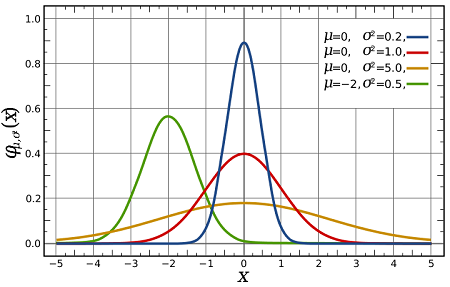
\includegraphics[width=5cm,height=3cm]{figuras/pdf_normal.png} }
\subfigure[Distribución $\chi^2$ con $K$ grados de libertad.]{
\label{fig:pdfb}
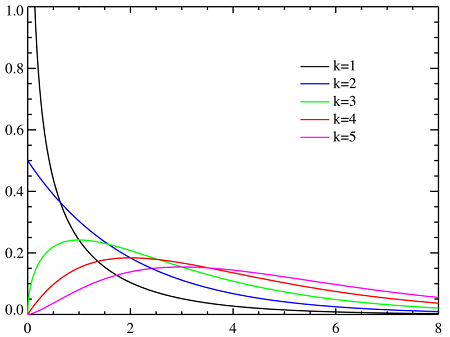
\includegraphics[width=5cm,height=3cm]{figuras/pdf_chi_cuadrado.png} }
\end{figure}
\begin{figure}[h]
\centering
\subfigure[Distribución $\mathcal{F}$ con $d1$ y $d2$ grados de libertad.]{
\label{fig:pdfc}
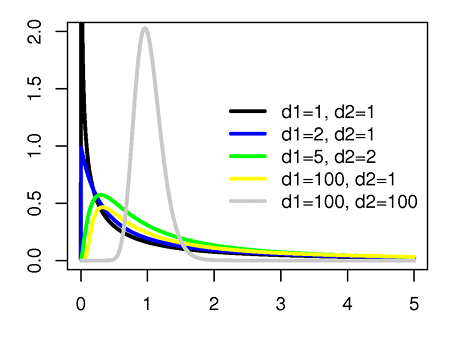
\includegraphics[width=5cm,height=3cm]{figuras/pdf_f.png} }
\subfigure[Distribución $\mathcal{T}$ con $K$ grados de libertad.]{
\label{fig:pdfd}
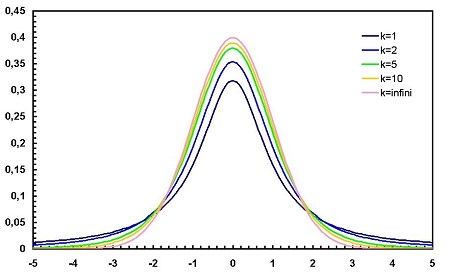
\includegraphics[width=5cm,height=3cm]{figuras/pdf_t_student.jpg} }
\caption{Distribuciones de probabilidad.}
\label{fig:pdf}
\end{figure}
\newline
Como podemos ver en la figura \ref{fig:pdf}, la distribución normal presenta $\mu$ y $\sigma^2$ como parámetros.
Éstos indican media y varianza respectivamente. La varianza, es una medida de dispersión que indica cómo se
distribuye la población. Por ejemplo: en una distribución normal de media 0 y varianza 1 (línea roja en la figura \ref{fig:pdfa}), aproximadamente el $68\%$ de la población se encuentra en el intervalo $[-1,1]$,
ya que el área bajo la curva es de 0.68. Por tanto, la probabilidad de que un individuo de la población se
encuentre en ese intervalo es del 68\%. Si un estadístico sigue una distribución normal con media $\mu$ y
varianza $\sigma^2$, se expresa como:
\[ \mbox{Estadístico} \sim N(\mu,\sigma^2) \]
En las distribuciones $\chi^2$ y $\mathcal{T}$ de Student se habla del parámetro $K$ o grados de libertad ($d1$ y $d2$  en
la distribución $\mathcal{F}$ de Fisher-Snedecor). La media y la varianza de estas tres distribuciones vendrán
determinadas por el parámetro $K$. Cuando se habla de grados de libertad se está haciendo referencia al número de valores
que se pueden elegir libremente en una muestra. Por ejemplo: una muestra con dos datos y media 5 si el primer dato
toma el valor 4 entonces necesariamente el segundo dato debe de ser 6 (para lograr la media de 5). En este caso,
se tienen:
\begin{center}
$N - 1$ grados de libertad, donde $N$ es el tamaño de la muestra.
\end{center}
Se hallan con la fórmula $N-R$, donde $N$ es el número de individuos en la muestra cuyo valor puede ser elegido de
forma libre y $R$ es el número de sujetos cuyo valor dependerá del valor que tengan los individuos de la muestra que
son libres. También se puede representar por $K-R$, donde $K$ es el número de grupos (cuando intervienen grupos y
no sujetos individuales).

En nuestro caso, $N$ viene determinado por el número de resultados obtenidos por los algoritmos (número de filas
de la matriz de la muestra de datos) y $K$ por el número de algoritmos o variables relacionadas que tiene la muestra
de datos con la que se están aplicando los test (número de columnas de la matriz). Cada test que use el parámetro
de grados de libertad lo calcula de acuerdo a su fórmula característica para el estadístico. 

Todas las distribuciones de la figura \ref{fig:pdf} son continuas, pues se puede tomar cualquier valor dentro de un
intervalo, a diferencia de las distribuciones discretas. Por otra parte, en la distribución $\mathcal{T}$ de Student
a medida que aumentan los grados de libertad se tiende más a una distribución normal
estandarizada (de $\mu = 0$ y $\sigma^2 = 1$).

Las distribuciones de probabilidad que pueda seguir un estadístico nos dan un valor diferente de probabilidad para
cada valor diferente del estadístico. Este valor de probabilidad indica cuán probable es obtener ese valor del
estadístico siendo la hipótesis nula cierta. Por ejemplo, si es cierta la hipótesis nula de que la media de una población
es 5, es más probable que obtengamos una media de una muestra igual a 4.5 que a 3.

%***************************************************************************************************************************

\section{Decisiones y tipos de error} \label{tipos_error}
Cuando se lleva a cabo un contraste de hipótesis sólo se pueden tomar dos decisiones. Los datos de la muestra,
que en este proyecto vendrá dada por los resultados obtenidos por los algoritmos, evidenciarán qué decisión se
debe tomar:
\begin{enumerate}
\item Aceptar la hipótesis nula ($H_0$) (rechazar la hipótesis alternativa $H_1$)
\item Rechazar $H_0$ (aceptar la hipótesis alternativa)
\end{enumerate}
Sin embargo, cuando se toma la decisión se pueden cometer dos tipos de errores (fig. \ref{fig:decision}):
\begin{figure}[H]
\centering
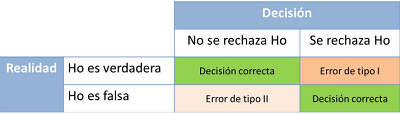
\includegraphics[width=7cm,height=2cm]{figuras/tipos_error.png}
\caption{Decisiones y tipos de error.}
\label{fig:decision}
\end{figure}
La probabilidad de ``Error tipo I" se denota por $\alpha$ y se denomina nivel de significación:
\begin{center}
$P(\mbox{``Error tipo I}") = P(\mbox{Rechazar } H_0|H_0 \mbox{ es cierta}) =\alpha$
\end{center}
El nivel de significación consiste en la probabilidad de rechazar la hipótesis nula $H_0$ cuando verdaderamente
es cierta. Este valor $\alpha$ es un parámetro que debe seleccionar la persona que quiere realizar un test
estadístico en base a cuán importante es rechazar $H_0$ cuando es cierta. Normalmente es del 5\%, lo
que implicará que 5 de cada 100 veces se acepta la hipótesis alternativa cuando la cierta es la hipótesis nula.
Cuanto menor sea el nivel de significación, cada vez es más difícil rechazar la hipótesis nula. Es decir, si
queremos equivocarnos menos veces, necesitamos mucha más evidencia para justificar el rechazo. Si es grande es
más fácil aceptar la hipótesis alternativa cuando en realidad es falsa.
\\Por otra parte, la probabilidad de ``Error tipo II" se denota por $\beta$:
\begin{center}
$P(\mbox{``Error tipo II}") = P(\mbox{Aceptar } H_0|H_0 \mbox{ es falsa}) =\beta$
\end{center}
Este error $\beta$ consiste en la probabilidad de aceptar la hipótesis nula $H_0$ cuando verdaderamente es
falsa.
\\Por último, cabe destacar el concepto de ``Potencia".
\begin{center}
$P(\mbox{``Potencia}") = P(\mbox{Rechazar } H_0|H_0 \mbox{ es falsa}) =1-\beta.$
\end{center}
La potencia es la probabilidad de detectar que una hipótesis es falsa. Los test estadísticos o pruebas de hipótesis
implementados en el presente proyecto se caracterizan por su potencia, siendo esta fija, y dejando como parámetro
libre el nivel de significación. Así, cuanto mayor es el nivel de potencia, mejor será el test, ya que se rechazarán
más hipótesis nulas cuando se deben rechazar (mayor habilidad en aceptar correctamente hipótesis alternativas).

En este proyecto se pondrá el énfasis en el nivel de significación, ya que es la hipótesis alternativa la que se
quiere probar y no se quiere aceptar si en realidad no es cierta es decir, si aceptamos la hipótesis alternativa
queremos equivocarnos con un margen de error muy pequeño. Obviamente, lo ideal sería que tanto $\alpha$ como
$\beta$ fuesen nulos y que no se cometiese ningún error, o que ambos valores fuesen muy pequeños. Como no se pueden
disminuir ambos errores a la vez, se controla el ``Error tipo I".

%***************************************************************************************************************************

\section{Intervalos de confianza}
El nivel de significación fijado divide en dos regiones el conjunto de posibles valores del estadístico de
contraste: la región de aceptación y la región de rechazo o región crítica. Se denomina región de aceptación
a la región que conduce a la aceptación de $H_0$ y región de rechazo a la región que conduce al rechazo de $H_0$
en favor de $H_1$. Aquí surge el concepto de \textbf{Cola}, que indica la porción o porciones de una distribución
de probabilidad en la cual se rechaza la hipótesis nula, es decir, la \textbf{región de rechazo}.

La determinación de las regiones de aceptación o de rechazo depende de cómo se establezca la hipótesis
alternativa $H_1$. Por ejemplo, si hablamos de un contraste en el que se esté contrastando una determinada
media ($\mu_0$) se podría establecer como $H_1$ que la media en realidad sea menor, mayor o distinta a
($\mu_0$):\\\\
\begin{itemize}
\item Media menor (test unilateral con cola a la izquierda):
\end{itemize}
\begin{center}
$H_0: \mu = \mu_0$
\\$H_1: \mu < \mu_0$
\end{center}
\begin{itemize}
\item Media mayor (test unilateral con cola a la derecha):
\end{itemize}
\begin{center}
$H_0: \mu = \mu_0$
\\$H_1: \mu > \mu_0$
\end{center}
\begin{itemize}
\item Media distinta (test bilateral o de dos colas):
\end{itemize}
\begin{center}
$H_0: \mu = \mu_0$
\\$H_1: \mu \neq \mu_0$
\end{center}
En la figura \ref{fig:intervalos_normal}, podemos ver cómo quedarían establecidos los intervalos para el ejemplo. En
rojo se muestra la región de rechazo:
\begin{figure}[h]
\centering
\subfigure[Test unilateral. Cola a la izquierda.]{
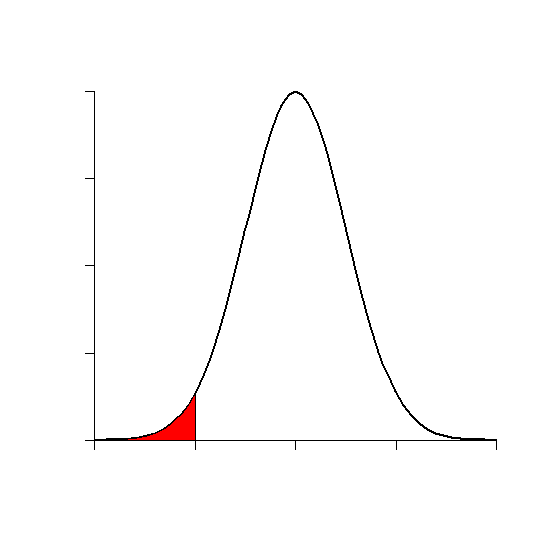
\includegraphics[width=5cm,height=3cm]{figuras/test_unilateral_izq.png} }
\subfigure[Test unilateral. Cola a la derecha.]{
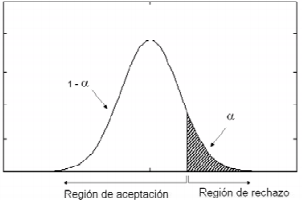
\includegraphics[width=5cm,height=3cm]{figuras/test_unilateral_der.png} }
\end{figure}
\begin{figure}[h]
\centering
\subfigure[Test bilateral o de dos colas.]{
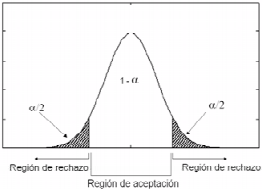
\includegraphics[width=5cm,height=3cm]{figuras/test_bilateral.png} }
\caption{Regiones de aceptación y rechazo.}
\label{fig:intervalos_normal}
\end{figure}

Como se puede observar en el caso del test bilateral o de dos colas, el $\alpha$ se divide en dos porciones iguales:
$\alpha / 2$, que constituyen la región de rechazo. La región de aceptación tendrá en todos los casos probabilidad
$1 - \alpha$.

%***************************************************************************************************************************

\section{Decisión final y \textit{\textit{p-valor}}} \label{pvalor}
Si el valor del estadístico cae en la región de aceptación, se acepta la hipótesis nula, ya que no existen
razones suficientes para rechazar $H_0$ con el nivel de significación dado. Por tanto, en este caso se diría
que el contraste es estadísticamente no significativo, es decir, no existe evidencia estadísticamente significativa
en favor de $H_1$.
\begin{figure}[h]
\centering
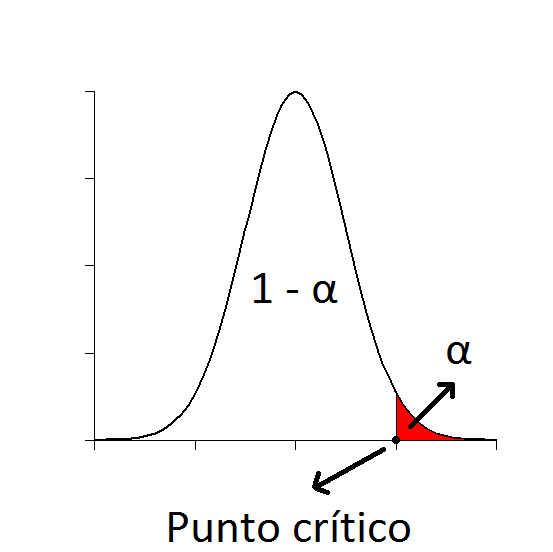
\includegraphics[width=5cm,height=3cm]{figuras/critico.png}
\caption{Punto crítico.}
\label{fig:punto_critico}
\end{figure}
La figura \ref{fig:punto_critico} nos muestra el punto crítico: si el estadístico obtenido por el test o
prueba de hipótesis es 5 y el punto crítico es 4.5, se rechaza $H_0$ ya que el estadístico pertenece a la
región de rechazo.

La decisión de rechazar o aceptar la hipótesis nula, se puede determinar también mediante el $\textit{p-valor}$,
que es el parámetro utilizado para realizar los test estadísticos en este proyecto. El $\textit{p-valor}$ proporciona
un forma más eficiente de determinar si el contraste es o no estadísticamente significativo, ya que no sería
necesario recalcular regiones de aceptación y rechazo cada vez que el usuario de los test cambia de nivel de
significación.

\begin{center}
``El $\textit{p-valor}$, es la probabilidad que hay de obtener un valor al menos tan extremo como el estadístico en cuestión
que se ha calculado."
\end{center}

Para entender mejor el concepto de $\textit{p-valor}$, conviene hablar de las distribuciones de probabilidad vistas en la
figura \ref{fig:pdf} de la sección \ref{estadistico} donde se hablaba del estadístico de contraste. Estas
distribuciones son funciones que se denominan ``funciones de densidad de probabilidad" (FDP). Como expusimos en
la sección \ref{estadistico}, estas funciones proporcionan la probabilidad que existe para cada valor
diferente del estadístico (cuán probable es obtener ese valor del estadístico). Si, en vez de trabajar con las
funciones de densidad de probabilidad, se trabaja con las funciones de distribución acumuladas (FDA), para cada
valor del estadístico éstas devolverían la probabilidad de obtener un valor igual o menor que ese estadístico siendo
la hipótesis nula cierta. En la figura \ref{fig:comparativa_pdf_cdf} podemos ver una comparación entre los dos
tipos de funciones para el caso de la distribución $\chi^2$:

\begin{figure}[h]
\centering
\subfigure[Función de densidad de probabilidad.]{
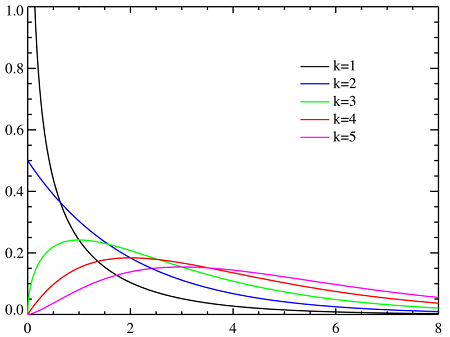
\includegraphics[width=5cm,height=3cm]{figuras/pdf_chi_cuadrado.png} }
\subfigure[Función de distribución acumulada.]{
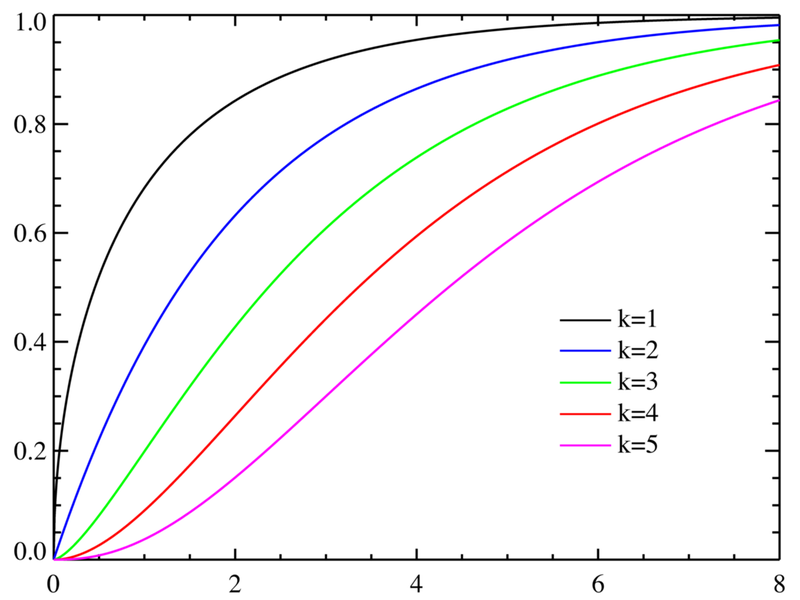
\includegraphics[width=5cm,height=3cm]{figuras/cdf_chi_cuadrado.png} }
\caption{Comparativa entre FDP y FDA.}
\label{fig:comparativa_pdf_cdf}
\end{figure}

Visto de otro modo, con la distribución acumulada, dado un estadístico, nos devuelve la probabilidad que hay de
obtener un valor al menos tan extremo como el estadístico en cuestión. Esto es el \textbf{$\textit{p-valor}$}. Por ejemplo si
el valor del estadístico es 3 y el test da como resultado un $\textit{p-valor}$ igual a 0.1, esto quiere decir que un 10\% de
las veces vamos a obtener un valor similar. Si el $\textit{p-valor}$ es muy bajo, es decir, la probabilidad de obtener un valor
al menos tan extremo como ese estadístico es muy baja, se puede concluir que la hipótesis nula no es cierta, ya que
sería poco probable que siendo cierta se obtuviese ese estadístico.

El criterio para saber si el $\textit{p-valor}$ es lo suficientemente bajo como para rechazar que la hipótesis nula sea cierta
es tomado de acuerdo al nivel de significancia establecido. Como se ha mencionado en la sección \ref{tipos_error}, el
nivel de significancia o $\alpha$ indica la probabilidad de rechazar la hipótesis nula siendo ésta cierta. Si el
$\textit{p-valor}$ es menor que el nivel de significancia se rechaza la hipótesis nula.

Según se disminuye $\alpha$, cada vez es más difícil de rechazar la hipótesis nula, ya que se necesita mucha más
evidencia para justificar el rechazo. Por ejemplo, si $\alpha$ es 0.05 y la probabilidad de obtener un estadístico
igual a 1 es 0.03, se rechaza la hipótesis nula. Sin embargo, si el $\alpha$ fuese 0.01, no se podría rechazar: no hay suficiente evidencia de que la hipótesis nula sea falsa.

%***************************************************************************************************************************

\section{Etapas en la resolución de un contraste de hipótesis}
En un contraste de hipótesis siempre se siguen una serie de pasos definidos. Como se ha ido viendo a lo largo
del capítulo, los pasos para la realización de una prueba de hipótesis o test estadístico son los siguientes
\cite{libro}:
\begin{enumerate}
\item Especificación de la hipótesis nula $H_0$ y de la hipótesis alternativa $H_1$.
\item Suponer que $H_0$ es verdadera (el test sirve para que a partir de la muestra de datos podamos rechazar
$H_0$ en beneficio de $H_1$).
\item Calcular un estadístico de prueba o estadístico de contraste. Este estadístico se usa para evaluar la
fuerza de la evidencia en contra de $H_0$ (medir la discrepancia entre la hipótesis y la muestra).
\item Establecer un nivel de significación $\alpha$ en base a cómo de importante se considere rechazar $H_0$
cuando realmente es verdadera.
\item El nivel de significación fijado divide en dos regiones el conjunto de posibles valores del estadístico
de contraste: la región de aceptación y la región de rechazo o región crítica.
\item Si el valor del estadístico cae en la región de rechazo, se rechaza la hipótesis nula, ya que esto
evidencia que los datos obtenidos de la muestra no son compatibles con $H_0$. Por tanto, en este caso se diría
que el contraste es estadísticamente significativo, es decir, existe evidencia estadísticamente significativa en
favor de $H_1$.
\item Si el valor del estadístico cae en la región de aceptación, se acepta la hipótesis nula, ya que no existen
razones suficientes para rechazar $H_0$ con el nivel de significación dado. Por tanto, en este caso se diría
que el contraste es estadísticamente no significativo, es decir, no existe evidencia estadísticamente significativa
en favor de $H_1$.
\item La decisión de rechazar o aceptar la hipótesis nula, se puede determinar también mediante el $\textit{p-valor}$,
que es el parámetro utilizado para realizar los test estadísticos en este proyecto. El $\textit{p-valor}$ proporciona
un forma más eficiente de determinar si el contraste es o no estadísticamente significativo, ya que no sería
necesario recalcular regiones de aceptación y rechazo cada vez que el usuario de los test cambia de nivel de
significación.
\end{enumerate}

%***************************************************************************************************************************

\section{Tests paramétricos} \label{parametricos}
Uno de los tipos más comunes de test son los test paramétricos. En general, estos test son más robustos y
tienen mayor potencia que los test no paramétricos, que se verán más adelante en la sección \ref{no_parametricos}.
Sin embargo, las pruebas paramétricas se basan en supuestos que muy probablemente se violan cuando se analiza el
rendimiento de algoritmos de optimización y minería de datos \cite{parametricos}. Estas suposiciones
o condiciones paramétricas que deben cumplir los resultados de los algoritmos son explicadas a continuación.

%----------------------------------

\subsection{Condiciones Paramétricas} \label{condiciones}

\subsubsection{Independencia}
En estadística, dos eventos son independientes si cuando uno de ellos se da no modifica la probabilidad de la
ocurrencia del otro. Dicho de otra forma: cuando las muestras o datos obtenidos por los algoritmos, es decir los
resultados de éstos, no dependen unos de otros. La independencia es una característica que en este proyecto debe
asumir el usuario de los test, y, por tanto, podrá actuar de una forma u otra bajo su responsabilidad.

\subsubsection{Normalidad}
Una muestra u observación es normal cuando su comportamiento sigue una distribución normal (o distribución de
Gauss) con una cierta media $\mu$ y varianza $\sigma^2$. En la figura \ref{fig:normalidad} podemos ver que a la
izquierda se cumple el supuesto de normalidad, mientras que a la derecha los datos de la muestra no están distribuidos
de forma normal:

\begin{figure}[h]
\centering
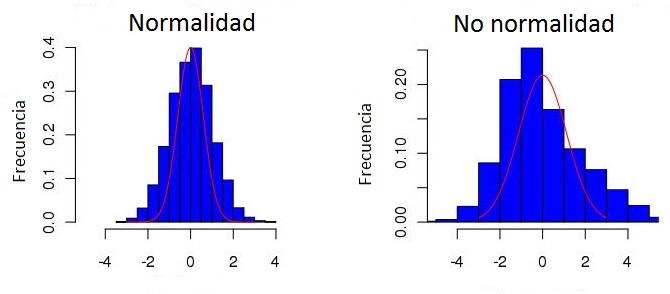
\includegraphics[width=9cm,height=3cm]{figuras/normalidad.jpg}
\caption{Normalidad vs. No normalidad.}
\label{fig:normalidad}
\end{figure}

En este proyecto se pueden realizar los siguientes test no paramétricos para comprobar el supuesto de normalidad:

\begin{itemize}
\item \textbf{Shapiro–Wilk:} contrasta la hipótesis nula de que las muestras o poblaciones provienen de una
población normalmente distribuida. Analiza la muestra para hallar el nivel de simetría y Kurtosis (forma de
la curva) para calcular la diferencia con respecto a una distribución normal, obteniendo el \textit{p-valor} de la suma
de los cuadrados de estas discrepancias. Se considera de los más potentes, sobre todo para muestras de menos
de 30 elementos. Sin embargo, el rendimiento de esta prueba se ve afectado de forma negativa cuando no existe
independencia en los datos.
\item \textbf{D’Agostino–Pearson:} contrasta la hipótesis nula de que las muestras o poblaciones provienen de
una población normalmente distribuida. Primero calcula el coeficiente de asimetría (en qué medida la normal es
simétrica ó coeficiente 0) y el coeficiente de Kurtosis (grado de amplitud, donde lo normal es coeficiente 0) para
cuantificar cuán lejos se está de la distribución normal. Luego, calcula cuánto difiere cada uno de los valores
de los esperados en una distribución normal, para obtener el $\textit{p-valor}$ de la suma de estas discrepancias.
Es menos potente que el test de Shapiro-Wilk, pero no se ve afectado cuando los datos no son independientes.
\item \textbf{Kolmogorov–Smirnov:} realiza una prueba de bondad de ajuste, para determinar si los datos observados
de la muestra se ajustan a la distribución normal. Tiene como $H_0$ que la distribución obtenida de los datos
observados es idéntica a la distribución normal. Es la prueba que menos potencia presenta de los tres, y por tanto
es la que peor funciona.
\end{itemize}

\subsubsection{Homocedasticidad}
La homocedasticidad es la condición que dice que las poblaciones de entrada o datos obtenidos por los algoritmos
proceden de poblaciones con varianzas iguales. Es decir, esta propiedad indica la hipótesis de igualdad de
varianzas. El caso contrario sería heterocedasticidad. En la figura \ref{fig:homocedasticidad} se puede apreciar
la diferencia existente entre unos datos que presentan homocedasticidad y otros que no, donde el eje de ordenadas
representa la varianza del error (la varianza dentro de cada tratamiento o la varianza de los resultados obtenidos
por un algoritmo en los distintos conjuntos de datos), y el eje de abscisas representa a las observaciones. En el
primer caso, la varianza del error se mantiene constante a lo largo de las observaciones, mientras que en el otro
caso no:

\begin{figure}[h]
\centering
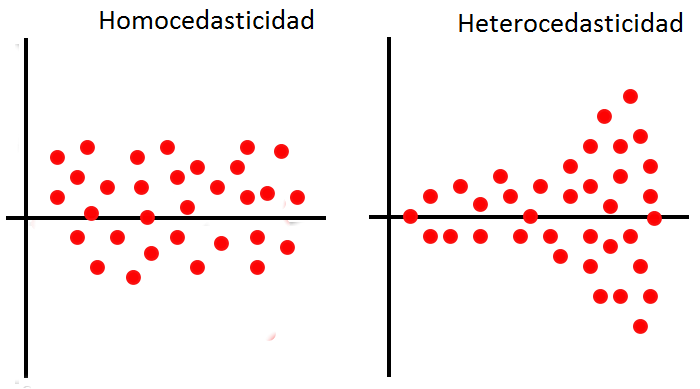
\includegraphics[width=6cm,height=3cm]{figuras/homocedasticidad.png}
\caption{Homocedasticidad vs. Heterocedasticidad.}
\label{fig:homocedasticidad}
\end{figure}

En este proyecto se puede realizar el siguiente test no paramétrico para comprobar el supuesto de homocedasticidad:

\begin{itemize}
\item \textbf{Test de Levene:} contrasta la hipótesis nula de que todas las poblaciones de entrada proceden de
poblaciones con varianzas iguales. Se utiliza para comprobar si K muestras pertenecientes a datos obtenidos por
K algoritmos presentan o no homogeneidad de varianzas. 
\end{itemize}

%----------------------------------

\subsection{Test ANOVA}
El análisis de la varianza (ANOVA) es uno de los test estadísticos más ampliamente utilizados para probar
la igualdad de más de dos medias de la población. Se trata de una versión más general del t-test, ya que permite
comparar más de 2 poblaciones (en este proyecto resultados de más de dos algoritmos). Dado que es un test
paramétrico, se asume que se dan las condiciones de independencia, normalidad y homocedasticidad en su
aplicación. De no ser el caso, los resultados de esta prueba no son fiables.

\subsubsection{Hipótesis}
\begin{itemize}
\item Hipótesis nula $H_0$: $\mu_1 = \mu_2 = \mu_3 ... = \mu_K$.
\item Hipótesis alternativa $H_1$: $\exists \quad \mu_j \neq \mu \quad j=1,2,...,K$.
\end{itemize}
La hipótesis nula indica que las medias de distintas poblaciones o muestras coinciden $(K>2)$, frente a la
hipótesis alternativa de que por lo menos una de las poblaciones tiene una media que difiere de las demás. Es,
por tanto, un contraste o prueba unilateral con cola a la derecha. En este proyecto el parámetro $K$ viene
determinado por el número de algoritmos que existen en la muestra de datos.

\subsubsection{Pasos a desarrollar}
Los pasos a seguir para realizar el test de ANOVA son los siguientes:
\begin{itemize}
\item Se analiza la variación total (respecto a la media general o media de medias de los resultados de cada
algoritmo):
\[ variacion_t = \sum_{i=1}^{N} \sum_{j=1}^{K} (X_{ij} - \bar{X})^2, \]
donde $\bar{X}$ es la media general, $N$ es el número de conjuntos de datos o problemas sobre los que se
aplican los algoritmos y $X_{ij}$ es un resultado específico obtenido por un algoritmo.
\item Se halla también la variación entre los diferentes tratamientos o algoritmos (efecto de la media de cada
tratamiento respecto a la media general):
\[ variacion_{tr} = \sum_{i=1}^{K} N (\bar{X}_i - \bar{X})^2, \]
donde $\bar{X}_i$ representa la media del tratamiento o algoritmo.
\item La variación dentro del tratamiento o variación del error (cada valor respecto a la media de su tratamiento):
\[ variacion_e = \sum_{i=1}^{N} \sum_{j=1}^{K} (X_{ij} - \bar{X}_{j})^2, \]
donde $\bar{X}_{j}$ representa la media de un tratamiento o algoritmo.
\item Se calculan los grados de libertad totales, del tratamiento y del error como:
\[ GLT = (NK)-1 \]
\[ GLTR = K-1 \]
\[ GLE = GLT - GLTR \]
\item Luego se determinan los cuadrados medios totales ($CMT$) del tratamiento ($CMTR$) y del error ($CME$),
que son las variaciones divididas entre los grados de libertad correspondientes.
\item Se halla el estadístico, que se distribuye como una distribución $\mathcal{F}$ con $K-1$ y $(KN)-K$ grados de libertad:
\[ anova = CMT / CME \]
\item Por último se halla el $\textit{p-valor}$ y se toma la decisión en función del nivel de significancia. A modo
de ejemplo para el cálculo del $\textit{p-valor}$ en este caso, primero se haya la probabilidad de obtener un
estadístico menor o igual que el calculado previamente (es decir, el valor que proporciona la función de distribución acumulada $\mathcal{F}$ de Fisher-Snedecor para el estadístico con $K-1$ y $(KN)-K$ grados de libertad, como vimos en
la sección \ref{pvalor}). Esto representaría un área (probabilidad acumulada) en la función de densidad de
probabilidad: el área a la izquierda del valor del estadístico. Dado que se trata de un contraste unilateral con cola
a la derecha, se resta esta probabilidad a la probabilidad total, es decir, a 1, para obtener así el área que queda a la derecha del estadístico. Si este valor resultante ($\textit{p-valor}$) es menor que el nivel de significancia, se
rechazaría la hipótesis nula.

En un contraste bilateral, para hallar el $\textit{p-valor}$ habría que multiplicar el valor devuelto en la función de distribución acumulada por 2, ya que en este caso habría dos colas.
\end{itemize}

%----------------------------------

\subsection{t-test}
El caso más simple de ANOVA donde intervienen únicamente 2 muestras o algoritmos es realizado por este test, también
conocido como la prueba $\mathcal{T}$ de Student. Dado que es un test paramétrico, se asume que se dan las condiciones
de independencia, normalidad y homocedasticidad en su aplicación. De no ser el caso, los resultados de esta prueba no
son fiables.

\subsubsection{Hipótesis}
\begin{itemize}
\item Hipótesis nula $H_0$: $\mu_1 = \mu_2$.
\item Hipótesis alternativa $H_1$: $\mu_1 \neq \mu_2$.
\end{itemize}
La hipótesis nula indica que las medias de las 2 poblaciones o muestras coinciden, frente a la hipótesis alternativa
de que son distintas. Se trata, por tanto, de un contraste o prueba bilateral. El estadístico de este test, sigue una distribución $\mathcal{T}$ de Student con $2N-2$ grados de libertad.

%----------------------------------

%***************************************************************************************************************************

\section{Tests no paramétricos} \label{no_parametricos}
Cuando los datos obtenidos de la aplicación de los algoritmos de aprendizaje automático no cumplen las
características de independencia, normalidad u homocedasticidad total o parcialmente,  es necesario aplicar
test no paramétricos. La validación de nuevos algoritmos requiere con frecuencia la definición de un marco
experimental exhaustivo y la parte crítica de estas comparaciones recae en la validación estadística de los
resultados, contrastando las diferencias encontradas entre métodos. Dentro de las técnicas disponibles, destacan
los test no paramétricos debido a su flexibilidad y a las pocas restricciones de uso que presentan (a diferencia
de los test paramétricos, los cuales sufren a menudo problemas derivados de la imposibilidad de cumplir las
condiciones paramétricas para su uso) \cite{no_parametricos}.

%----------------------------------

\subsection{Test de Wilcoxon}
La prueba de los rangos con signo de Wilcoxon también conocida como el test de Wilcoxon es una prueba no
paramétrica que se utiliza como alternativa a la prueba $\mathcal{T}$ de Student cuando no se puede suponer la normalidad
de las muestras. Es, por tanto, menos potente que que la prueba $\mathcal{T}$ de Student. El test de Wilcoxon fue creado
por Frank Wilcoxon y publicado en 1945 \cite{wilcoxon}.

Sirve para comparar dos métodos o tratamientos (en este proyecto interesa comparar dos algoritmos). Por tanto,
los individuos (los problemas) donde se aplican los algoritmos tienen que ser los mismos. Es decir, a un mismo
individuo se le efectúa la medición de dos variables: las muestras son apareadas. Para tomar la decisión hay
que basarse en las observaciones de N individuos independientes (sin relación existente entre ellos). Para tamaños
muestrales pequeños, se puede determinar mediante la comparación del estadístico con el valor crítico de la
tabla de Wilcoxon. Para tamaños muestrales grandes ($> 25$), el test se puede aproximar con la distribución normal.

\subsubsection{Hipótesis}
\begin{itemize}
\item Hipótesis nula $H_0$: la mediana de las diferencias $ = 0$.
\item Hipótesis alternativa $H_1$: la mediana de las diferencias $ \neq 0$.
\end{itemize}
La mediana, es el valor que ocupa el lugar central de todos los datos cuando éstos están ordenados de menor a
mayor. $H_0$ indica que la mediana de las diferencias de dos muestras (resultados de dos algoritmos) relacionadas
son iguales, es decir, las dos medianas son iguales (los resultados obtenidos no dependen del algoritmo).
$H_1$ indica, por otra parte, que las medianas son diferentes. Se trata, por tanto, de una prueba bilateral.

\subsubsection{Pasos a desarrollar}
Los pasos a seguir para realizar la prueba de los rangos de Wilcoxon son los siguientes:
\begin{itemize}
\item Se calculan las diferencias entre las muestras. Por ejemplo: diferencias entre los resultados del algoritmo
A y B.
\subitem - Se eliminan los elementos que tengan diferencias nulas.
\item Se ordenan las diferencias en valor absoluto (independientemente del signo).
\item Se asignan rangos de orden 1,2,...,N. Si hay empates se calcula la media del rango de cada uno de los elementos
repetidos.
\item Suma de los rangos según los signos que tengan las diferencias para obtener los estimadores:
\subitem - $T(+) = $ Suma de los rangos correspondientes a diferencias positivas. 
\subitem - $T(-) = $ Suma de los rangos correspondientes a diferencias negativas.
\item Definir el estadístico:
\subitem - $T = \min [T(+), T(-)]$
\item Si $N \leq 25$, se examina la tabla de Wilcoxon que nos da los valores críticos (el intervalo de aceptación)
para cada valor de N y cada nivel de significancia. El contraste será estadísticamente significativo si: 
$T <= $ límite inferior correspondiente.
\item Si $N > 25$, el estadístico se ajusta a la distribución normal. Por tanto, se calcula el estadístico $Z$ y
se toma la decisión en función del $\textit{p-valor}$ y del nivel de significancia:
\[ Z = \frac{T-\frac{N(N+1)}{4}}{\sqrt{\frac{N(N+1)(2N+1)}{24}}} \]
\end{itemize}

%----------------------------------

\subsection{Test de Friedman}
El test de Friedman es una prueba no paramétrica que puede realizar comparaciones entre dos o más algoritmos, es
decir, se trata de una prueba de comparaciones múltiples. Fue desarrollada por el economista Milton Friedman y
trabaja asignando rankings para establecer cuál es el mejor algoritmo de la muestra de datos proporcionada.

\subsubsection{Hipótesis}
\begin{itemize}
\item Hipótesis nula $H_0$: no existen diferencias entre los algoritmos.
\item Hipótesis alternativa $H_1$: existen diferencias entre los algoritmos.
\end{itemize}
La hipótesis nula quiere decir que todos los algoritmos se comportan de la misma forma, por lo que los rankings
que poseen deben de ser similares. La hipótesis alternativa, por el contrario, afirma que existen diferencias,
lo cual quiere decir que, al menos, el rendimiento de un algoritmo es diferente al rendimiento que presentan los
demás. Se trata, por tanto, de un contraste o prueba unilateral con cola a la derecha.

\subsubsection{Pasos a desarrollar}
Los pasos a seguir para realizar el test de Friedman son los siguientes:
\begin{itemize}
\item En primer lugar se asignan rankings $r_{ij}$ a los resultados obtenidos por cada algoritmo $j$ en cada
problema $i$. Es decir, para cada problema o conjunto de datos se asigna un ranking cuyos valores están
comprendidos entre $1$ y $K$, donde $K$ representa el número de algoritmos que se están comparando. Los rankings
se asignan de forma ascendente (1 al mejor resultado, 2 al segundo mejor, etc.) y se tiene en cuenta la función
objetivo de los algoritmos, es decir, si lo que se pretende es minimizar o maximizar resultados.
\item En caso de que haya empates en la asignación de rankings anterior, se asignan rankings medios:
\[ r_{ij} = \frac{rep + (2pos) + 1}{2}, \]
donde $rep$ representa el número de veces que se repite el dato y $pos$ representa la posición que ocupa
el dato repetido.
\item A continuación, se calculan los rankings medios de cada algoritmo en los $N$ problemas:
\[ R_j = \frac{\sum_{i=1}^{N} r_{ij}}{N} \]
\item El estadístico de Friedman sigue una distribución $\chi^2$ con $K-1$ grados de
libertad:
\[ friedman = \frac{12N}{K(K+1)} \left[\sum R_j^2 - \frac{K(K+1)^2}{4} \right] \]
\item Por último se halla el $\textit{p-valor}$ y se toma la decisión en función del nivel de significancia.
\end{itemize}

%----------------------------------

\subsection{Test de Iman-Davenport}
El estadístico de Friedman fue mejorado por Iman y Davenport, que demostraron que tenía un comportamiento
demasiado conservador (se tiende a aceptar la hipótesis nula y, por tanto, la potencia del test es menor).

\subsubsection{Hipótesis}
\begin{itemize}
\item Igual al test de Friedman.
\end{itemize}

\subsubsection{Pasos a desarrollar}
\begin{itemize}
\item El test de Iman-Davenport hace las mismas operaciones que el test de Friedman pero en él se calcula
un estadístico más ajustado (en el que también interviene el estadístico de Friedman). Este nuevo estadístico,
sigue una distribución $\mathcal{F}$ con $(K-1)$ y $(K-1)*(N-1)$ grados de libertad, donde $N$
representa el número de problemas o conjuntos de datos y $K$ el número de algoritmos:
\[ iman_d = \frac{(N-1)friedman}{N(K-1)-friedman} \]
\end{itemize}

%----------------------------------

\subsection{Test de los Rangos Alineados de Friedman}
El test de los rangos alineados de Friedman realiza comparaciones y asigna rankings teniendo en cuenta a
todos los conjuntos de datos, a diferencia del test de Friedman, que asigna rankings dentro de cada conjunto
(es decir, dentro de los resultados obtenidos por los algoritmos para cada problema en particular). Por tanto,
en este caso los valores de los rankings irán desde $1$ hasta $K*N$. Suele emplearse cuando el número de
algoritmos en la comparación es pequeño y cuando se quiere realizar una comparación entre conjuntos de datos.

\subsubsection{Hipótesis}
\begin{itemize}
\item Igual al test de Friedman.
\end{itemize}

\subsubsection{Pasos a desarrollar}
\begin{itemize}
\item Cálculo de las observaciones alineadas: primero se halla el valor de localización, que es el rendimiento
medio alcanzado por los algoritmos en cada conjunto de datos y luego se calculan las diferencias entre el
rendimiento obtenido por cada algoritmo con respecto al valor de localización dentro de un mismo conjunto de
datos.
\item Se repite el primer paso para los $N$ conjuntos de datos.
\item Se juntan todas las observaciones alineadas y se ordenan para asignar los rankings alineados desde $1$
hasta $K*N$. En caso de empates se procede asignando valores medios igual que en el test de Friedman.
\item Se calculan los rankings medios de cada algoritmo en los $N$ problemas.
\item El estadístico para esta prueba sigue una distribución $\chi^2$ con $K-1$ grados de
libertad:
\[ rangos_{al} = \frac{(K-1) \left[ \sum_{j=1}^{K} \hat{R_{j}^{2}} - (\frac{KN^2}{4})(KN+1)^2 \right]}
{\left[\frac{KN(KN+1)(2KN+1)}{6}\right] - (\frac{1}{K}) \sum_{i=1}^{N} \hat{R_{i}^{2}}}, \]
donde $\hat{R_{i}}$ y $\hat{R_{j}}$ son la suma total de los rankings del problema $i$ y del algoritmo $j$
respectivamente.
\item Por último se halla el $\textit{p-valor}$ y se toma la decisión en función del nivel de significancia.
\end{itemize}

%----------------------------------

\subsection{Test de Quade}
El test de Quade tiene en cuenta, a diferencia del test de Friedman que considera que todos los problemas son
iguales en importancia, que algunos problemas son más difíciles o que los resultados que obtienen los algoritmos
sobre ellos son más distantes (se realiza una ponderación).

\subsubsection{Hipótesis}
\begin{itemize}
\item Igual al test de Friedman.
\end{itemize}

\subsubsection{Pasos a desarrollar}
\begin{itemize}
\item Se obtienen los rankings de cada conjunto de datos de la misma forma que en Friedman.
\item Asignación de rankings a los problemas en función del tamaño del rango de la muestra en cada
uno (diferencia entre el valor observado más alto y el más bajo). Este ranking de $1$ a $N$ usa también
rankings medios en caso de empate.
\item A partir de estos datos se pueden obtener los rankings medios finales para cada algoritmo y obtener
el estadístico, que sigue como una distribución $\mathcal{F}$ con $(K-1)$ y $(K-1)*(N-1)$ grados de libertad.
\item Por último se halla el $\textit{p-valor}$ y se toma la decisión en función del nivel de significancia.
\end{itemize}

%----------------------------------

\subsection{Tests POST-HOC}
Los test no paramétricos de ranking (test de Friedman, Iman-Davenport, Rangos Alineados de Friedman y Quade),
dan como resultado la existencia o no de diferencias significativas entre los algoritmos sobre los que se han
aplicado. Es decir, nos dice si el contraste de hipótesis es o no estadísticamente significativo. Si se rechaza
la hipótesis nula de ``todos los algoritmos son iguales", sabremos que entre los algoritmos existen diferencias.
Sin embargo, puede ocurrir que un algoritmo presente un rendimiento similar a otro u otros y por tanto se pueda
considerar igual.

Estos test comparan los algoritmos y realizan contrastes de hipótesis entre ellos para determinar diferencias.

\subsubsection{Hipótesis}
\begin{itemize}
\item Hipótesis nula $H_0$: el algoritmo $i$ y $j$ son iguales.
\item Hipótesis alternativa $H_1$: el algoritmo $i$ y $j$ son distintos.
\end{itemize}
Se trata, por tanto, de test que realizan contrastes bilaterales, ya que están destinados a encontrar diferencias
a posteriori en caso de que el test de ranking sea estadísticamente significativo. Se distinguen dos tipos de
comparación:

\begin{itemize}
\item Método de control: se compara el primer algoritmo del ranking devuelto por el test de ranking con el resto
de algoritmos y por tanto habrá $K-1$ comparaciones o contrastes.
\item Comparación múltiple: compara todos los algoritmos entre sí. El número de comparaciones o contrastes por
tanto es:
\[ m = \frac{K(K-1)}{2} \]
\end{itemize}

Todos los test POST-HOC aproximan los valores Z (estadísticos) de una distribución normal a partir de las
diferencias entre dos rankings. La forma de aproximar estos valores $Z$ varía en función del test de ranking de
donde se provenga:

\begin{itemize}
\item Test de Friedman / Iman-Davenport:
\[ Z = \frac{(R_i - R_j)}{\sqrt{\frac{K(K+1)}{6N}}}, \]
donde $R_i$ y $R_j$ son los rankings medios obtenidos por el algoritmo $i$ y $j$ respectivamente en el test
de Friedman.
\item Test de los Rangos Alineados de Friedman:
\[ Z = \frac{\hat{R_{i}} - \hat{R_{j}}}{\sqrt{\frac{K(K+1)}{6N}}}, \]
donde $\hat{R_{i}}$ y $\hat{R_{j}}$ son los rankings medios obtenidos por el algoritmo $i$ y $j$ respectivamente en el test
de los Rangos Alineados de Friedman.
\item Test de Quade:
\[ Z = \frac {T_i - T_j}{\sqrt{\frac{K(K+1)(2N+1)(K-1)}{18N(N+1)}}}, \]
donde $T_i$ y $T_j$ son los rankings medios obtenidos por el algoritmo $i$ y $j$ respectivamente en el test
de Quade.
\end{itemize}

Luego, calculan los $\textit{p-valor}es$ y ordenan todos los datos en función de éstos de mayor a menor 
significancia (de menor a mayor). El contraste de las hipótesis (los resultados), así como el cálculo del valor
$\alpha$ y los $\textit{p-valor}es$ ajustados varían en función de los test aplicados. Los $\textit{p-valor}es$
ajustados son $\textit{p-valor}es$ que dependen de toda la familia de comparaciones y no sólo de una comparación,
es decir, consideran la familia de hipótesis completa para cada pareja de algoritmos y se pueden comparar con el
nivel de significancia proporcionado sin ajustar.

\subsubsection{Tests}
\begin{itemize}
\item \textbf{Test de Bonferroni-Dunn:} el contraste de las hipótesis se realiza comparando cada $\textit{p-valor}$ con
el nivel de significancia ajustado:
\[ \alpha_{ajustado} = \frac{\alpha}{(K-1)} \]
\item \textbf{Test de Holm:} compara cada $\textit{p-valor}$ (empezando por el más significativo) con:
\[ \alpha_{ajustado_i} = \frac{\alpha}{(K-i)} \]
Si se rechaza una hipótesis continúa contrastando. En el caso de que una hipótesis se rechace se rechazan todas
las demás.
\item \textbf{Test de Finner:} compara cada $\textit{p-valor}$ (empezando por el más significativo) con:
\[ alpha_{ajustado_i} = 1-(1-\alpha)^{\frac{(K-1)}{i}} \]
Al igual que el test de Holm, si se rechaza una hipótesis continúa contrastando. En el caso de que una hipótesis
se rechace se rechazan todas
las demás.
\item \textbf{Test de Hochberg:} compara en la dirección opuesta a Holm. En el momento que encuentra una hipótesis
que pueda aceptar, acepta todas las demás.
\item \textbf{Test de Li:} rechaza todas las hipótesis si el $\textit{p-valor}$ menos significativo es menor que  $\alpha$.
En otro caso, acepta dicha hipótesis y rechaza cualquier hipótesis restante cuyo $\textit{p-valor}$ sea menor que un valor
específico:
\[ valor = \frac{(1-\textit{p-valor}_{k-1})}{(1-\alpha)\alpha} \]
\end{itemize}

Los test anteriores son para el caso de comparaciones simples (utilizan un método de control), con lo que
interviene el parámetro $K$ para realizar las $K-1$ comparaciones. Para el caso de comparación múltiple, habría
que reemplazar $K$ por $m$ (número de comparaciones múltiples). Para los test POST-HOC anteriores existe, por
tanto, un test POST-HOC de comparación múltiple que se obtiene de forma análoga, excepto para el test de Li. En
lugar del test de Li para comparaciones múltiples en este proyecto se implementa el test de Shaffer:

\begin{itemize}
\item \textbf{Test de Shaffer:} rechaza cada $H_i$ si:
\[ \textit{p-valor}_{i} \leq \frac{\alpha}{t_i}, \]
donde $t_i$ puede ser obtenido mediante:
\[ S(K) = \bigcup_{j=1}^{K} \{{j \choose 2}  + x: x \in S(K-j)\}, \]
que calcula la secuencia de número máximo de hipótesis que pueden ser ciertas en una comparación secuencial
entre $K$ distribuciones, donde $K \geq 2$ y $S(0) = S(1) = \{0\}$
\end{itemize}

Los test de la lista anterior están ordenados de menor a mayor potencia, siendo, como se puede apreciar,
el test de Bonferroni-Dunn el menos potente de todos y el test de Li el que mayor potencia presenta \cite{potencia}.

%----------------------------------

%***************************************************************************************************************************
\cleardoublepage
%***************************************************************************************************************************

\chapter{Análisis de requisitos}
El análisis de requisitos es el primer paso técnico del proceso de ingeniería del software. Es aquí donde se refina la declaración general del ámbito del software en una especificación concreta que se convierte en la base de todas las actividades de ingeniería del software que siguen.

En este proyecto, hemos utilizado el enfoque de metodología de desarrollo ágil Scrum \cite{libroscrum}. Los detalles de esta metodología y la razón de su utilización en este proyecto se detallan en la sección \ref{metodologia} del capítulo \ref{chgestion}. Para realizar el análisis de requisitos, a diferencia del enfoque de tradicional en el que los requisitos son descritos de una forma muy estricta y formal, esta metodología permite describir las necesidades del usuario de una manera más simple. Para ello, se establecen los requisitos mediante las \textbf{historias de usuario}. Las historias de usuario son requisitos escritos en un lenguaje coloquial bien directamente por el mismo cliente, o bien como un recordatorio posterior de las conversaciones mantenidas con el cliente. Consisten en una o dos frases en donde de una forma no precisa se detalla lo que el usuario requiere de la aplicación. Además, deben ser:

\begin{itemize}
\item \textbf{Independientes:} no depender de otras para su compleción.
\item \textbf{Negociables:} no son del todo claras, y por tanto se necesita discutir con los usuarios. Se concretan en los criterios de aceptación.
\item \textbf{Valoradas por el cliente:} esto permite conocer en qué está más interesado el cliente y qué es más importante para la aplicación.
\item \textbf{Estimables:} se puede establecer una valoración del tiempo que llevará completarlas.
\item \textbf{Pequeñas:} para poder hacer una mejor estimación. Normalmente más de 2 días y menos de 1 semana.
\item \textbf{Verificables:} se necesitan poder probar para saber si se ha completado con éxito. 
\end{itemize}

El formato a seguir es el siguiente:

\begin{center}
Como $<$tipo de usuario$>$, me gustaría $<$objetivo$>$, ya que $<$razón$>$
\end{center}

Además, a las historias de usuario se añaden criterios de aceptación y una prioridad.

Entre los beneficios de usar historias de usuario para elaborar los requisitos destaca que no se requiere elaborar una gran cantidad de documentos formales y por lo tanto se requiere menos tiempo para su administración. Por ello, permiten responder rápidamente a los requisitos cambiantes, algo a tener en cuenta sabiendo que normalmente los clientes o los usuarios finales con frecuencia no saben lo que necesitan desde un principio y es algo que se debe ir refinando a lo largo del proyecto.

Un nivel de abstracción mayor a las historias de usuario es dado por los denominados Epics. Los Epics son historias de usuario mucho más generales (a más alto nivel) que nos dan una primera idea del trabajo que puede estar involucrado en su definición. Los Epics se pueden desglosar en varias historias de usuario y están compuestos por un título o requerimiento muy general.

En este proyecto, primeramente se detallan los Epics y luego se describen las historias de usuario en las que se pueden desglosar. Para la prioridad de las historias de usuario, se han definido tres niveles en función del interés del cliente en las mismas:

\begin{itemize}
\item \textbf{Alta:} Indica que el cliente está muy interesado en el requerimiento en cuestión y que lo considera clave para la aplicación.
\item \textbf{Media:} Indica que el cliente está interesado en el requerimiento, pero no es tan importante para la aplicación. 
\item \textbf{Baja:} Indica aquellos requerimientos que, siendo favorables, son prescindibles.
\end{itemize}

%***************************************************************************************************************************

\section{Epics} \label{epics}
Los Epics son identificados mediante EP-x, donde x representa un número natural único.

\begin{itemize}
\item \textbf{EP-1:} Proporcionar una API REST de los test estadísticos.
\item \textbf{EP-2:} Permitir realizar test estadísticos paramétricos.
\item \textbf{EP-3:} Permitir realizar test estadísticos no paramétricos.
\item \textbf{EP-4:} Permitir realizar test estadísticos no paramétricos para evaluar las condiciones paramétricas.
\item \textbf{EP-5:} Permitir gestionar un fichero.
\item \textbf{EP-6:} Visualizar lo resultados de los test.
\item \textbf{EP-7:} Permitir modificar opciones de los test.
\item \textbf{EP-8:} Proporcionar una interfaz usable.
\end{itemize}

%***************************************************************************************************************************

\section{Historias de usuario}
Las historias de usuario se identifican mediante HU-x, donde x representa un número natural único. Cabe destacar que en este proyecto se consideran dos tipos de usuario: desarrollador y cliente. El primero, se considera debido a que una de las partes del proyecto consiste en desarrollar una API REST que hace disponible los test vía web. Esta API la puede utilizar un desarrollador para realizar la interfaz web, con lo que es necesario que un desarrollador diga las necesidades que requiere de la API. El cliente, por otra parte, se refiere al usuario final de la plataforma, es decir, el analista de datos que quiere validar algoritmos de aprendizaje automático. Ambos tienen intereses diferentes y por tanto se pueden considerar por separado.

% ----------------------------------------------------- %

\subsection{Historias de usuario desarrollador}

% *****************HISTORIA USUARIO 1****************** %

Desglosando el Epic \textbf{EP-1:} Proporcionar una API REST de los test estadísticos, se obtienen las siguientes historias de usuario:

\begin{table}[H]
	\begin{tabular}{| p{3cm}| p{11cm} |}
		\hline
		\multicolumn{2}{|c|}{\textbf{HU-1} - Acceder a test} \\ \hline
		\textbf{Como:} & Desarrollador \\ \hline
		\textbf{Me gustaría:} & acceder a los test como recursos independientes con parámetros opcionales. \\ \hline
		\textbf{Ya que:} & esto facilita su utilización y los hace más flexibles. \\ \hline
		\multirow{3}{11cm}{\textbf{C. Aceptación:}} & - Los test estadísticos son accesibles individualmente como un recurso. \\
		& - Los métodos de POST-HOC pueden ser también accedidos individualmente como un sub recurso dentro del recurso de acceso del test principal. \\
		& - Se proporcionan varias URIs (identificador de recursos uniforme) para cada test cuyos parámetros (como el nivel de significación, la función objetivo o el test POST-HOC) son opcionales, teniendo un valor común por defecto. \\ \hline
		\textbf{\textbf{Prioridad:}} & alta \\ \hline
	\end{tabular}
\end{table}

% *****************HISTORIA USUARIO 2****************** %

\begin{table}[H]
	\begin{tabular}{| p{3cm}| p{11cm} |}
		\hline
		\multicolumn{2}{|c|}{\textbf{HU-2} - Gestionar ficheros} \\ \hline
		\textbf{Como:} & Desarrollador \\ \hline
		\textbf{Me gustaría:} & poder gestionar un fichero como un recurso independiente. \\ \hline
		\textbf{Ya que:} & esto facilita la subida y consulta de ficheros. \\ \hline
		\multirow{2}{11cm}{\textbf{C. Aceptación:}} & - Los ficheros son accesibles individualmente como un recurso. \\
		& - Los recursos de fichero son creados de forma individual. \\ \hline 
		\textbf{\textbf{Prioridad:}} & alta \\ \hline
	\end{tabular}
\end{table}
	
% *****************HISTORIA USUARIO 3****************** %

\begin{table}[H]
	\begin{tabular}{| p{3cm}| p{11cm} |}
		\hline
		\multicolumn{2}{|c|}{\textbf{HU-3} - Devolver datos JSON} \\ \hline
		\textbf{Como:} & Desarrollador \\ \hline
		\textbf{Me gustaría:} & que los datos devueltos por los servicios de la API REST fuesen en formato JSON (JavaScript Object Notation). \\ \hline
		\textbf{Ya que:} & es un formato ligero para el intercambio de datos y además es muy simple, con lo que el análisis sintáctico sería más sencillo. \\ \hline
		\textbf{C. Aceptación:} & - Los servicios de la API REST devuelven datos en formato JSON. \\ \hline
		\textbf{\textbf{Prioridad:}} & media \\ \hline
	\end{tabular}
\end{table}

% *****************HISTORIA USUARIO 4****************** %

\begin{table}[H]
	\begin{tabular}{| p{3cm}| p{11cm} |}
		\hline
		\multicolumn{2}{|c|}{\textbf{HU-4} - Analizar datos subidos} \\ \hline
		\textbf{Como:} & Desarrollador \\ \hline
		\textbf{Me gustaría:} & que el fichero de datos subido al servidor tuviese siempre el formato csv. \\ \hline
		\textbf{Ya que:} & es un formato abierto y sencillo para representar datos en forma de tabla y los test reciben siempre los datos en forma de matriz, donde las filas representan los conjuntos de datos de cada problema y las columnas los resultados obtenidos de cada algoritmo. \\ \hline
		\multirow{2}{11cm}{\textbf{C. Aceptación:}} & - El servicio de subida comprueba que los datos subidos siguen el estándar csv y están dispuestos de acuerdo a una convención establecida para el proyecto. \\
		& - En caso de no cumplir el estándar se devuelve un error. \\ \hline 
		\textbf{\textbf{Prioridad:}} & alta \\ \hline
	\end{tabular}
\end{table}
	
	
% *****************HISTORIA USUARIO 5****************** %

\begin{table}[H]
	\begin{tabular}{| p{3cm}| p{11cm} |}
		\hline
		\multicolumn{2}{|c|}{\textbf{HU-5} - Limitar ficheros subidos} \\ \hline
		\textbf{Como:} & Desarrollador \\ \hline
		\textbf{Me gustaría:} & establecer un límite de ficheros subidos. \\ \hline
		\textbf{Ya que:} & así se evita tener en memoria ficheros muy antiguos que ya no se usan. \\ \hline
		\textbf{C. Aceptación:} & - Los ficheros se almacenan en un diccionario con límite de elementos, de forma que cuando se llega al límite, el elemento con más tiempo en el diccionario se elimina. \\ \hline
		\textbf{\textbf{Prioridad:}} & baja \\ \hline
	\end{tabular}
\end{table}

% *****************HISTORIA USUARIO 6****************** %

\begin{table}[H]
	\begin{tabular}{| p{3cm}| p{11cm} |}
		\hline
		\multicolumn{2}{|c|}{\textbf{HU-6} - Visualizar información test} \\ \hline
		\textbf{Como:} & Desarrollador \\ \hline
		\textbf{Me gustaría:} & obtener información acerca de los test estadísticos. \\ \hline
		\textbf{Ya que:} & esto permite conocer qué hace cada test y evita confusiones a la hora de utilizar el servicio. \\ \hline
		\multirow{2}{11cm}{\textbf{C. Aceptación:}} & - Los servicios de la API REST tienen información relativa al test (uso e hipótesis). \\
		& - El módulo de Python donde están implementados los test tiene documentación en base a un generador de documentación relativa al test (uso, hipótesis, argumentos de entrada / salida, ...). \\ \hline 
		\textbf{\textbf{Prioridad:}} & media \\ \hline
	\end{tabular}
\end{table}

% ----------------------------------------------------- %

\subsection{Historias de usuario cliente}

% *****************HISTORIA USUARIO 7****************** %

Desglosando el Epic \textbf{EP-2:} Permitir realizar test estadísticos paramétricos, se obtienen las siguientes historias de usuario:

\begin{table}[H]
	\begin{tabular}{| p{3cm}| p{11cm} |}
		\hline
		\multicolumn{2}{|c|}{\textbf{HU-7} - Realizar test de ANOVA} \\ \hline
		\textbf{Como:} & Cliente \\ \hline
		\textbf{Me gustaría:} & poder aplicar el test de ANOVA a mis datos. \\ \hline
		\textbf{Ya que:} & es una prueba muy utilizada para determinar si las medias de más de dos muestras son similares. \\ \hline
		\multirow{3}{11cm}{\textbf{C. Aceptación:}} & - El módulo de Python tiene implementado el test ANOVA. \\
		& - La plataforma muestra una sección para test paramétricos donde se puede aplicar la prueba. \\
		& - El test devuelve los datos: estadístico, el $\textit{p-valor}$ y el resultado. En caso de ser estadísticamente significativo, también aparecerán los resultados del test POST-HOC de Bonferroni ($\textit{p-valores}$, $\textit{p-valores}$ ajustados, etc.) \\ \hline
		\textbf{\textbf{Prioridad:}} & alta \\ \hline
	\end{tabular}
\end{table}

% *****************HISTORIA USUARIO 8****************** %

\begin{table}[H]
	\begin{tabular}{| p{3cm}| p{11cm} |}
		\hline
		\multicolumn{2}{|c|}{\textbf{HU-8} - Realizar test t-test} \\ \hline
		\textbf{Como:} & Cliente \\ \hline
		\textbf{Me gustaría:} & poder aplicar el test t-test a mis datos. \\ \hline
		\textbf{Ya que:} & aunque contrasta la misma hipótesis que ANOVA éste tiene otro estadístico y funciona únicamente para dos algoritmos, con lo que puede resultar interesante tener otro punto de vista. \\ \hline
		\multirow{4}{11cm}{\textbf{C. Aceptación:}} & - El módulo de Python tiene implementado el test t-test. \\
		& - La plataforma muestra una sección para test paramétricos donde se puede aplicar la prueba. \\
		& - El test devuelve los datos: estadístico, el $\textit{p-valor}$ y el resultado. \\
		& - Devuelve error en caso de que los datos tengan resultados de más de 2 algoritmos. \\ \hline
		\textbf{\textbf{Prioridad:}} & media \\ \hline
	\end{tabular}
\end{table}

% *****************HISTORIA USUARIO 9****************** %

\clearpage
Desglosando el Epic \textbf{EP-3:} Permitir realizar test estadísticos no paramétricos, se obtienen las siguientes historias de usuario:

\begin{table}[H]
	\begin{tabular}{| p{3cm}| p{11cm} |}
		\hline
		\multicolumn{2}{|c|}{\textbf{HU-9} - Realizar test de Wilcoxon} \\ \hline
		\textbf{Como:} & Cliente \\ \hline
		\textbf{Me gustaría:} & poder aplicar el test de Wilcoxon a mis datos. \\ \hline
		\textbf{Ya que:} & es útil como alternativa al test t-test cuando los datos no cumplen con el supuesto de normalidad. \\ \hline
		\multirow{4}{11cm}{\textbf{C. Aceptación:}} & - El módulo de Python tiene implementado el test de Wilcoxon. \\
		& - La plataforma muestra una sección para test no paramétricos donde se puede aplicar la prueba. \\
		& - El test devuelve el estadístico, el $\textit{p-valor}$,... incluyendo también la suma de los rangos positivos y la suma de los rangos negativos característicos del test de Wilcoxon. \\
		& - Devuelve error en caso de que los datos tengan resultados de más de 2 algoritmos. \\ \hline
		\textbf{\textbf{Prioridad:}} & alta \\ \hline
	\end{tabular}
\end{table}

% *****************HISTORIA USUARIO 10***************** %

\begin{table}[H]
	\begin{tabular}{| p{3cm}| p{11cm} |}
		\hline
		\multicolumn{2}{|c|}{\textbf{HU-10} - Realizar test de Friedman} \\ \hline
		\textbf{Como:} & Cliente \\ \hline
		\textbf{Me gustaría:} & poder aplicar el test de Friedman a mis datos. \\ \hline
		\textbf{Ya que:} & es una prueba muy útil a la hora de comparar algoritmos (ya que trabaja asignando rankings) y determinar si existen diferencias entre ellos. \\ \hline
		\multirow{3}{11cm}{\textbf{C. Aceptación:}} & - El módulo de Python tiene implementado el test de Friedman. \\
		& - La plataforma muestra una sección para test no paramétricos donde se puede aplicar la prueba. \\
		& - El test devuelve los datos: estadístico, el $\textit{p-valor}$, el resultado y el ranking. \\ \hline
		\textbf{\textbf{Prioridad:}} & alta \\ \hline
	\end{tabular}
\end{table}

% *****************HISTORIA USUARIO 11***************** %

\begin{table}[H]
	\begin{tabular}{| p{3cm}| p{11cm} |}
		\hline
		\multicolumn{2}{|c|}{\textbf{HU-11} - Realizar test de Iman-Davenport} \\ \hline
		\textbf{Como:} & Cliente \\ \hline
		\textbf{Me gustaría:} & poder aplicar el test de Iman-Davenport a mis datos. \\ \hline
		\textbf{Ya que:} & es una prueba cuyo estadístico es más ajustado que el de Friedman y por lo tanto es más potente y puede servir mejor para mis datos. \\ \hline
		\multirow{3}{11cm}{\textbf{C. Aceptación:}} & - El módulo de Python tiene implementado el test de Iman-Davenport. \\
		& - La plataforma muestra una sección para test no paramétricos donde se puede aplicar la prueba. \\
		& - El test devuelve los datos: estadístico, el $\textit{p-valor}$, el resultado y el ranking. \\ \hline
		\textbf{\textbf{Prioridad:}} & alta \\ \hline
	\end{tabular}
\end{table}

% *****************HISTORIA USUARIO 12***************** %

\begin{table}[H]
	\begin{tabular}{| p{3cm}| p{11cm} |}
		\hline
		\multicolumn{2}{|c|}{\textbf{HU-12} - Realizar test de los Rangos Alineados de Friedman} \\ \hline
		\textbf{Como:} & Cliente \\ \hline
		\textbf{Me gustaría:} & poder aplicar el test de los Rangos Alineados de Friedman. \\ \hline
		\textbf{Ya que:} & es una prueba que a diferencia de la de Friedman establece los rankings teniendo en cuentas las posibles interrelaciones que pueden haber entre los distintos conjuntos de datos o problemas, con lo que puede ser muy útil en ese sentido. \\ \hline
		\multirow{3}{11cm}{\textbf{C. Aceptación:}} & - El módulo de Python tiene implementado el test de Rangos Alineados de Friedman. \\
		& - La plataforma muestra una sección para test no paramétricos donde se puede aplicar la prueba. \\
		& - El test devuelve los datos: estadístico, el $\textit{p-valor}$, el resultado y el ranking. \\ \hline
		\textbf{\textbf{Prioridad:}} & alta \\ \hline
	\end{tabular}
\end{table}

% *****************HISTORIA USUARIO 13***************** %

\begin{table}[H]
	\begin{tabular}{| p{3cm}| p{11cm} |}
		\hline
		\multicolumn{2}{|c|}{\textbf{HU-13} - Realizar test de Quade} \\ \hline
		\textbf{Como:} & Cliente \\ \hline
		\textbf{Me gustaría:} & poder aplicar el test de Quade. \\ \hline
		\textbf{Ya que:} & es una prueba que a diferencia de la de Friedman considera que algunos problemas son más difíciles, o que los resultados que obtienen los algoritmos sobre ellos son más distantes, con lo cual es de las pruebas de ranking más potentes y mejores que puedo aplicar sobre mis resultados. \\ \hline
		\multirow{3}{11cm}{\textbf{C. Aceptación:}} & - El módulo de Python tiene implementado el test de Quade. \\
		& - La plataforma muestra una sección para test no paramétricos donde se puede aplicar la prueba. \\
		& - El test devuelve los datos: estadístico, el $\textit{p-valor}$, el resultado y el ranking. \\ \hline
		\textbf{\textbf{Prioridad:}} & alta \\ \hline
	\end{tabular}
\end{table}

% *****************HISTORIA USUARIO 14***************** %

\begin{table}[H]
	\begin{tabular}{| p{3cm}| p{11cm} |}
		\hline
		\multicolumn{2}{|c|}{\textbf{HU-14} - Realizar test de Bonferroni-Dunn} \\ \hline
		\textbf{Como:} & Cliente \\ \hline
		\textbf{Me gustaría:} & poder aplicar el test de Bonferroni-Dunn. \\ \hline
		\textbf{Ya que:} & es una prueba muy común que se realiza en caso de que los test de ranking obtengan diferencias significativas para detectar diferencias concretas entre pares de algoritmos. \\ \hline
		\multirow{3}{11cm}{\textbf{C. Aceptación:}} & - El módulo de Python tiene implementado el test de Bonferroni-Dunn con método de control y el test para comparaciones múltiples. \\
		& - La plataforma muestra una sección para test no paramétricos donde se puede aplicar la prueba tanto simple como de comparación múltiple. \\
		& - El test devuelve los esperados, como los $\textit{p-valores}$ ajustados, los estadísticos, el método de control, etc., en caso de que el test de ranking principal sea estadísticamente significativo. Si se trata del POST-HOC simple, se realizarán $K-1$ comparaciones. En el caso de la prueba multitest, se realizarán $\frac{K(K-1)}{2}$ comparaciones. \\ \hline
		\textbf{\textbf{Prioridad:}} & alta \\ \hline
	\end{tabular}
\end{table}

% *****************HISTORIA USUARIO 15***************** %

\begin{table}[H]
	\begin{tabular}{| p{3cm}| p{11cm} |}
		\hline
		\multicolumn{2}{|c|}{\textbf{HU-15} - Realizar test de Holm} \\ \hline
		\textbf{Como:} & Cliente \\ \hline
		\textbf{Me gustaría:} & poder aplicar el test de Holm. \\ \hline
		\textbf{Ya que:} & se trata de una prueba de comparación a posteriori con más potencia que la de Bonferroni-Dunn y puede resultar más útil al rechazar posiblemente más hipótesis. \\ \hline
		\multirow{3}{11cm}{\textbf{C. Aceptación:}} & - El módulo de Python tiene implementado el test de Holm con método de control y el test para comparaciones múltiples. \\
		& - La plataforma muestra una sección para test no paramétricos donde se puede aplicar la prueba tanto simple como de comparación múltiple. \\
		& - El test devuelve los resultados esperados, como los $\textit{p-valores}$ ajustados, los estadísticos, el método de control, etc., en caso de que el test de ranking principal sea estadísticamente significativo. Si se trata del POST-HOC simple, se realizarán $K-1$ comparaciones. En el caso de la prueba multitest, se realizarán $\frac{K(K-1)}{2}$ comparaciones. \\ \hline
		\textbf{\textbf{Prioridad:}} & alta \\ \hline
	\end{tabular}
\end{table}

% *****************HISTORIA USUARIO 16***************** %

\begin{table}[H]
	\begin{tabular}{| p{3cm}| p{11cm} |}
		\hline
		\multicolumn{2}{|c|}{\textbf{HU-16} - Realizar test de Finner} \\ \hline
		\textbf{Como:} & Cliente \\ \hline
		\textbf{Me gustaría:} & poder aplicar el test de Finner. \\ \hline
		\textbf{Ya que:} & se trata de una prueba de comparación a posteriori con más potencia que la de Holm y puede resultar más útil al rechazar posiblemente más hipótesis. \\ \hline
		\multirow{3}{11cm}{\textbf{C. Aceptación:}} & - El módulo de Python tiene implementado el test de Finner con método de control y el test para comparaciones múltiples. \\
		& - La plataforma muestra una sección para test no paramétricos donde se puede aplicar la prueba tanto simple como de comparación múltiple. \\
		& - El test devuelve los resultados esperados, como los $\textit{p-valores}$ ajustados, los estadísticos, el método de control, etc., en caso de que el test de ranking principal sea estadísticamente significativo. Si se trata del POST-HOC simple, se realizarán $K-1$ comparaciones. En el caso de la prueba multitest, se realizarán $\frac{K(K-1)}{2}$ comparaciones. \\ \hline
		\textbf{\textbf{Prioridad:}} & alta \\ \hline
	\end{tabular}
\end{table}

% *****************HISTORIA USUARIO 17***************** %

\begin{table}[H]
	\begin{tabular}{| p{3cm}| p{11cm} |}
		\hline
		\multicolumn{2}{|c|}{\textbf{HU-17} - Realizar test de Hochberg} \\ \hline
		\textbf{Como:} & Cliente \\ \hline
		\textbf{Me gustaría:} & poder aplicar el test de Hochberg. \\ \hline
		\textbf{Ya que:} & se trata de una prueba de comparación a posteriori con más potencia que la de Finner y puede resultar más útil al rechazar posiblemente más hipótesis. \\ \hline
		\multirow{3}{11cm}{\textbf{C. Aceptación:}} & - El módulo de Python tiene implementado el test de Hochberg con método de control y el test para comparaciones múltiples. \\
		& - La plataforma muestra una sección para test no paramétricos donde se puede aplicar la prueba tanto simple como de comparación múltiple. \\
		& - El test devuelve los resultados esperados, como los $\textit{p-valores}$ ajustados, los estadísticos, el método de control, etc., en caso de que el test de ranking principal sea estadísticamente significativo. Si se trata del POST-HOC simple, se realizarán $K-1$ comparaciones. En el caso de la prueba multitest, se realizarán $\frac{K(K-1)}{2}$ comparaciones. \\ \hline
		\textbf{\textbf{Prioridad:}} & alta \\ \hline
	\end{tabular}
\end{table}

% *****************HISTORIA USUARIO 18***************** %

\begin{table}[H]
	\begin{tabular}{| p{3cm}| p{11cm} |}
		\hline
		\multicolumn{2}{|c|}{\textbf{HU-18} - Realizar test de Li} \\ \hline
		\textbf{Como:} & Cliente \\ \hline
		\textbf{Me gustaría:} & poder aplicar el test de Li. \\ \hline
		\textbf{Ya que:} & se trata de una prueba de comparación a posteriori con más potencia que la de Hochberg y puede resultar más útil al rechazar posiblemente más hipótesis. \\ \hline
		\multirow{3}{11cm}{\textbf{C. Aceptación:}} & - El módulo de Python tiene implementado el test de Li simple con método de control. \\
		& - La plataforma muestra una sección para test no paramétricos donde se puede aplicar la prueba. \\
		& - El test devuelve los resultados esperados, como los $K-1$ $\textit{p-valores}$ ajustados, estadísticos, resultados, etc. \\ \hline
		\textbf{\textbf{Prioridad:}} & alta \\ \hline
	\end{tabular}
\end{table}

% *****************HISTORIA USUARIO 19***************** %

\begin{table}[H]
	\begin{tabular}{| p{3cm}| p{11cm} |}
		\hline
		\multicolumn{2}{|c|}{\textbf{HU-19} - Realizar test de Shaffer} \\ \hline
		\textbf{Como:} & Cliente \\ \hline
		\textbf{Me gustaría:} & poder aplicar el test de Shaffer para comparaciones múltiples. \\ \hline
		\textbf{Ya que:} & se trata de una prueba multitest con mucha potencia y puede que rechace muchas más hipótesis. \\ \hline
		\multirow{3}{11cm}{\textbf{C. Aceptación:}} & - El módulo de Python tiene implementado el test de Shaffer de comparaciones múltiples. \\
		& - La plataforma muestra una sección para test no paramétricos donde se puede aplicar la prueba. \\
		& - El test devuelve los resultados esperados, como los $\frac{K(K-1)}{2}$ $\textit{p-valores}$ ajustados, estadísticos, resultados, etc. \\ \hline
		\textbf{\textbf{Prioridad:}} & alta \\ \hline
	\end{tabular}
\end{table}

% *****************HISTORIA USUARIO 20***************** %

\clearpage
Desglosando el Epic \textbf{EP-4:} Permitir realizar test estadísticos no paramétricos para evaluar las condiciones paramétricas, se obtienen las siguientes historias de usuario:

\begin{table}[H]
	\begin{tabular}{| p{3cm}| p{11cm} |}
		\hline
		\multicolumn{2}{|c|}{\textbf{HU-20} - Realizar test de normalidad} \\ \hline
		\textbf{Como:} & Cliente \\ \hline
		\textbf{Me gustaría:} & poder realizar distintos test para ver si mis muestras de datos obtenidas por los algoritmos están distribuidas de forma normal. \\ \hline
		\textbf{Ya que:} & esto ayuda a determinar si sobre mis datos puedo aplicar test paramétricos o si por el contrario lo más adecuado (si no existe normalidad) es aplicar un test no paramétrico. \\ \hline
		\multirow{2}{11cm}{\textbf{C. Aceptación:}} & - La plataforma muestra una sección para test de condiciones paramétricas donde se pueden aplicar la pruebas de normalidad de Shapiro–Wilk, D’Agostino–Pearson y Kolmogorov–Smirnov para determinar si los datos siguen una distribución normal, siendo el test de Shapiro–Wilk el más potente y Kolmogorov–Smirnov el menos potente. \\
		& - El test devuelve, para cada muestra de resultados obtenida por cada algoritmo, los estadísticos, $\textit{p-valores}$ y resultados. \\ \hline
		\textbf{\textbf{Prioridad:}} & alta \\ \hline
	\end{tabular}
\end{table}

% *****************HISTORIA USUARIO 21***************** %

\begin{table}[H]
	\begin{tabular}{| p{3cm}| p{11cm} |}
		\hline
		\multicolumn{2}{|c|}{\textbf{HU-21} - Realizar test de Levene} \\ \hline
		\textbf{Como:} & Cliente \\ \hline
		\textbf{Me gustaría:} & poder realizar el test de Levene para ver si mis muestras de datos obtenidas por
		los algoritmos están distribuidas de forma normal.  \\ \hline
		\textbf{Ya que:} & se trata de una prueba para determinar la homocedasticidad, condición requerida para aplicar correctamente un test paramétrico o no paramétrico en caso de que los datos no presenten homocedasticidad. \\ \hline
		\multirow{2}{11cm}{\textbf{C. Aceptación:}} & - La plataforma muestra una sección para test de condiciones paramétricas donde se puede aplicar la prueba de homocedasticidad de Levene. \\
		& - El test devuelve el estadístico, el $\textit{p-valor}$ y el resultado de la prueba. \\ \hline
		\textbf{\textbf{Prioridad:}} & alta \\ \hline
	\end{tabular}
\end{table}

% *****************HISTORIA USUARIO 22***************** %

\newpage
Desglosando el Epic \textbf{EP-5:} Permitir gestionar un fichero, se obtienen las siguientes historias de usuario:

\begin{table}[H]
	\begin{tabular}{| p{3cm}| p{11cm} |}
		\hline
		\multicolumn{2}{|c|}{\textbf{HU-22} - Subir fichero de datos} \\ \hline
		\textbf{Como:} & Cliente \\ \hline
		\textbf{Me gustaría:} & poder subir en un fichero los resultados obtenidos por los algoritmos de aprendizaje. \\ \hline
		\textbf{Ya que:} & es la forma más cómoda de proporcionar los datos y realizar los test sobre ellos. \\ \hline
		\multirow{2}{11cm}{\textbf{C. Aceptación:}} & - La plataforma muestra en la página principal un botón para subir el fichero. \\
		& - En la parte superior de la plataforma también hay disponible un botón para poder realizar la subida de datos. \\ \hline
		\textbf{\textbf{Prioridad:}} & alta \\ \hline
	\end{tabular}
\end{table}

% *****************HISTORIA USUARIO 23***************** %

\begin{table}[H]
	\begin{tabular}{| p{3cm}| p{11cm} |}
		\hline
		\multicolumn{2}{|c|}{\textbf{HU-23} - Consultar fichero de datos} \\ \hline
		\textbf{Como:} & Cliente \\ \hline
		\textbf{Me gustaría:} & poder consultar los datos de mi fichero de resultados obtenidos por los algoritmos. \\ \hline
		\textbf{Ya que:} & es una forma de poder visualizar los datos sin tener que abrir el fichero en el escritorio local. \\ \hline
		\multirow{2}{11cm}{\textbf{C. Aceptación:}} & - La plataforma en la parte superior muestra un botón para consultar el fichero en caso de que se haya subido uno previamente. \\
		& - Al subir un fichero, la plataforma redirige automáticamente a la página de visualización del archivo. \\ \hline
		\textbf{\textbf{Prioridad:}} & media \\ \hline
	\end{tabular}
\end{table}

% *****************HISTORIA USUARIO 24***************** %

Desglosando el Epic \textbf{EP-6:} Visualizar los resultados de los test, se obtienen las siguientes historias de usuario:

\begin{table}[H]
	\begin{tabular}{| p{3cm}| p{11cm} |}
		\hline
		\multicolumn{2}{|c|}{\textbf{HU-24} - Visualizar resultados de los test} \\ \hline
		\textbf{Como:} & Cliente \\ \hline
		\textbf{Me gustaría:} & poder ver los resultados en forma de tabla señalando el lugar concreto de la tabla por donde se pasa el ratón. \\ \hline
		\textbf{Ya que:} & de esta forma, la lectura de resultados será más simple. \\ \hline
		\multirow{2}{11cm}{\textbf{C. Aceptación:}} & - Los resultados se muestran en forma de tabla, teniendo en la primera fila de las columnas el nombre que identifica a los datos de la columna. \\
		& - Cuando se pasa el ratón por un elemento de la tabla, toda la fila se destaca para poder visualizar mejor los datos relacionados. \\ \hline
		\textbf{\textbf{Prioridad:}} & alta \\ \hline
	\end{tabular}
\end{table}

% *****************HISTORIA USUARIO 25***************** %

\begin{table}[H]
	\begin{tabular}{| p{3cm}| p{11cm} |}
		\hline
		\multicolumn{2}{|c|}{\textbf{HU-25} - Exportar los resultados en formato csv} \\ \hline
		\textbf{Como:} & Cliente \\ \hline
		\textbf{Me gustaría:} & poder exportar los resultados a fichero en formato csv. \\ \hline
		\textbf{Ya que:} & así puedo guardar de forma automática los resultados en local en un formato sencillo y legible. \\ \hline
		\multirow{2}{11cm}{\textbf{C. Aceptación:}} & - Cuando se muestran los resultados en una tabla, encima de ésta aparece un botón para exportar a formato csv. \\
		& - En caso de que se aplique un test de comparación POST-HOC también se incluirá un botón para exportar a csv los resultados de éste. \\ \hline
		\textbf{\textbf{Prioridad:}} & media \\ \hline
	\end{tabular}
\end{table}

% *****************HISTORIA USUARIO 26***************** %

\begin{table}[H]
	\begin{tabular}{| p{3cm}| p{11cm} |}
		\hline
		\multicolumn{2}{|c|}{\textbf{HU-26} - Exportar los resultados en formato \LaTeX} \\ \hline
		\textbf{Como:} & Cliente \\ \hline
		\textbf{Me gustaría:} & poder exportar los resultados a fichero en formato \LaTeX. \\ \hline
		\textbf{Ya que:} & así puedo guardar de forma automática los resultados para luego poder utilizarlos en un documento de \LaTeX, sin necesidad de crear manualmente un tabla. \\ \hline
		\multirow{2}{11cm}{\textbf{C. Aceptación:}} & - Cuando se muestran los resultados en una tabla, encima de ésta aparece un botón para exportar a formato \LaTeX . \\
		& - En caso de que se aplique un test de comparación POST-HOC también se incluirá un botón para exportar a \LaTeX \space los resultados de éste. \\ \hline
		\textbf{\textbf{Prioridad:}} & media \\ \hline
	\end{tabular}
\end{table}

% *****************HISTORIA USUARIO 27***************** %

Desglosando el Epic \textbf{EP-7:} Permitir modificar opciones de los test, se obtienen las siguientes historias de usuario:

\begin{table}[H]
	\begin{tabular}{| p{3cm}| p{11cm} |}
		\hline
		\multicolumn{2}{|c|}{\textbf{HU-27} - Seleccionar nivel de significancia} \\ \hline
		\textbf{Como:} & Cliente \\ \hline
		\textbf{Me gustaría:} & poder elegir el nivel de significancia de los test. \\ \hline
		\textbf{Ya que:} & el nivel es un parámetro muy importante a la hora de calcular los resultados de los test y conviene que sea modificable. \\ \hline
		\textbf{C. Aceptación:} & - En la elección del test se da la posibilidad de seleccionar un nivel de significación. Por defecto se establece el más común: 0.05.  \\ \hline
		\textbf{\textbf{Prioridad:}} & Alta \\ \hline
	\end{tabular}
\end{table}

% *****************HISTORIA USUARIO 28***************** %

\begin{table}[H]
	\begin{tabular}{| p{3cm}| p{11cm} |}
		\hline
		\multicolumn{2}{|c|}{\textbf{HU-28} - Seleccionar la función objetivo} \\ \hline
		\textbf{Como:} & Cliente \\ \hline
		\textbf{Me gustaría:} & poder elegir la función objetivo de los algoritmos con los que voy a aplicar los test. \\ \hline
		\textbf{Ya que:} & esto modifica el orden del ranking en los test no paramétricos de ranking. \\ \hline
		\textbf{C. Aceptación:} & - En la elección del test se da la posibilidad de seleccionar minimización (establecido por defecto) o maximización.  \\ \hline
		\textbf{\textbf{Prioridad:}} & media \\ \hline
	\end{tabular}
\end{table}

% *****************HISTORIA USUARIO 29***************** %

\clearpage
Desglosando el Epic \textbf{EP-8:} Proporcionar una interfaz usable, se obtienen las siguientes historias de usuario:

\begin{table}[H]
	\begin{tabular}{| p{3cm}| p{11cm} |}
		\hline
		\multicolumn{2}{|c|}{\textbf{HU-29} - Ver ayuda} \\ \hline
		\textbf{Como:} & Cliente \\ \hline
		\textbf{Me gustaría:} & poder acceder a la ayuda de la plataforma. \\ \hline
		\textbf{Ya que:} & siempre es útil tener un acceso a información que puede ayudar a entender mejor los test, y los conceptos relacionados con los resultados obtenidos, etc. \\ \hline
		\multirow{2}{11cm}{\textbf{C. Aceptación:}} & - En la parte superior derecha de la plataforma aparece un botón para acceder a la ayuda. \\
		& - En los lugares donde sea preciso (en el panel de subida de fichero, en los test, etc.) hay disponible un enlace al concepto relacionado en la ayuda. \\ \hline
		\textbf{\textbf{Prioridad:}} & media \\ \hline
	\end{tabular}
\end{table}

% *****************HISTORIA USUARIO 30***************** %

\begin{table}[H]
	\begin{tabular}{| p{3cm}| p{11cm} |}
		\hline
		\multicolumn{2}{|c|}{\textbf{HU-30} - Recordar el test de ranking} \\ \hline
		\textbf{Como:} & Cliente \\ \hline
		\textbf{Me gustaría:} & poder visualizar, cuando estoy eligiendo un test de comparación POST-HOC, el test de ranking previamente seleccionado. \\ \hline
		\textbf{Ya que:} & así me podría dar cuenta si me equivoco en la elección. \\ \hline
		\textbf{C. Aceptación:} & - En la selección del test POST-HOC aparece encima el test de ranking previamente seleccionado. \\ \hline
		\textbf{\textbf{Prioridad:}} & baja \\ \hline
	\end{tabular}
\end{table}

% *****************HISTORIA USUARIO 31***************** %

\begin{table}[H]
	\begin{tabular}{| p{3cm}| p{11cm} |}
		\hline
		\multicolumn{2}{|c|}{\textbf{HU-31} - Avisar de las condiciones paramétricas} \\ \hline
		\textbf{Como:} & Cliente \\ \hline
		\textbf{Me gustaría:} & que la plataforma me diese un aviso en caso de que intente aplicar un test paramétrico sin haber hecho previamente las condiciones paramétricas. \\ \hline
		\textbf{Ya que:} & aplicar un test paramétrico sobre datos que no siguen las suposiciones paramétricas no da resultados fiables. \\ \hline
		\multirow{2}{11cm}{\textbf{C. Aceptación:}} & - la plataforma da un aviso si se intenta hacer un test paramétrico sin haber comprobado antes las condiciones sobre esos datos. \\
		& - No se impide hacer el test si así lo desea el usuario. \\ \hline
		\textbf{\textbf{Prioridad:}} & media \\ \hline
	\end{tabular}
\end{table}

% *****************HISTORIA USUARIO 32***************** %

\begin{table}[H]
	\begin{tabular}{| p{3cm}| p{11cm} |}
		\hline
		\multicolumn{2}{|c|}{\textbf{HU-32} - Ver una breve información de los test} \\ \hline
		\textbf{Como:} & Cliente \\ \hline
		\textbf{Me gustaría:} & que debajo de las opciones para realizar los test, apareciese una breve descripción de los mismos. \\ \hline
		\textbf{Ya que:} & conviene tener, para el que no lo sepa, una mínima idea de qué hipótesis se contrastan en él. \\ \hline
		\textbf{C. Aceptación:} & - Debajo de las opciones de los test aparece una breve descripción de las hipótesis que se contrastan. \\ \hline
		\textbf{\textbf{Prioridad:}} & media \\ \hline
	\end{tabular}
\end{table}

% *****************HISTORIA USUARIO 33***************** %

\begin{table}[H]
	\begin{tabular}{| p{3cm}| p{11cm} |}
		\hline
		\multicolumn{2}{|c|}{\textbf{HU-33} - Enlazar con ficheros de ejemplo} \\ \hline
		\textbf{Como:} & Cliente \\ \hline
		\textbf{Me gustaría:} & que en la sección de ayuda de fichero hubiese enlaces a archivos de ejemplo. \\ \hline
		\textbf{Ya que:} & así podría probar la aplicación sin necesidad de crear un archivo y además podría ver mejor cómo tiene que ser el formato del archivo de resultados a contrastar. \\ \hline
		\textbf{C. Aceptación:} & - En la sección de ayuda de fichero aparecen enlaces a ficheros de ejemplo. \\ \hline
		\textbf{\textbf{Prioridad:}} & baja \\ \hline
	\end{tabular}
\end{table}

% *****************HISTORIA USUARIO 34***************** %

\begin{table}[H]
	\begin{tabular}{| p{3cm}| p{11cm} |}
		\hline
		\multicolumn{2}{|c|}{\textbf{HU-34} - Aplicación en diferentes pestañas del navegador} \\ \hline
		\textbf{Como:} & Cliente \\ \hline
		\textbf{Me gustaría:} & poder utilizar de forma independiente la plataforma en diferentes pestañas del navegador. \\ \hline
		\textbf{Ya que:} & así puedo estar trabajando a la vez con diferentes archivos. \\ \hline
		\textbf{C. Aceptación:} & - La plataforma puede operar independientemente en diferentes pestañas con diferentes archivos de datos. \\ \hline
		\textbf{\textbf{Prioridad:}} & alta \\ \hline
	\end{tabular}
\end{table}

% *****************HISTORIA USUARIO 35***************** %

\begin{table}[H]
	\begin{tabular}{| p{3cm}| p{11cm} |}
		\hline
		\multicolumn{2}{|c|}{\textbf{HU-35} - Diseño adaptable} \\ \hline
		\textbf{Como:} & Cliente \\ \hline
		\textbf{Me gustaría:} & poder utilizar la plataforma en dispositivos de pantalla pequeña. \\ \hline
		\textbf{Ya que:} & esto haría la plataforma más usable y podría trabajar en más dispositivos, como una tableta o móvil. \\ \hline
		\textbf{C. Aceptación:} & - El diseño de la plataforma se adapta a dispositivos cuya resolución es más baja de la normal. \\ \hline
		\textbf{\textbf{Prioridad:}} & media \\ \hline
	\end{tabular}
\end{table}

% *****************HISTORIA USUARIO 36***************** %

\begin{table}[H]
	\begin{tabular}{| p{3cm}| p{11cm} |}
		\hline
		\multicolumn{2}{|c|}{\textbf{HU-36} - Idioma} \\ \hline
		\textbf{Como:} & Cliente \\ \hline
		\textbf{Me gustaría:} & que el idioma de la aplicación fuese el inglés. \\ \hline
		\textbf{Ya que:} & esto haría que la aplicación fuese mas fácilmente divulgable y potencialmente utilizada por más personas. \\ \hline
		\textbf{C. Aceptación:} & - Los textos de la plataforma están escritos en inglés. \\ \hline
		\textbf{\textbf{Prioridad:}} & baja \\ \hline
	\end{tabular}
\end{table}

% *****************HISTORIA USUARIO 37***************** %

\begin{table}[H]
	\begin{tabular}{| p{3cm}| p{11cm} |}
		\hline
		\multicolumn{2}{|c|}{\textbf{HU-37} - Flujo de trabajo} \\ \hline
		\textbf{Como:} & Cliente \\ \hline
		\textbf{Me gustaría:} & poder visualizar el flujo de trabajo de la aplicación de los test al entrar en la plataforma. \\ \hline
		\textbf{Ya que:} & esto me permitiría tener a primera vista una referencia clara de los pasos que debo seguir y las cosas que puedo hacer. \\ \hline
		\multirow{2}{11cm}{\textbf{C. Aceptación:}} & - La página principal de la plataforma muestra el flujo de trabajo a través una imagen donde se detalla de forma esquemática el flujo. \\
		& - En la página principal se muestra un botón para subir un fichero, primer paso del flujo de trabajo. \\ \hline
		\textbf{\textbf{Prioridad:}} & baja \\ \hline
	\end{tabular}
\end{table}

% ----------------------------------------------------- %

%***************************************************************************************************************************
\cleardoublepage
\chapter{Gestión del proyecto}
La gestión de proyectos de software es una parte esencial de la ingeniería del software. La buena gestión no puede garantizar el éxito del proyecto. Sin embargo, la mala gestión normalmente lleva al fracaso del proyecto. La gestión del proyecto es una etapa llevada a cabo a lo largo de todo el ciclo de vida del proyecto como método para lograr que el producto final se ajuste a las necesidades y restricciones impuestas (tiempo, costes, requerimientos, etc.).

En este capítulo se realiza la gestión de costes del proyecto, donde se detalla el análisis de riesgos, la metodología de desarrollo empleada,  la gestión de configuración, la planificación temporal y la estimación de costes del proyecto.

\section{Análisis de riesgos} \label{riesgos}
Una tarea importante del gestor de proyectos es anticipar los riesgos que podrían afectar a la programación del proyecto o a la calidad del software a desarrollar y emprender acciones para evitar esos riesgos.

Un riesgo de un proyecto es un evento o condición incierto que, si se produce, tendrá un efecto positivo o negativo sobre al menos un objetivo del proyecto, como tiempo, coste, alcance o calidad, es decir, cuando el objetivo de tiempo de un proyecto es cumplir con el cronograma acordado; cuando el objetivo de coste del proyecto es cumplir con el coste acordado, etc. 

El riesgo está compuesto de tres componentes esenciales:
\begin{itemize}
\item Un evento definible.
\item Probabilidad de ocurrencia.
\item Consecuencia de la ocurrencia (impacto).
\end{itemize}

En este proyecto, se consideran los riesgos que, en caso de producirse, tendrían un efecto negativo sobre el proyecto.

En las metodologías ágiles y en concreto en Scrum, que es la metodología utilizada en este proyecto (explicada en \ref{scrum}), los ciclos de desarrollo son cortos, se hacen constantes revisiones y se considera la idea de incertidumbre desde el principio (de la que tienen origen normalmente los riesgos). Scrum se encarga del riesgo a principios del ciclo de vida del proyecto y sustituye la gestión del riesgo explicita (la gestión de riesgos utilizada en las metodologías tradicionales, donde la burocracia dificulta que se lleve a cabo la disciplina y actualización adecuada) por la gestión del riesgo continua. Esta gestión continua es realizada en las distintas reuniones que se llevan a cabo a lo largo del desarrollo del proyecto.
%En estas reuniones, las personas relacionadas con el proyecto se hacen preguntas como: ¿Qué impedimentos hemos encontrado?. Responder a este tipo de preguntas periódicamente es una forma implícita de gestionar los riesgos del proyecto. En las reuniones donde interviene el cliente, por ejemplo, se pueden detectar y atajar todos los riesgos relacionados con la comunicación con éste y los requisitos. Para que funcione esta forma de gestionar los riesgos, se debe hacer hincapié en que no sólo se hable de los impedimentos actuales sino de también de los futuros.

A continuación, se enumeran los posibles riesgos en dos grupos. Para ello, se identifica el riesgo, se da una breve descripción, se analiza (cuál sería la probabilidad y el impacto) y se indican posibles estrategias de prevención, minimización o contingencia. Esta descripción está basada en la gestión de riesgos propuesta por el ingeniero de software Ian Sommerville en su libro \cite{sommerville}.

\noindent
\textbf{Riesgos del proyecto:} Afectan a la calendarización o los recursos.

%Riesgo proyecto 1
\begin{table}[H]
	\begin{tabular}{| p{4cm}| p{10cm} |}
		\hline
		\multicolumn{2}{|c|}{\textbf{RPY-1} - Retraso respecto a la planificación temporal} \\ \hline
		\textbf{Descripción:} & No se consigue seguir la planificación prevista debido a una mala organización, planificación o debido a que tiene lugar algún otro riesgo descrito a continuación. \\ \hline
		\textbf{Probabilidad:} & Alta \\ \hline
		\textbf{Impacto:} & Serio \\ \hline
		\textbf{Estrategia de prevención:} & Las reuniones de planificación y revisión de los incrementos (sprints) con los directores del proyecto llevadas a cabo en la metodología Scrum sirven de estrategia de prevención, ya que se puede validar el progreso. \\ \hline
		\textbf{Plan de contingencia:} & Ajustar la planificación inicial. \\ \hline
	\end{tabular}
\end{table}

\noindent
\textbf{Riesgos del producto:} Afectan a la calidad o al rendimiento del software.

%Riesgo producto 1
\begin{table}[H]
	\begin{tabular}{| p{4cm}| p{10cm} |}
		\hline
		\multicolumn{2}{|c|}{\textbf{RPD-1} - Alteración de los requisitos} \\ \hline
		\textbf{Descripción:} & No se definen todos los requisitos al inicio del desarrollo o algunos requisitos cambian debido por ejemplo a que una prueba de hipótesis no devuelve los resultados esperados o no existe suficiente información para llevar a cabo su implementación. \\ \hline
		\textbf{Probabilidad:} & Moderada \\ \hline
		\textbf{Impacto:} & Tolerable \\ \hline
		\textbf{Estrategia de minimización:} & La metodología Scrum utilizada en este proyecto asume la incertidumbre y por tanto considera que los requisitos pueden cambiar a lo largo del desarrollo, con lo cual constituye una forma de minimizar el impacto. \\ \hline
	\end{tabular}
\end{table}

%Riesgo producto 2
\begin{table}[H]
	\begin{tabular}{| p{4cm}| p{10cm} |}
		\hline
		\multicolumn{2}{|c|}{\textbf{RPD-2} - Escasa información de un determinado test estadístico} \\ \hline
		\textbf{Descripción:} & La información existente de una determinada prueba de hipótesis es escasa, debido a que el test es reciente y aún no existe mucha documentación, lo que dificulta e impide que se pueda implementar de forma correcta. \\ \hline
		\textbf{Probabilidad:} & Baja \\ \hline
		\textbf{Impacto:} & Tolerable \\ \hline
		\textbf{Estrategia de prevención:} & Buscar información en artículos relacionados con el autor o tests similares que puedan ayudar a entender qué operaciones realiza el test. \\ \hline
		\textbf{Plan de contingencia:} & Sustituir el test estadístico por otro de similares características para el que sí haya documentación. \\ \hline
	\end{tabular}
\end{table}

%Riesgo producto 3
\begin{table}[H]
	\begin{tabular}{| p{4cm}| p{10cm} |}
		\hline
		\multicolumn{2}{|c|}{\textbf{RPD-3} - Resultados test no esperados} \\ \hline
		\textbf{Descripción:} & Los resultados obtenidos de la aplicación de un test no son los esperados. Cabe destacar que puede que para un determinado conjunto de datos de entrada los resultados obtenidos sean mejores que los resultados obtenidos para otros datos. \\ \hline
		\textbf{Probabilidad:} & Moderada \\ \hline
		\textbf{Impacto:} & Tolerable \\ \hline
		\textbf{Estrategia de prevención:} & Programar paso a paso contrastando los resultados de se obtienen y probar con diferentes conjuntos de datos. \\ \hline
		\textbf{Plan de contingencia:} & Sustituir el test estadístico por otro de similares características que funcione mejor. \\ \hline
	\end{tabular}
\end{table}

%Riesgo producto 4
\begin{table}[H]
	\begin{tabular}{| p{4cm}| p{10cm} |}
		\hline
		\multicolumn{2}{|c|}{\textbf{RPD-4} - Mala usabilidad de la plataforma} \\ \hline
		\textbf{Descripción:} & La web no es lo suficientemente clara y fácil de usar para los usuarios finales. \\ \hline
		\textbf{Probabilidad:} & Baja \\ \hline
		\textbf{Impacto:} & Serio \\ \hline
		\textbf{Estrategia de prevención:} & Las reuniones de revisión de los incrementos (sprints) con los directores del proyecto (``representantes" de la voz del cliente) llevadas a cabo en la metodología Scrum sirven de estrategia de prevención, haciendo que la probabilidad de ocurrencia de este riesgo sea mínima. \\ \hline
		\textbf{Plan de contingencia:} & Establecer una reunión urgente con los directores para tratar de determinar las causas y reconstruir las características que fallan. \\ \hline
	\end{tabular}
\end{table}

\section{Metodología de desarrollo} \label{metodologia}

\subsection{Metodologías ágiles}
En todo proyecto software la elección de la metodología de desarrollo juega un papel crucial a la hora de finalizar con éxito el proyecto. El diseño y el desarrollo de software no es una tarea sencilla y cada proyecto tiene características personales que propician la selección de una determinada metodología u otra.

Al principio, cuando el desarrollo de software todavía se estaba iniciando, surgió la necesidad de mejorar el proceso para poder finalizar con éxito los proyectos, con lo que se implantaron y adaptaron metodologías existentes en otras áreas al desarrollo de software. Estas metodologías tradicionales o también denominadas pesadas dividen el proceso de desarrollo en varias etapas que se van realizando de manera secuencial, siendo la primera fase aquella que sienta las bases del proyecto. Uno de los principales inconvenientes que tienen estas metodologías es su baja tolerancia a los cambios, así como el no ofrecer una buena solución en entornos volátiles.

En un escenario rápido e inestable, encajan mal las estrategias de negocio predictivas (metodologías pesadas), que diseñan un producto y trazan un plan de negocio. Es en este ámbito donde surgen las metodologías ágiles, que ofrecen una mayor libertad al equipo de trabajo cuando existe incertidumbre. No se trata de elegir un modelo como el mejor, simplemente habrá casos en los que convendrá una gestión predictiva (p.ej. cuando los requisitos están completamente determinados desde el principio y no habrá cambios) y otros (p.ej. entornos volátiles) en los que la opción ágil puede ser más beneficiosa.

En marzo de 2001, 17 críticos de los modelos de producción basados en procesos, convocados por Kent Beck, que había publicado un par de años antes el libro en el que explicaba la nueva metodología Extreme Programming Beck \cite{kent}) se reunieron en Salt Lake City para discutir sobre el desarrollo de software. En la reunión se acuñó el término ``Métodos Ágiles" para definir a aquellos que estaban surgiendo como alternativa a las metodologías formales, a las que consideraban excesivamente pesadas y rígidas por su carácter normativo y fuerte dependencia de planificaciones detalladas, previas al desarrollo. Los integrantes de la reunión resumieron en cuatro postulados lo que ha quedado denominado como ``Manifiesto Ágil", que son los valores sobre los que se asientan estos métodos:

\begin{itemize}
\item Se valora más a los individuos y su interacción que a los procesos y las herramientas.
\item Se valora más el software que funciona que la documentación exhaustiva.
\item Se valora más la colaboración con el cliente que la negociación contractual.
\item Se valora más la respuesta al cambio que el seguimiento de un plan.
\end{itemize}

\noindent
Sobre estos valores, se establecen una serie de principios de las metodologías ágiles, como son:

\begin{itemize}
\item Requisitos cambiantes bienvenidos.
\item Potenciar las conversaciones en persona.
\item Producto funcional como medida de progreso.
\item Satisfacer al cliente mediante entregas tempranas.
\end{itemize}

\begin{figure}[t!]
\centering
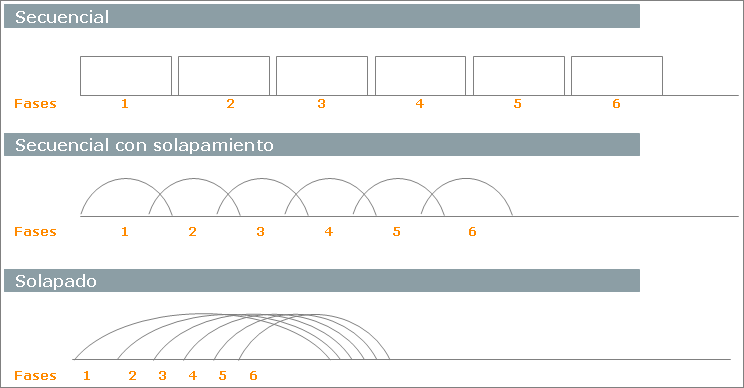
\includegraphics[width=12cm,height=6cm]{figuras/ciclos_desarrollo.png}
\caption{Ciclos de desarrollo.}
\label{fig:ciclos}
\end{figure}

\subsection{Scrum} \label{scrum}
Existen muchas metodologías ágiles disponibles, como el método de desarrollo de sistemas dinámicos (DSDM), la programación extrema (XP), etc. Sin embargo, en este proyecto se hace uso de la metodología Scrum. Actualmente, Scrum es una de las metodologías más populares para la gestión de proyectos. Este modelo fue identificado y definido por Ikujiro Nonaka e Hirotaka Takeuchi a principios de los 80, al analizar cómo desarrollaban los nuevos productos las principales empresas de manufactura tecnológica en esa época. Nonaka y Takeuchi compararon la nueva forma de trabajo en equipo, con el avance en formación de scrum de los jugadores de Rugby, a raíz de lo cual quedó acuñado el término “scrum” para referirse a ella.

Entre las características que describen los entornos de desarrollo típicos en los que se puede aplicar la metodología de desarrollo ágil Scrum, destacan las siguientes:

\begin{itemize}
\item La incertidumbre: Es asumida en el desarrollo del proyecto, en donde se apunta cuál es la visión genérica que se quiere conseguir, o la dirección estratégica que hay que seguir, pero no un plan detallado del producto y su desarrollo (para lo cual se da un margen de libertad).
\item Fases del desarrollo solapadas: Las fases no existen como tal sino que se desarrollan tareas/actividades en función de las necesidades cambiantes durante todo el proyecto. De hecho, en muchas ocasiones no es posible realizar un diseño técnico detallado antes de empezar a desarrollar y ver algunos resultados. En la figura \ref{fig:ciclos}, podemos ver gráficamente en el tercer caso el solapamiento de fases, mientras que en el primer caso el retraso en una fase hace de cuello de botella en el proyecto. El solapamiento diluye el ruido y los problemas entre fases.
\item Control sutil: El equipo trabaja con autonomía en un entorno de ambigüedad, inestabilidad y tensión. La gestión establece puntos de control suficientes para evitar que el ambiente de ambigüedad, inestabilidad y tensión del derive hacia descontrol, pero no ejerce un control rígido que impediría la creatividad y la espontaneidad.
\end{itemize}

En Scrum la gestión no se basa en el seguimiento de un plan, sino en la adaptación continua a las circunstancias de la evolución del proyecto. El desarrollo se inicia desde la visión general de producto, dando detalle  solo a las funcionalidades que, por ser las de mayor prioridad para el negocio, se van a desarrollar en primer lugar, y pueden llevarse a cabo en un periodo de tiempo breve (entre 15 y 60 días). Cada uno de los ciclos de desarrollo es una iteración (sprint) que produce un incremento terminado y operativo del producto. Estas iteraciones son la base del desarrollo ágil, y Scrum gestiona su evolución a través de reuniones breves de seguimiento en las que todo el equipo revisa el trabajo realizado desde la reunión anterior y el previsto hasta la reunión siguiente.

\noindent
\textbf{Roles}
\begin{itemize}
\item \textbf{Propietario del producto (\textit{Product Owner}):} Representa la voz del cliente. Se asegura de que el equipo Scrum trabaje de forma adecuada desde la perspectiva del negocio. Tiene entre sus responsabilidades la financiación, la decisión para efectuar el lanzamiento, etc. También puede escribir historias de usuario, priorizarlas y colocarlas en el \textit{Product Backlog} (descripciones genéricas de todos los requisitos priorizadas de mayor a menor importancia).
\item \textbf{Facilitador (\textit{Scrum Master}):} Responsable de garantizar que se aplica correctamente la metodología. Su trabajo principal es eliminar los obstáculos que impiden que el equipo alcance el objetivo del sprint.
\item \textbf{Equipo desarrollo:} Tiene la responsabilidad de entregar el producto y capacidades para análisis, diseño, desarrollo, pruebas, documentación, etc.
\end{itemize}

\noindent
\textbf{Componentes básicos}
\begin{itemize}
\item \textbf{\textit{Product Backlog}:} Listado general de requisitos que evoluciona durante todo el desarrollo. Todos pueden contribuir y aportar sugerencias y están ordenados por prioridad según el cliente.
\item \textbf{Facilitador (\textit{Sprint Backlog}):} Lista de tareas a realizar en el sprint para generar el incremento. Se asignan los recursos y se estiman las unidades de tiempo para realizar cada tarea.
\item \textbf{Incremento:} Es el resultado de cada sprint listo enseñar al cliente (está terminado y probado) y por tanto en condiciones de ser usado.
\end{itemize}

\noindent
\textbf{Reuniones}
\begin{itemize}
\item \textbf{Planificación del sprint:} Jornada de trabajo previa al inicio de cada sprint en la que se determina cuál es el trabajo y los objetivos que se deben cubrir con esa iteración. Asiste el propietario del producto, el \textit{Scrum Master} y el equipo de trabajo. Esta reunión genera el \textit{Sprint Backlog}.
\item \textbf{Monitorización del sprint:} Reunión diaria donde sólo interviene el equipo y en la que se hace un repaso al avance de cada tarea y al trabajo previsto para la jornada. La duración máxima debe ser de 15 minutos y se recomienda hacerla de pie con los elementos del Sprint Backlog en forma de post-it en una pizarra.
\item \textbf{Revisión del sprint:} Análisis y revisión del incremento generado. Se presenta al cliente el incremento desarrollado (terminado, probado y operando en el entorno del cliente). Se puede obtener feedback para mejorar e incorporar en sucesivos sprints.
\end{itemize}

\begin{figure}[t!]
\centering
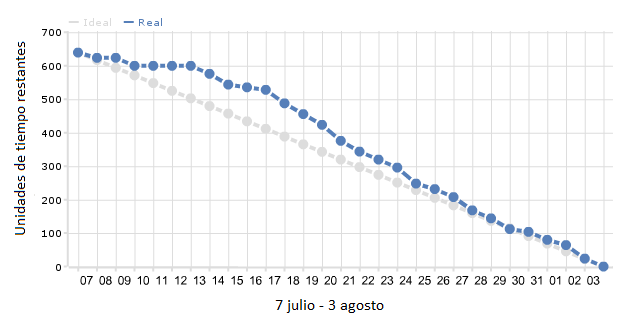
\includegraphics[width=12cm,height=6cm]{figuras/burndown.png}
\caption{Ejemplo gráfico Burn-Down.}
\label{fig:burndown}
\end{figure}

\noindent
\textbf{Gráfico \textit{Burn-Down}}
Herramienta para gestionar y seguir el trabajo de cada sprint, donde se representa gráficamente del avance del sprint. En la figura \ref{fig:burndown} podemos ver este gráfico a modo de ilustración.

\noindent
Las \textbf{modificaciones realizas} sobre la metodología Scrum para realizar este proyecto son dos: 
\begin{itemize}
\item Los roles de \textit{Product Owner} y \textit{Scrum Master} en este proyecto son los mismos, es decir, corresponden a los directores del proyecto, que hacen de voz representativa del cliente y garantizan que se aplique correctamente la metodología. Además, el equipo de desarrollo está representado por una persona.
\item No se realizan las reuniones de monitorización o seguimiento del sprint, ya que en este caso no es necesario realizar un seguimiento tan exhaustivo en el desarrollo y por lo sólo se llevan a cabo cuando existe algún impedimento para continuar con el sprint. Sí se realizan las reuniones de planificación y de revisión del sprint.
\end{itemize}

\noindent
La razón principal de la elección de esta metodología es su flexibilidad a la hora de realizar las diferentes tareas del proyecto, pudiendo seleccionar aquellas tareas que más convienen hacer en un momento dado (las tareas de mayor importancia al principio, para presentar versiones utilizables lo antes posible). Además, en este proyecto existe cierta incertidumbre a la hora de establecer requisitos fijos de antemano, como se puede ver en la sección \ref{riesgos} en el riesgo \textbf{RPD-1}. Así, se desarrollan tareas en función de las necesidades cambiantes durante todo el proyecto y el solapamiento de fases ilustrado en la figura \ref{fig:ciclos} evita que no se tenga que esperar a la finalización de una fase para poder comenzar otra (una de las desventajas de las metodologías pesadas). Otra razón por la que se eligió esta metodología es por la necesidad de ir presentando periódicamente versiones utilizables de la aplicación al cliente (los directores), para que éstos puedan empezar a utilizar la aplicación desde el principio e ir sugiriendo cambios y mejoras a realizar (característica de entornos con incertidumbre). Por ello, las reuniones de planificación y revisión de los sprints (incrementos) son tan importantes en este proyecto.

\section{Gestión de la configuración}
La configuración del software es el conjunto de características funcionales y físicas del software detalladas en la documentación técnica o alcanzadas en un producto. (IEEE610.12-90). La gestión de la configuración, por su parte, es un proceso cuyo propósito es establecer y mantener la integridad de los elementos de trabajo. Para ello, se identifican los elementos y se controlan los cambios de éstos a lo largo de su ciclo de vida, registrando el estado y verificando que estén completos y que sean los correctos.

Para llevar a cabo la gestión de la configuración en este proyecto, se utiliza un sistema de control de versiones mediante la herramienta GitLab que ofrece el CiTIUS y que facilita la gestión de repositorios. Esta herramienta, se basa en GIT, que es un SCV (sistema de control de versiones) multiplataforma y distribuido, donde hay un repositorio central con el cual se puede sincronizar todo el mundo. Se sitúa en una máquina en concreto y es el repositorio que contiene todo el histórico, etiquetas y ramas. La razón de utilizar esta herramienta es su velocidad, su diseño sencillo y la posibilidad de visualizar gráficamente la interacción (gráficas de modificaciones, etc.) con el repositorio.

\noindent
En este proyecto los elementos de configuración implican tanto los archivos de desarrollo como los archivos de documentación:
\begin{itemize}
\item Módulo de Python de los tests estadísticos (paramétricos y no paramétricos).
\item API REST.
\item Archivos de la web: archivos HTML, CSS, JavaScript, imágenes, etc.
\item Memoria.
\item Documentación del módulo de Python de los tests estadísticos.
\end{itemize}

\noindent
El proceso de gestión de configuración es el siguiente:
\begin{enumerate}
\item Se dispone de una rama principal denominada \textit{master} que hace la labor de \textbf{línea base} (donde se encuentran los archivos de los sprints finalizados, es decir, los archivos con los cambios del último sprint).
\item Para mantener organizada y de forma accesible la información, cada sprint se realiza en una rama de desarrollo separada de la rama \textit{master}. Cuando se finaliza el sprint se fusiona en la rama principal.

- La nomenclatura de las ramas será la siguiente: ``sprintX", donde X representa el número de sprints actual.

- En la rama de desarrollo del sprint se van realizando los cambios a los archivos, indicando con una breve descripción los cambios que se hacen.
\item Al finalizar cada sprint, también se crea una etiqueta o \textit{tag} de la rama de desarrollo para tener disponibles todas las versiones de la aplicación (todos los sprints) en un archivo comprimido.

- La nomenclatura de las etiquetas será la siguiente: ``v0.X", donde X representa el número de sprints actual.
\end{enumerate}

\section{Planificación temporal}

\section{Estimación de costes}
\cleardoublepage
\chapter{Arquitectura y herramientas} \label{arquitecturayh}
El proceso de diseñar es definido por el IEEE como el esfuerzo para definir la arquitectura, componentes, interfaces y otras características de un sistema o componente. También se podría definir como la etapa del ciclo de vida del software en la cual se produce una descripción de la estructura interna del software que sirve de base para su construcción. El estándar ISO 12207 identifica un diseño a alto nivel o arquitectónico y un diseño detallado. El primero describe la estructura y organización, es decir, los subsistemas o componentes y sus relaciones. El segundo, describe cada componente y su comportamiento específico, para proceder a su construcción.

Después de tener una idea formada de los objetivos y requisitos del presente proyecto, en este capítulo nos centraremos en el diseño de alto nivel o la arquitectura, donde además de utilizar representaciones gráficas a alto nivel del sistema se detallarán las tecnologías y elementos arquitectónicos básicos del mismo, así como las herramientas utilizadas para llevar a cabo el proyecto.

\section{Arquitectura del sistema} \label{arquitectura}
Analizando los requisitos y los objetivos del proyecto se identifican tres partes críticas en el sistema: la interfaz gráfica de usuario (interfaz web), el API de los servicios web de los test estadísticos y el módulo STAC (\textit{Statistical Tests for Algorithm Comparison}), donde están incluidos los propios test estadísticos (tanto los test paramétricos como los test no paramétricos). En la figura \ref{fig:arquitectura} podemos ver la arquitectura de la plataforma web:

\begin{figure}[H]
\centering
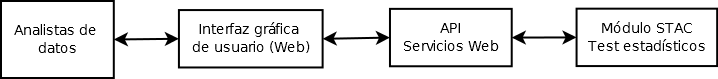
\includegraphics[width=15cm]{figuras/arquitectura.png}
\caption{Arquitectura de la plataforma web.}
\label{fig:arquitectura}
\end{figure}

Como podemos ver, los usuarios están representados como analistas de datos, y hacen uso de la interfaz gráfica de usuario (interfaz web), donde pueden realizar tareas tales como subir sus resultados y visualizarlos para posteriormente poder aplicar sobre ellos alguno de los test disponibles en el sistema. Esta interfaz representa la cara visible hacia el usuario, y por tanto será lo más usable posible para facilitar la tarea de validación.

La interfaz gráfica a su vez se comunica con el API de los servicios web, que son los encargados de ejecutar los test estadísticos con los parámetros u opciones elegidas por el analista en la interfaz (nivel de significancia, etc.), y devolver los datos obtenidos por el test a la interfaz para que ésta represente los datos de la forma más cómoda posible.

Por último, la parte más importante de la plataforma está representada por el módulo STAC, compuesto tanto por test paramétricos como no paramétricos. Aquí el usuario dispone de varios test, entre los que se encuentran por ejemplo aquellos que verifican si se cumplen las condiciones de homocedasticidad o normalidad para determinar si se pueden aplicar con seguridad (fiabilidad) test paramétricos.

Con el objetivo de desacoplar los datos y la lógica de negocio (modelo) de la interfaz de usuario (vista) y el módulo encargado de gestionar los eventos (controlador), se ha aplicado el patrón MVC (Modelo-vista-controlador) para construir la plataforma web. El concepto de patrón de diseño se explicará en más profundidad en secciones posteriores. En la figura \ref{fig:mvc} se muestra una representación gráfica de esta arquitectura, que ha sido en la que se ha basado este proyecto y en la que se distinguen las siguientes partes:

\begin{figure}[H]
\centering
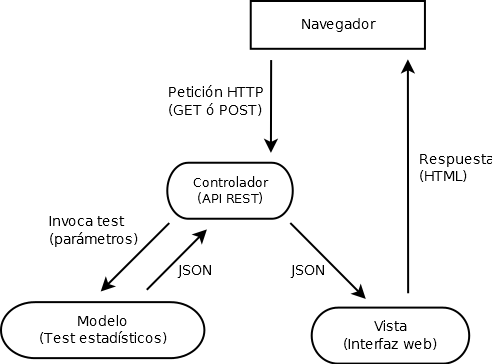
\includegraphics[width=9cm]{figuras/mvc.png}
\caption{Patrón MVC.}
\label{fig:mvc}
\end{figure}

\begin{itemize}
\item El controlador se encarga de recibir las peticiones HTTP (GET o POST) del navegador y decide qué test estadístico quiere invocar (para lo cual realizará una llamada con ciertos parámetros). La subida y visualización de ficheros de datos son tratados por el propio controlador. Éste una vez obtenga los datos se los devolverá a la vista (en formato JSON). En este proyecto el controlador está representado por el API de servicios web REST.
\item Las vistas reciben los datos del modelo a través del controlador y se los muestran a los usuarios (en formato HTML), en ellas únicamente se realizan operaciones simples. Representa la interfaz gráfica de usuario (Web).
\item El modelo es el responsable de realizar una gran parte de las funcionalidades del sistema, ya que en él se lleva a cabo la realización de las distintas pruebas de hipótesis. Esta parte representaría al módulo STAC, en donde se localizan los test paramétricos y no paramétricos.
\end{itemize}

Las tecnologías mencionadas (HTTP, REST, JSON) se detallan en secciones posteriores dentro del presente capítulo.

\section{Herramientas de diseño}
En este proyecto se utiliza la programación modular como paradigma de programación. La programación modular consiste en dividir un programa en módulos o subprogramas con el fin de hacerlo más legible y manejable. Un módulo es cada una de las partes de un programa que resuelve uno de los subproblemas en que se divide el problema complejo original. Cada uno de estos módulos tiene una tarea bien definida y algunos necesitan de otros para poder operar. La razón de realizarlo de esta forma y no orientado a objetos es debido a que los test estadísticos implementados son funciones en sí, los cuales reciben una serie de parámetros y devuelven unos resultados. Para el caso de la API REST, el framework elegido que se verá en secciones posteriores hace también que los servicios web tengan una representación en forma de función, con lo que sería añadir una complejidad extra al proyecto innecesaria.

Para poder modelar el software de un modo formal se utilizará UML (\textit{Unified Modeling Language}). UML es un lenguaje gráfico para visualizar, especificar y documentar cada una de las partes que comprende el desarrollo de software. Permite especificar diferentes ámbitos del sistema desde la lógica de negocio hasta la estructura hardware, sin ligarse a ningún lenguaje de desarrollo en particular. Para ello, hace uso de modelos que representan el sistema desde un punto de vista específico.

UML proporciona 13 tipos de diagramas, que se dividen en tres categorías: estructura, comportamiento e interacción. Pese a que UML está por lo general ligado a la programación orientada a objetos, en este proyecto se utilizará para realizar un diagrama de la categoría de interacción, que servirá para definir acciones que se pueden realizar en la plataforma:

\noindent
\begin{itemize}
\item \textbf{Diagramas de secuencia:} indican los componentes que forman parte del sistema y las llamadas que se hacen en cada uno de ellos para realizar una tarea determinada. Los mensajes o llamadas intercambiados están ordenados temporalmente (en secuencia).
\end{itemize}

\subsection{Herramientas}
Para poder realizar los diagramas UML y el prototipo de la interfaz gráfica del usuario, se han utilizado las siguientes herramientas:

\begin{itemize}
\item \textbf{StarUML:} herramienta que soporta la mayoría de los tipos de diagramas especificados en UML 2.0 y que servirá para realizar los diagramas en este proyecto.
\item \textbf{Lumzy:} herramienta de creación de prototipos para sitios web y aplicaciones.
\end{itemize}

\subsection{Patrones de diseño}
Un patrón es una solución a un problema en un contexto particular. Es recurrente (lo que hace la solución relevante a otras situaciones), enseña (permite entender cómo adaptarlo a la variante particular del problema donde se quiere aplicar) y tiene un nombre para referirse al patrón. Los patrones facilitan la reutilización de diseños y arquitecturas software que han tenido éxito. Existen tres categorías de patrones de diseño:
\begin{itemize}
\item \textbf{Patrones de creación:} tratan de la inicialización y configuración de clases y objetos.
\item \textbf{Patrones estructurales:} tratan de desacoplar interfaz e implementación de clases y objetos.
\item \textbf{Patrones de comportamiento:} tratan de las interacciones dinámicas entre sociedades de clases y objetos.
\end{itemize}

Debido a que los patrones de diseño están fuertemente ligados al paradigma orientado a objetos (clases y objetos), en este proyecto se utilizan solamente dos patrones:
\begin{itemize}
\item \textbf{El patrón MVC:} visto en la sección \ref{arquitectura}, encaja dentro de los denominados patrones estructurales, y sirve para desacoplar interfaz e implementación
\item \textbf{El patrón \textit{Singleton} (Fig. \ref{fig:singleton}):} para la implementación de la historia de usuario \textbf{HU-5} vista en la sección \ref{hu_desarrollador}. Este es el único punto del proyecto donde se utiliza programación orientada a objetos. La razón de utilizar una clase para implementar la \textbf{HU-5} en este caso se facilita la programación de esta característica del proyecto.
\end{itemize}

\noindent
\textbf{Patrón Singleton}

Este patrón está diseñado para restringir la creación de objetos pertenecientes a una clase o el valor de un tipo a un único objeto. Su intención consiste en garantizar que una clase sólo tenga una instancia y proporcionar un punto de acceso global a ella (Fig. \ref{fig:singleton}). El patrón \textit{singleton} se implementa creando en nuestra clase un método que crea una instancia del objeto sólo si todavía no existe alguna. Para asegurar que la clase no puede ser instanciada nuevamente se regula el alcance del constructor (con atributos como protegido o privado).

\begin{figure}[H]
\centering
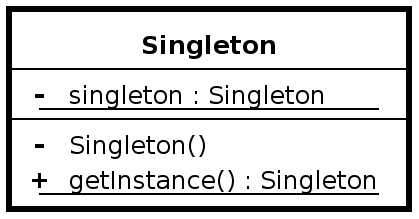
\includegraphics[width=6cm,height=3cm]{figuras/singleton.png}
\caption{Patrón \textit{Singleton}.}
\label{fig:singleton}
\end{figure}

\section{Herramientas de desarrollo}

\subsection{Análisis de librerías de test estadísticos en Python} \label{libreriastest}

\subsubsection{\textbf{Librería SciPy - \textit{Scientific Computing Tools for Python}}}
SciPy \cite{scipy} cuenta con una colección denominada \textit{The SciPy Stack}, que consta de un conjunto de paquetes principales de software de código abierto para la computación científica en Python, donde la comunidad puede utilizar y desarrollar esta colección. Entre los paquetes básicos de esta colección se encuentran:
\begin{itemize}
\item \textbf{NumPy:} paquete fundamental para computación numérica, donde se puede encontrar álgebra lineal, operaciones estadísticas básicas (como la media, la varianza, ...), aleatoriedad, etc. 
\item \textbf{Librería SciPy:} una colección de algoritmos numéricos y herramientas específicas de dominio, incluyendo el procesamiento de señales, la optimización, estadística, etc.
\end{itemize}
SciPy y NumPy tienen versiones de documentación en formato HTML y PDF \cite{scipy-doc}, que cubren casi toda la funcionalidad disponible.
La librería SciPy es uno de los paquetes principales que componen \textit{The SciPy Stack}. Proporciona muchas rutinas numéricas fáciles de usar y eficientes, como las rutinas de integración numérica y optimización. SciPy está organizada en subpaquetes o módulos que cubren diferentes dominios de computación científica. Para este proyecto, el subpaquete que nos interesa es \textit{\textbf{stats}}, que consta de distribuciones y funciones estadísticas.

El subpaquete \textit{stats} contiene un gran número de distribuciones de probabilidad (tanto continuas como discretas). Las continuas (como la distribución $\chi^2$ ó $\mathcal{T}$ vistas en la sección \ref{estadistico}) son las que nos interesan. Estas distribuciones continuas definidas como clases constan de métodos comunes, como son la función de densidad de probabilidad o la función de distribución acumulada para una distribución determinada, de las que ya hemos hablado en la figura \ref{fig:comparativa_pdf_cdf}. Estas funciones sirven de utilidad para realizar los test estadísticos y obtener valores necesarios. Así mismo, este módulo proporciona también una biblioteca de test estadísticos. Entre estos test están aquellos para hallar las condiciones paramétricas de normalidad (Shapiro-Wilk, D’Agostino–Pearson y Kolmogorov–Smirnov), y homocedasticidad (Levene), así como la prueba $\mathcal{T}$ de Student (vistos en la sección \ref{parametricos} del capítulo \ref{contraste}). 

Un módulo de la librería SciPy se define como un subpaquete Python del paquete SciPy: scipy/subpaquete. Este subpaquete contiene los archivos de Python con el código de las diferentes funcionalidades, así como aquellos archivos de inicialización e importación que sirven para facilitar su uso.

Por tanto, para este proyecto nos serviremos de los test de las condiciones paramétricas, así como de la prueba $\mathcal{T}$ de Student incluidos en esta librería, ya que forman parte de los objetivos del proyecto. Sin embargo, esta librería no cubre todas las necesidades de test detalladas en los objetivos para el proyecto.
 
\subsubsection{\textbf{Librería nonparametric.py}} \label{nonparametric}
Este módulo, creado por Ismael Rodríguez, contiene algunos de los test marcados como objetivos en este proyecto: el test de Wilcoxon, el test de Friedman, el test de Iman-Davenport, el test de Bonferroni-Dunn, el test de Holm y el test Hochberg. Sin embargo, no se ha probado su correcto funcionamiento y por tanto algunos de ellos necesitarán ser rediseñados e implementados de nuevo. Para ello será necesario:

\begin{itemize}
\item Probar que funcionan correctamente mediante la realización de test unitarios y corregir los fallos encontrados.
\item Comprobar que devuelven los datos necesarios: rankings, estadísticos, $\textit{p-valor}$ (en caso de los test de ranking); y los parámetros usados para cada comparación, $\textit{p-valor}es$ ajustados (en el caso de los test de comparación).
\item Hacer que reciban y devuelvan los datos de la misma manera. 
\end{itemize}

Este módulo tiene dependencias con la librería SciPy (con el módulo \textit{stats}), así como con el paquete NumPy. Como se ha dicho anteriormente, la funcionalidad de SciPy sirve a este proyecto para poder hallar parámetros básicos que serán necesarios para obtener todos los datos necesarios en los test.

Dado que será necesario corregir y volver a implementar muchas de las funcionalidades presentes en este módulo, y debido a que muchas otras funcionalidades aún quedan por implementar, este módulo tampoco cumple con las expectativas del proyecto. La extensión y corrección de este módulo permitirá la obtención de un módulo acorde a los objetivos del proyecto con todos los test disponibles. 

\subsection{Análisis de librerías para servicios REST en Python} \label{bottle}

\subsubsection{\textbf{Servicios REST}}
Los test estadísticos, así como la subida y consulta de ficheros serán accesibles vía web mediante servicios web en Python y basados en REST. La Transferencia de Estado Representacional (\textit{Representational State Transfer}) o REST es una técnica de arquitectura software para sistemas hipermedia distribuidos como la World Wide Web. El término se originó en el año 2000, en una tesis doctoral sobre la web escrita por Roy Fielding, uno de los principales autores de la especificación del protocolo HTTP y ha pasado a ser ampliamente utilizado por la comunidad de desarrollo. Aunque REST no es un estándar, está basado en los estándares: HTTP, URL, representación de los recursos (XML, HTML, GIF, JPEG, JSON ...), y tipos MIME (text/xml, text/html, application/json, ...)

Por ejemplo, en la figura \ref{fig:rest} se puede ver como ejemplo una petición para consultar el contenido de un archivo. Para ello, la respuesta indica en la cabecera con ``Content-Type: application/json", el tipo de dato a devolver, por lo que el cliente sabe que el contenido de la respuesta es una cadena en formato JSON, y puede procesarla como prefiera. Los servicios web REST están basados en los siguientes principios:

\begin{itemize}
\item \textbf{Utilización de métodos HTTP:} por tanto, los métodos a utilizar para la comunicación con los servicios web de los test podrán ser los comunes de HTTP: GET, POST, PUT, DELETE.
\item \textbf{Servicios sin estado:} las peticiones a los servicios web de los test incluirán todos los datos necesarios (petición completa e independiente) para que el servidor no tenga que mantener ningún estado para procesar la petición. En otras palabras, el servidor no puede almacenar información proporcionada por el cliente en una solicitud y usarlo en otra solicitud.
\item \textbf{Exposición de URIs (identificador recursos uniforme) con forma de directorios:} por ejemplo, se podrían hacer URIs del estilo: http://localhost/api/nombre\_test/...
\end{itemize}

\begin{figure}[H]
\centering
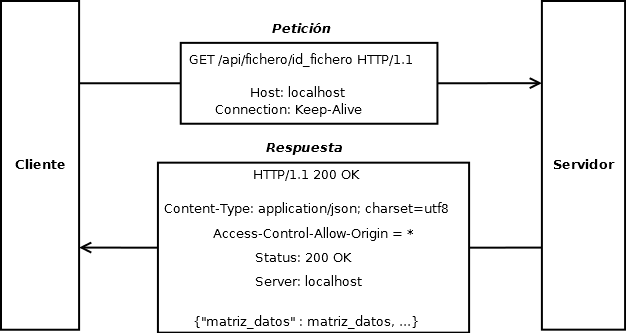
\includegraphics[width=12cm,height=6cm]{figuras/rest.png}
\caption{Servicios web REST.}
\label{fig:rest}
\end{figure}

Cabe destacar que para el presente proyecto se utilizarán los métodos HTTP GET y POST, el primero para obtener información de un recurso (esto es, obtener los resultados de los test, así como el contenido del fichero) y el segundo para crear un nuevo recurso (para la creación de un nuevo fichero). Así mismo, los recursos estarán representados por el tipo MIME ``application/json". La figura \ref{fig:rest} muestra estas características.

\subsubsection{\textbf{Librería Bottle}}
Para desarrollar los servicios web que diesen acceso a los test estadísticos, así como a la gestión del fichero, en el anteproyecto se había barajado la utilización de alguno de los siguientes frameworks: Flask, Web.py y Bottle. El framework elegido finalmente fue Bottle \cite{bottle}. Este framework web es conocido más bien como un micro framework, y las principales razones que propiciaron su elección frente a las demás es que se trata de un framework rápido, sencillo y ligero para Python. Se distribuye como un módulo y esta formado por un único archivo y no tiene dependencias distintas de la biblioteca estándar de Python. Además, dispone de las siguientes características:
\begin{itemize}
\item \textbf{Enrutamiento:} mapeo de solicitudes de llamadas a función con soporte para URLs limpias y dinámicas.
\item \textbf{Plantillas:} motor de plantillas integrado.
\item \textbf{Utilidades:} la facilidad de acceso a datos de formulario, subida de ficheros, cookies, cabeceras y otros metadatos relacionados con HTTP.
\item \textbf{Servidor:} servidor HTTP propio para desarrollo integrado y soporte para cualquier servidor HTTP compatible con la especificación WSGI (interfaz entre servidores web y aplicaciones web o frameworks para el lenguaje Python).
\end{itemize}

Bottle permite la implementación de servicios web accesibles mediante una o más URIs. El decorador \textit{route()} asigna una URI a un trozo de código (el propio servicio) en lo que se denomina ruta. El decorador decora a lo que realmente referencia, que es un trozo de código. Cada vez que el navegador llama a una URL especificada con \textit{route()} la función o servicio asociado es llamado y el valor de retorno se envía al navegador. A un mismo servicio se pueden unir tantas URIs como se desean. El siguiente código muestra cómo de una forma sencilla se puede implementar un servicio REST:

\begin{lstlisting}
@route('/fichero/<id_fichero>', method='GET')
def consultar_fichero(id_fichero):
    response.headers['Access-Control-Allow-Origin'] = '*'
    response.content_type = "application/json"
    ...
    return datos
\end{lstlisting}

Como se puede ver en ejemplo, por medio de \textit{@route} se indica la URL. El método utilizado en este caso es GET y la respuesta será dada en formato JSON. Con \textit{id\_fichero}, se indica que se va a pasar el identificador del fichero como parte de la URL.

\subsection{Análisis de frameworks para desarrollo web}

\subsubsection{\textbf{Twitter Bootstrap}}
El framework para el desarrollo de la interfaz web utilizado en la plataforma es Twitter Bootstrap \cite{bootstrap}. Bootstrap fue desarrollado por Mark Otto y Jacbod Thornton de Twitter, como solución interna para solucionar las inconsistencias en el desarrollo dentro del equipo de ingeniería de Twitter, ya que hasta ese momento no había establecida ninguna convención sobre las formas en las que los ingenieros desarrollaban la plataforma. En agosto del 2011, Twitter liberó a Bootstrap como código abierto. En febrero del 2012, se convirtió en el proyecto de desarrollo más popular de GitHub \cite{github} y es utilizado por organizaciones como la NASA.

Se trata de un framework o conjunto de herramientas de software libre para diseño de sitios y aplicaciones web (\textit{Front-end} o interfaz). Contiene plantillas de diseño con tipografía, formularios, botones, cuadros, menús de navegación y otros elementos de diseño basado en HTML5 y CSS3, así como, extensiones de JavaScript opcionales adicionales. Una de sus principales características es que utiliza LESS, que es una ampliación de las hojas de estilo CSS, pero a diferencia de estás, funciona como un lenguaje de programación, permitiendo el uso de variables, funciones, operaciones aritméticas, entre otras, para acelerar y enriquecer los estilos en un sitio web.

\begin{figure}[H]
\centering
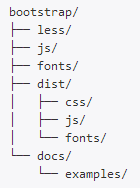
\includegraphics{figuras/bootstrap.png}
\caption{Organización Twitter Bootstrap.}
\label{fig:booststrap}
\end{figure}

La figura \ref{fig:booststrap} muestra la organización de directorios de Bootstrap. Los directorios less/, js/ y fonts/ contienen el código fuente utilizado para generar los archivos CSS, JavaScript y las fuentes. El directorio dist/ contiene los mismos archivos que se han mostrado en la sección anterior para la versión compilada de Bootstrap. El directorio docs/ incluye el código fuente de la documentación de Bootstrap y el directorio examples/, que contiene varios ejemplos de muestra. El resto de archivos incluidos proporcionan información de licencia y desarrollo.

Las razones de la utilización de este framework se basan en la sencillez y en la amplia documentación existente. Sin embargo, la razón principal es la capacidad para diseño \textit{responsive} o fluido (\textit{responsive design}). Mediante el diseño responsivo, se consigue que la web se adapte según según la resolución del dispositivo o ventana del navegador. Esto es necesario para poder desarrollar de un modo fácil y adecuado la historia de usuario \textbf{HU-5} vista en la sección \ref{hu_cliente} del capítulo \ref{analisisreq}. Para este propósito, Bootstrap cuenta con un diseño de páginas basado en rejillas, que están formadas por de filas y columnas donde se colocan los contenidos. Las rejillas crecen hasta 12 columnas a medida que crece el tamaño de la pantalla del dispositivo.

\subsection{Otras herramientas}
\subsubsection{\textbf{Desarrollo}}
Con el objetivo de disminuir los costes del proyecto, y teniendo en cuenta el uso de herramientas que requieran el menor tiempo de aprendizaje, el entorno de trabajo seleccionado para el desarrollo del proyecto fue el siguiente:
\begin{itemize}
\item \textbf{Sistema operativo:} Ubuntu 12.04, basado GNU/Linux.
\item \textbf{IDE de programación:} Spyder 2, entorno multiplataforma de código abierto para la programación científica en el lenguaje Python. La razón de su utilización es que Spyder integra NumPy y SciPy, entre otras librerías.
\end{itemize}
\subsubsection{\textbf{Documentación}}
Para el desarrollo de la documentación se han utilizado las siguientes herramientas:
\begin{itemize}
\item \textbf{Sphinx 1.2.2:} Sphinx se trata de una herramienta de código abierto para generación de documentación de código Python. Es utilizada para documentar el módulo de Python STAC perteneciente a los test estadísticos. La razón de su utilización es que permite la generación de documentación en formato HTML para poder acceder a ella desde el navegador. Además, permite la escritura de fórmulas mediante notación \LaTeX, lo cual es importante en este proyecto.
\item \textbf{TeXstudio 2.8.2:} IDE de código abierto de \LaTeX \space que proporciona un soporte moderno de escritura, corrección ortográfica interactiva, plegado de código y resaltado de sintaxis. Es utilizado para la realización de la documentación.
\item \textbf{ProjectLibre 1.5.9:} herramienta multiplataforma de código abierto utilizada para la elaboración de diagramas de Gantt.
\item \textbf{Dia 0.97.2:} herramienta multiplataforma de código abierto utilizada para la elaboración de diagramas en general. Es utilizada en este proyecto para elaborar el EDT, así como diagramas genéricos de arquitectura, etc.
\end{itemize}

\subsubsection{\textbf{Tecnologías}} \label{tecnologias}
A parte de las tecnologías anteriormente mencionadas, el desarrollo del proyecto también está marcado por la utilización de las siguientes otras:

\begin{itemize}
\item \textbf{HTML:} \textit{HyperText Markup Language}, hace referencia al lenguaje de marcado para la elaboración de páginas web. Es un estándar que, en sus diferentes versiones, define una estructura básica y un código para la definición de contenido de una página web, como texto, imágenes, etc.
\item \textbf{JavaScript:} es un lenguaje de programación interpretado. Se utiliza en páginas web HTML para realizar
operaciones en el marco de la aplicación cliente, sin acceso a funciones del servidor.
\item \textbf{CSS:} \textit{Cascading style sheets} u hojas de estilo en cascada es un lenguaje usado para definir la presentación de un documento estructurado escrito en HTML.
\item \textbf{Apache y el módulo WSGI:} a pesar de que el framework Bottle dispone de su propio servidor HTTP para desarrollo integrado, y aprovechando que soporta cualquier servidor HTTP compatible con la especificación WSGI, en este proyecto se optó por la utilización del servidor web Apache. La principal razón de realizarlo de este modo es que el tiempo de respuesta del servidor de Bottle era de 5 segundos cuando se accedía desde otra red, mientras que utilizando Apache se llega a bajar a 2-3 milisegundos. Además, con esto se consigue hacer disponible la API REST por el puerto 80.
\subitem \textbf{- Apache} es un servidor web HTTP de código abierto, que implementa el protocolo HTTP/1.12. Desde 1996, Apache es el servidor HTTP más usado. Alcanzó su máxima cuota de mercado en 2005 siendo el servidor empleado en el 70\% de los sitios web en Internet.
\subitem \textbf{- WSGI} es una interfaz o especificación entre servidores web y aplicaciones web o frameworks para el lenguaje Python. El módulo WSGI de Apache implementa la interfaz WSGI, lo cual permite servir las aplicaciones Python (nuestro caso el API REST).
\item \textbf{AJAX:} \textit{Asynchronous JavaScript} + XML, está formada varias por tecnologías que permiten realizar peticiones HTTP y modificaciones en las páginas de forma asíncrona sin necesidad de recargar la página. Entre los beneficios del uso de AJAX destaca la reducción del tráfico con el servidor. Es utilizada en este proyecto para poder llamar a los servicios REST y gestionar los datos devueltos por éstos (interacción con las páginas HTML).
\item \textbf{JSON:} \textit{JavaScript Object Notation}, es un formato ligero para el intercambio de datos. Es utilizado por AJAX y los servicios REST. La razón de la utilización de este formato es que puede ser interpretado por cualquier lenguaje (incluido Python). En la figura \ref{fig:rest} podemos ver un ejemplo de formato JSON en la respuesta a la petición.
\end{itemize}

\subsubsection{\textbf{Librerías}}
En la siguiente tabla se muestran las distintas librerías de JavaScript utilizadas en el desarrollo del proyecto:

\begin{table}[H]
	\centering
	\begin{tabular}{|l|c|c|}
		\hline
		\textbf{Librería} & \textbf{Versión} & \textbf{Página Oficial} \\ \hline
		jQuery & 1.11.0 & http://jquery.com/ \\ \hline
		MathJax & 2.4 & http://www.mathjax.org/ \\ \hline
	\end{tabular}
\end{table}

\begin{itemize}
\item \textbf{jQuery:} es una biblioteca de JavaScript que permite simplificar la manera de interactuar con los documentos HTML, manipular el árbol DOM, manejar eventos, desarrollar animaciones y agregar interacción con la técnica AJAX a páginas web. Es utilizada en este proyecto para trabajar junto con el framework Bootstrap y para realizar las llamadas AJAX a los servicios web.
\item \textbf{MathJax:} es un motor de visualización de código libre de JavaScript que permite visualizar fórmulas matemáticas en navegadores web, utilizando diferentes lenguajes de marcado (entre ellos \LaTeX). MathJax tiene licencia libre y funciona en todos los navegadores modernos. La razón de su utilización en el proyecto es que en alguna ocasión se necesita escribir fórmulas en documentos HTML, y esta librería constituye una manera fácil de llevar a cabo esta tarea.
\end{itemize}
\cleardoublepage
\chapter{Diseño e implementación}
Una vez diseñada la arquitectura de la plataforma, es necesario detallar el proceso de creación de cada una de las unidades de las que consta la aplicación. Para ello, en primer lugar, se explicará como está organizado y desarrollado el módulo de Python de los test estadísticos. En segundo lugar, se detallará el diseño de la API REST desde el punto de vista de las URIs que conforman cada servicio web. Por último, se detallará la capa superior de la arquitectura, explicando cómo será la interfaz gráfica mediante prototipado y analizando su nivel de usabilidad mediante los principios heurísticos de Nielsen. Así mismo, se hará uso de UML para especificar los diagramas de secuencia de las funcionalidades más relevantes del sistema.

\section{Módulo Python test estadísticos} \label{dis_py}
El módulo de Python de los test estadísticos o módulo STAC (Statistical Tests for Algorithm Comparison) está formado por los siguientes archivos:
\begin{itemize}
\item \textbf{tests\_parametricos.py:} contiene el test paramétrico ANOVA y el test POST-HOC de Bonferroni para el test de ANOVA.
\item \textbf{tests\_no\_parametricos.py:} contiene todos los test no paramétricos (Wilcoxon, Friedman, etc.) indicados en los objetivos del proyecto, excepto aquellos que ya se encuentran en la librería SciPy, tal y como se indicó en la sección \ref{libreriastest}.
\item \textbf{\_\_init\_\_.py:} para que los archivos de test puedan ser importados todos a la vez, es posible empaquetarlos juntos. En este fichero se indica qué se importará al importar el módulo.
\end{itemize}
Este módulo, como se había comentado en la sección \ref{nonparametric} del capítulo \ref{arquitecturayh}, tiene dependencias con la librería SciPy (con el módulo \textit{stats}), así como con el paquete NumPy. La funcionalidad de SciPy sirve a este proyecto para poder hallar parámetros básicos que serán necesarios para obtener todos los datos necesarios en los test.

El diseño del los test estadísticos está determinado por los argumentos de entrada y valores de salida cada test.

\subsection{Test paramétricos}

\noindent
\textbf{Prototipo de la función del test ANOVA:}

\texttt{anova\_test(matriz\_datos, alpha=0.05)}

\begin{itemize}
\item \textbf{``matriz\_datos":} lista de listas de conjuntos de datos. Cada conjunto de datos representa los resultados obtenidos por los algoritmos al ser aplicados sobre un problema concreto.
\item \textbf{``alpha":} nivel de significación o error tipo I (probabilidad de rechazar la hipótesis nula siendo cierta).
\end{itemize}

\noindent
\textbf{Datos devueltos:}

Diccionario que contiene los siguientes datos:

\begin{itemize}
\item \textbf{``resultado":} \textit{true} ó \textit{false}, que indica que el contraste es estadísticamente significativo o estadísticamente no significativo, dependiendo de si el p\_valor es menor que el nivel de significación.
\item \textbf{``p\_valor":} probabilidad de obtener un valor al menos tan extremo como el estadístico hallado suponiendo la hipótesis nula cierta.
\item \textbf{``estadístico":} valor del estadístico en cuestión.
\item \textbf{``variaciones":} lista con las variaciones o sumas de cuadrados total, entre tratamientos y variación del error (SCT, SCTR, SCE).
\item \textbf{``grados\_libertad":} lista con los grados de libertad totales, entre tratamientos y del error (GLT, GLTR, GLE).
\item \textbf{``cuadrados\_medios":} lista con los cuadrados medios (suma cuadrados / grados libertad) total, entre tratamientos y variación del error (SCT, SCTR, SCE).
\item \textbf{``medias\_algoritmos":} lista con las medias de los datos de cada tratamiento o algoritmo.
\item \textbf{``media\_general":} media de la lista de medias de los algoritmos.
\end{itemize}

\noindent
\textbf{Prototipo de la función del test POST-HOC Bonferroni:}

\texttt{bonferroni\_test(nombres\_algoritmos, medias\_algoritmos, cuadrado\_medio\_error, N, alpha=0.05)}

\begin{itemize}
\item \textbf{``nombres\_algoritmos":} lista de los nombres de los algoritmos.
\item \textbf{``medias\_algoritmos":} lista con las medias de los datos de cada tratamiento o algoritmo.
\item \textbf{``cuadrado\_medio\_error":} valor del cuadrado medio del error (suma cuadrados error / grados libertad error).
\item \textbf{``N":} número de conjuntos de datos.
\item \textbf{``alpha":} nivel de significación o error tipo I (probabilidad de rechazar la hipótesis nula siendo cierta).
\end{itemize}

\noindent
\textbf{Datos devueltos:}

Diccionario que contiene los siguientes datos:

\begin{itemize}
\item \textbf{``resultado":} lista de valores \textit{true} ó \textit{false}, que indica si cada uno de los contrastes es o no estadísticamente significativo, dependiendo de si cada uno de los p\_valores es menor que el nivel de significación.
\item \textbf{``p\_valores":} lista de probabilidades de obtener un valor al menos tan extremo como cada uno de los estadísticos hallados suponiendo la hipótesis nula cierta.
\item \textbf{``valores\_t":} lista de valores o estadísticos para cada comparación.
\item \textbf{``p\_valores ajustados":} lista de los p\_valores de las comparaciones ajustados a toda la familia de comparaciones.
\item \textbf{``alpha":} nivel de significación (modificado según el valor de m).
\item \textbf{``comparaciones":} lista donde cada elemento es un texto que contiene los nombres de los dos algoritmos involucrados en la comparación tal como “algoritmoA vs algoritmoB”. Se ordena según del p\_valor de la comparación.
\end{itemize}

\subsection{Test no paramétricos}

\noindent
\textbf{Prototipos de la función del test no paramétricos de Wilcoxon:}

\texttt{wilcoxon\_test(matriz\_datos, alpha=0.05)}

\begin{itemize}
\item \textbf{``matriz\_datos":} lista de listas de conjuntos de datos. Cada conjunto de datos representa los resultados obtenidos por los algoritmos al ser aplicados sobre un problema concreto.
\item \textbf{``alpha":} nivel de significación o error tipo I (probabilidad de rechazar la hipótesis nula siendo cierta).
\end{itemize}

\noindent
\textbf{Datos devueltos:}

Diccionario que contiene los siguientes datos:

\begin{itemize}
\item \textbf{``resultado":} \textit{true} ó \textit{false}, que indica que el contraste es estadísticamente significativo o estadísticamente no significativo, dependiendo de si el p\_valor es menor que el nivel de significación.
\item \textbf{``estadistico":} valor del estadístico en cuestión.
\item \textbf{``suma rangos pos":} suma de los rangos de las diferencias mayores que 0.
\item \textbf{``suma rangos neg":} suma de los rangos de las diferencias menores que 0.
\item \textbf{Si $N \leq 25$ (tamaño muestral):}
\subitem \textbf{- ``punto critico"} límite inferior del intervalo de aceptación. El contraste será estadísticamente significativo si: estadístico $\leq$ límite inferior correspondiente.
\item \textbf{Si $N > 25$:}
\subitem \textbf{- ``p\_valor":} probabilidad de obtener un valor al menos tan extremo como el estadístico hallado suponiendo la hipótesis nula cierta.
\end{itemize}

\noindent
\textbf{Prototipos de las funciones test no paramétricos de ranking:}

\texttt{friedman\_test(nombres\_algoritmos, matriz\_datos, alpha=0.05, tipo=0)}

\texttt{iman\_davenport\_test(nombres\_algoritmos, matriz\_datos, alpha=0.05, tipo=0)}

\texttt{friedman\_rangos\_alineados\_test(nombres\_algoritmos, matriz\_datos, alpha=0.05, tipo=0)}

\texttt{quade\_test(nombres\_algoritmos, matriz\_datos, alpha=0.05, tipo=0)}

\begin{itemize}
\item \textbf{``nombres\_algoritmos":} lista que contiene los nombres de los algoritmos y que será empleada para devolver el ranking de nombres de los algoritmos.
\item \textbf{``matriz\_datos":} lista de listas de conjuntos de datos. Cada conjunto de datos representa los resultados obtenidos por los algoritmos al ser aplicados sobre un problema concreto.
\item \textbf{``alpha":} nivel de significación o error tipo I (probabilidad de rechazar la hipótesis nula siendo cierta).
\item \textbf{``tipo":} indica si lo que se pretende es minimizar (en cuyo caso se establece a 0) o maximizar (se establece a 1).
\end{itemize}

\noindent
\textbf{Datos devueltos:}

Diccionario que contiene los siguientes datos:

\begin{itemize}
\item \textbf{``resultado":} \textit{true} ó \textit{false}, que indica que el contraste es estadísticamente significativo o estadísticamente no significativo, dependiendo de si el p\_valor es menor que el nivel de significación.
\item \textbf{``p\_valor":} probabilidad de obtener un valor al menos tan extremo como el estadístico hallado suponiendo la hipótesis nula cierta.
\item \textbf{``estadistico":} valor del estadístico en cuestión.
\item \textbf{``nombres":} lista de los nombres de los algoritmos ordenados según los valores numéricos de los rankings medios obtenidos por los distintos algoritmos.
\item \textbf{``ranking":} lista de los valores de los rankings medios ordenados de menor a mayor (cuanto menor es el valor mejor es el dato.)
\end{itemize}

\noindent
\textbf{Prototipos de las funciones de los test POST-HOC:}

\texttt{bonferroni\_dunn\_test(K, nombres, valores\_z, p\_valores, metodo\_control, alpha=0.05)}

\texttt{holm\_test(K, nombres, valores\_z, p\_valores, metodo\_control, alpha=0.05)}

\texttt{hochberg\_test(K, nombres, valores\_z, p\_valores, metodo\_control, alpha=0.05)}

\texttt{li\_test(K, nombres, valores\_z, p\_valores, metodo\_control, alpha=0.05)}

\texttt{finner\_test(K, nombres, valores\_z, p\_valores, metodo\_control, alpha=0.05)}

\texttt{nemenyi\_multitest(m, comparaciones, valores\_z, p\_valores, alpha=0.05)}

\texttt{holm\_multitest(m, comparaciones, valores\_z, p\_valores, alpha=0.05)}

\texttt{hochberg\_multitest(m, comparaciones, valores\_z, p\_valores, alpha=0.05)}

\texttt{finner\_multitest(m, comparaciones, valores\_z, p\_valores, alpha=0.05)}

\texttt{shaffer\_multitest(m, comparaciones, valores\_z, p\_valores, alpha=0.05)}

\begin{itemize}
\item \textbf{``K":} número de algoritmos (incluyendo método de control).
\item \textbf{``valores\_z":} estadísticos calculados en función del test de ranking y del ranking devuelto por el test principal. Siguen una normal (0, 1) y están ordenados según los p\_valores.
\item \textbf{``p\_valores":} p-valores de cada uno de los estadísticos para comparar con los niveles de significancia ajustados.
\item \textbf{``nombres":} lista de nombres de los algoritmos (con los que el método de control se compara) ordenados según los p\_valores.
\item \textbf{``metodo\_control":} método de control del test, por convención es el test de menor ranking.
\item \textbf{``alpha":} nivel de significancia (probabilidad de error tipo 1) del test de ranking principal.
\item \textbf{``m":} número de comparaciones.
\item \textbf{``comparaciones":} nombres de las hipótesis contrastadas. Por ejemplo “algoritmoA vs algoritmoB”.
\end{itemize}

\noindent
\textbf{Datos devueltos:}

Diccionario que contiene los siguientes datos:                                              

\begin{itemize}
\item \textbf{``valores\_z"} y \textbf{``p\_valores"}.
\item \textbf{``alpha" \space ó ``alphas":} nivel de significación. Bonferroni-Dunn y Li devuelven un alpha modificado. El resto de test devuelven una lista de alphas cuyos elementos son diferentes para cada comparación.
\item \textbf{``resultado":} lista de valores \textit{true} ó \textit{false}, que indica si cada uno de los contrastes es o no estadísticamente significativo, dependiendo de si cada uno de los p\_valores es menor que el nivel de significación.
\item \textbf{``p\_valores ajustados":} lista de los p\_valores de las comparaciones ajustados a toda la familia de comparaciones.
\end{itemize}

Para los test con método de control, el diccionario también incluye \textbf{``metodo\_control"} y \textbf{``nombres"}. Para los test de comparación múltiple, éste también incluye: \textbf{``comparaciones"}.

\section{API Servicios REST} \label{dis_api}
Como se había comentado en la sección \ref{bottle} del capítulo \ref{arquitecturayh}, Bottle permite la implementación de servicios web accesibles mediante una o más URIs (\textit{Uniform Resource Identifier} o identificador de recursos uniforme). El decorador \textit{route()} asigna una URI a un trozo de código (el propio servicio web) en lo que se denomina ruta. El diseño de la API REST está determinado por las URIs mediante las cuales se puede acceder a los servicios.

La plataforma cuenta con una API REST en la que se distinguen dos tipos de servicios web, diferenciados por la utilidad que tienen:
\begin{itemize}
\item Servicios de subida / consulta de ficheros de datos.
\item Servicios de acceso / ejecución de los test.
\end{itemize}

Para los ejemplos de URIs en el diseño se supone que todos los servicios escuchan en /api/. Esto se pudo hacer modificando el archivo que utiliza el módulo WSGI para cargar la aplicación (API REST) en el servidor web Apache. En el manual técnico del presente documento (manual de despliegue) se detallará el contenido de este archivo.

\textbf{Servicios de subida y consulta de ficheros:} Podemos ver el diseño de este tipo de servicios en los cuadros \ref{cuadro1} y \ref{cuadro2}. El primer decorador permite la subida y el almacenamiento del contenido de un fichero en el servidor. El método usado es ``POST", ya que se envían datos al servidor (el fichero) y éste devuelve el resumen HASH del contenido del fichero o error en el caso de que se haya producido algún error en el procesamiento del archivo o éste no se encuentre en el servidor. El segundo decorador, permite consultar los datos de un fichero en concreto. Tiene un parámetro de entrada no opcional \textit{id\_fichero} (resumen HASH del contenido del fichero). En caso de no existir un fichero con esa clave, se devuelve error. El método empleado es ``GET", ya que únicamente se reciben datos del servidor.

\begin{table}[H]
	\centering
	\begin{tabular}{|l|}
		\hline
		\multicolumn{1}{|c|}{\textbf{Decorador}} \\ \hline
		\texttt{@route('/fichero', method="POST")} \\ \hline
		\texttt{@route('/fichero/<id\_fichero>', method="GET")} \\ \hline
	\end{tabular}
	\caption{Decoradores Bottle.}
	\label{cuadro1}
\end{table}

\begin{table}[H]
	\centering
	\begin{tabular}{|l|c|}
		\hline
		\multicolumn{1}{|c|}{\textbf{Ejemplo URI}} & {\textbf{Método}} \\ \hline
		\texttt{http://localhost/api/fichero} & \texttt{POST} \\ \hline
		\texttt{http://localhost/api/fichero/id\_fichero} & \texttt{GET} \\ \hline
	\end{tabular}
	\caption{Ejemplos de URIs y métodos empleados.}
	\label{cuadro2}
\end{table}

\textbf{Servicios de acceso y ejecución de test:} Estos servicios son los encargados de dar acceso a la ejecución de los test estadísticos y los que devuelven los datos proporcionados por éstos (en formato JSON) al navegador. La función AJAX de jQuery se encargará de mostrar estos datos en la interfaz de usuario. El método empleado es GET, ya que los servicios web de los test únicamente devuelven datos (resultado de su ejecución).

Los cuadros \ref{cuadro3} y \ref{cuadro4} muestran el diseño para los test de evaluación de las condiciones paramétricas, los test paramétricos y el test de Wilcoxon (no paramétrico):

\begin{table}[H]
	\centering
	\begin{tabular}{|l|}
		\hline
		\multicolumn{1}{|c|}{\textbf{Decorador}} \\ \hline
		\texttt{@route('/nombre/<id\_fichero>', method="GET")} \\ \hline
		\texttt{@route('/nombre/<id\_fichero>/<alpha:float>', method="GET") } \\ \hline
	\end{tabular}
	\caption{Decoradores Bottle.}
	\label{cuadro3}
\end{table}

\begin{table}[H]
	\centering
	\begin{tabular}{|l|c|}
		\hline
		\multicolumn{1}{|c|}{\textbf{Ejemplo URI}} & {\textbf{Método}} \\ \hline
		\texttt{http://localhost/api/ttest/id\_fichero} & \texttt{GET} \\ \hline
		\texttt{http://localhost/api/ttest/id\_fichero/0.05} & \texttt{GET} \\ \hline
	\end{tabular}
	\caption{Ejemplos de URIs y métodos empleados.}
	\label{cuadro4}
\end{table}

El valor \textit{nombre} indica el nombre del test referenciado (p. ej. /ttest/...) Los parámetros utilizados son los siguientes:
\begin{itemize}
\item \textbf{alpha:} nivel de significación. Parámetro opcional cuyo valor por defecto es 0.05 (probabilidad de error tipo 1 más común).
\item \textbf{id\_fichero:} resumen HASH del contenido del fichero que identifica al mismo inequívocamente. Se trata de un parámetro no opcional.
\end{itemize}

Los cuadros \ref{cuadro5} y \ref{cuadro6} muestran el diseño para los test no paramétricos de ranking (como el test de Friedman, el test de Iman-Davenport, etc.):

\begin{table}[H]
	\centering
	\begin{tabular}{|l|}
		\hline
		\multicolumn{1}{|c|}{\textbf{Decorador}} \\ \hline
		{\small \texttt{@route('/nombre/<id\_fichero>/<test\_comparacion>', method="GET")}} \\ \hline
		{\small \texttt{@route('/nombre/<id\_fichero>/<alpha:float>/<test\_comparacion>', method="GET")}} \\ \hline
		{\small \texttt{@route('/nombre/<id\_fichero>/<tipo:int>/<test\_comparacion>', method="GET")}} \\ \hline
		{\small \texttt{@route('/nombre/<id\_fichero>/<alpha:float>/<tipo:int>/<test\_comparacion>', method="GET")}} \\ \hline
		{\small \texttt{@route('/nombre/<id\_fichero>', method="GET")}} \\ \hline
		{\small \texttt{@route('/nombre/<id\_fichero>/<alpha:float>', method="GET")}} \\ \hline
		{\small \texttt{@route('/nombre/<id\_fichero>/<tipo:int>', method="GET")}} \\ \hline
		{\small \texttt{@route('/nombre/<id\_fichero>/<alpha:float>/<tipo:int>', method="GET")}} \\ \hline
	\end{tabular}
	\caption{Decoradores Bottle.}
	\label{cuadro5}
\end{table}

\begin{table}[H]
	\centering
	\begin{tabular}{|l|c|}
		\hline
		\multicolumn{1}{|c|}{\textbf{Ejemplo URI}} & {\textbf{Método}} \\ \hline
		\texttt{http://localhost/api/friedman/id\_fichero/li\_test} & \texttt{GET} \\ \hline
		\texttt{http://localhost/api/friedman/id\_fichero/0.05/li\_test} & \texttt{GET} \\ \hline
		\texttt{http://localhost/api/friedman/id\_fichero/1/li\_test} & \texttt{GET} \\ \hline
		\texttt{http://localhost/api/friedman/id\_fichero/0.05/1/li\_test} & \texttt{GET} \\ \hline
		\texttt{http://localhost/api/friedman/id\_fichero} & \texttt{GET} \\ \hline
		\texttt{http://localhost/api/friedman/id\_fichero/0.05} & \texttt{GET} \\ \hline
		\texttt{http://localhost/api/friedman/id\_fichero/1} & \texttt{GET} \\ \hline
		\texttt{http://localhost/api/friedman/id\_fichero/0.05/1} & \texttt{GET} \\ \hline
	\end{tabular}
	\caption{Ejemplos de URIs y métodos empleados.}
	\label{cuadro6}
\end{table}

El valor \textit{nombre} indica el nombre del test de ranking referenciado (p. ej. /friedman/...) Los parámetros utilizados son los siguientes:
\begin{itemize}
\item \textbf{alpha:} nivel de significación. Parámetro opcional cuyo valor por defecto es 0.05 (probabilidad de error tipo 1 más común).
\item \textbf{tipo:} indica la función objetivo de los algoritmos a contrastar: minimización (0) / maximización (1). Es un parámetro opcional cuyo valor por defecto es 0 (minimización).
\item \textbf{test\_comparacion:} indica el nombre del test POST-HOC a aplicar en caso de que el resultado del test de ranking determine que existen diferencias significativas. Se trata de un parámetro opcional cuyo valor por defecto es ``bonferroni\_dunn\_test".
\item \textbf{id\_fichero:} resumen HASH del contenido del fichero que identifica al mismo inequívocamente. Se trata de un parámetro no opcional.
\end{itemize}

\section{Aplicación web}
\subsection{Prototipo de la interfaz gráfica}
Para la implementación de la interfaz gráfica se construyeron inicialmente varios prototipos visuales de diferentes aspectos de la plataforma para luego poder proceder a su implementación. Para elaborar estos prototipos, se tuvieron en cuenta las historias de usuario del cliente vistas en la sección \ref{hu_cliente} del capítulo \ref{analisisreq}. En las figuras \ref{fig:prot_home}, \ref{fig:prot_help}, \ref{fig:prot_test} y \ref{fig:prot_results} podemos ver los prototipos de la página principal, la página donde se muestra la ayuda, la página de selección de parámetros de los test y la página de visualización de los resultados respectivamente. Por otro lado, en el manual de usuario al final del presente documento se muestra en las figuras \ref{fig:man_inicio}, \ref{fig:man_ayuda2}, \ref{fig:man_opciones} y \ref{fig:man_results} el resultado final de la implementación.

\begin{figure}[H]
\centering
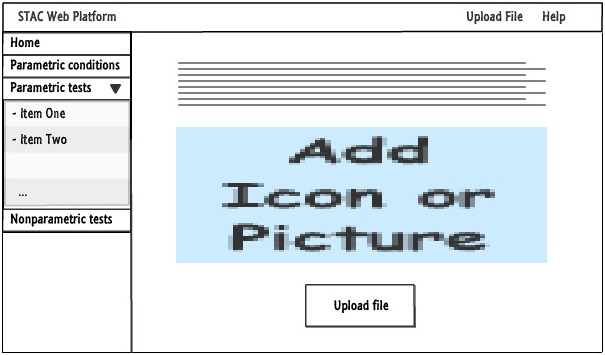
\includegraphics[width=10cm,height=6cm]{figuras/prototipo_home.jpg}
\caption{Prototipo de página principal.}
\label{fig:prot_home}
\end{figure}

\begin{figure}[H]
\centering
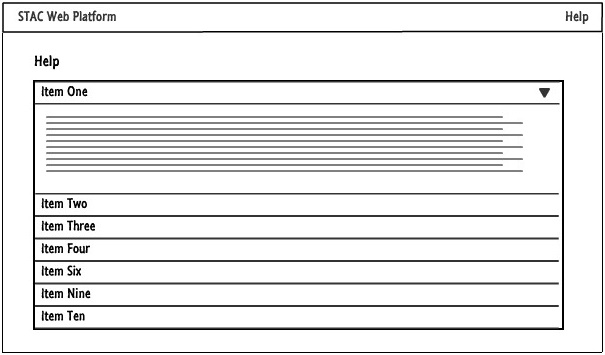
\includegraphics[width=10cm,height=6cm]{figuras/prototipo_help.jpg}
\caption{Prototipo página de ayuda.}
\label{fig:prot_help}
\end{figure}

\begin{figure}[H]
\centering
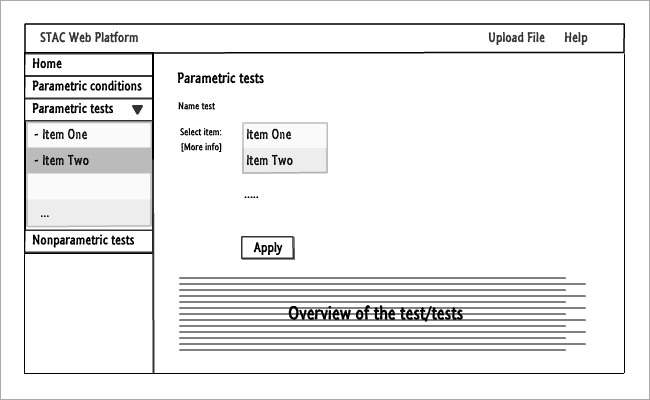
\includegraphics[width=10cm,height=6cm]{figuras/prototipo_test.jpg}
\caption{Prototipo página selección de parámetros/opciones.}
\label{fig:prot_test}
\end{figure}

\begin{figure}[H]
\centering
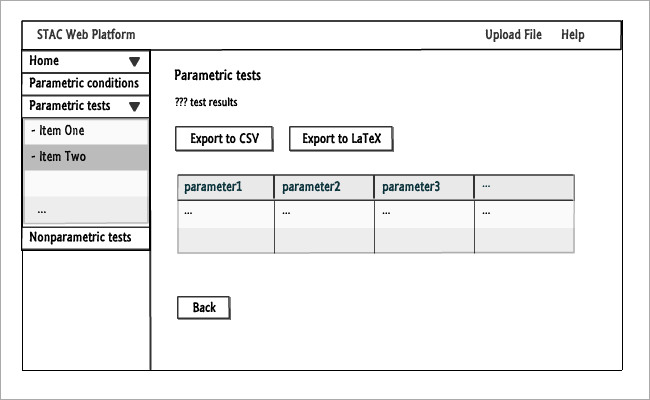
\includegraphics[width=10cm,height=6cm]{figuras/prototipo_results.jpg}
\caption{Prototipo página visualización de resultados.}
\label{fig:prot_results}
\end{figure}

\subsection{Heurísticas de Nielsen}
En la interacción persona-ordenador, se siguen varios pasos para crear sistemas que sean amigables para el usuario. En el paso de evaluación, se pueden realizar pruebas de expertos, en las cuales lo más común es utilizar las heurísticas creadas por Jakob Nielsen para evaluar el diseño de la interfaz de usuario. Los 10 principios de diseño basados en el usuario, que definió Jakob Nielsen en 1990, siguen siendo un referente importante para evaluar la usabilidad de un sitio web. A
continuación se detallan los principios heurísticos de Nielsen, y se comenta en qué medida el sistema cumple con estos principios.

\noindent
\textbf{Visibilidad del estado del sistema}

\textit{El sistema debe siempre mantener a los usuarios informados del estado del sistema, con una realimentación apropiada y en un tiempo razonable.}

El sistema siempre trata de indicar el lugar donde se encuentra el usuario, así como las acciones que puede realizar en el lugar en el que se encuentre. La parte superior de la web trata de indicar estos aspectos mediante títulos / breves descripciones. El menú desplegable de la izquierda también proporciona información del lugar en el que se encuentra el usuario.

\noindent
\textbf{Lenguaje de los usuarios}

\textit{El sistema debe hablar el lenguaje de los usuarios, con las palabras, las frases y los conceptos familiares, en lugar de que los términos estén orientados al sistema. Utilizar convenciones del mundo real, haciendo que la información aparezca en un orden natural y lógico.}

Si bien esta plataforma web está dirigida a gente que posee ciertos conocimientos en algoritmos de aprendizaje automático, puede que estos usuarios no tengan conocimientos suficientes acerca de la validación de resultados mediante la aplicación de test estadísticos y el contraste de hipótesis en general. Por este motivo, el sistema pretende de la forma más amigable posible explicar para qué sirve cada test, los conceptos básicos relacionados con el contraste de hipótesis y cómo interpretar los resultados obtenidos.

\noindent
\textbf{Control y libertad para el usuario}

\textit{Los usuarios eligen a veces funciones del sistema por error y necesitan a menudo una salida de emergencia claramente marcada, esto es, salir del estado indeseado sin tener que pasar por un diálogo extendido. Es importante disponer de deshacer y rehacer.}

El sistema proporciona un botón para volver atrás después de la aplicación de los test dando la posibilidad de cambiar los parámetros u opciones de los mismos. Además, la barra superior contiene en el título de la plataforma un enlace directo a la página principal (de forma similar a la mayoría de las páginas web actuales). En cuanto a la subida de ficheros, el panel emergente que se despliega puede ser cerrado mediante un botón del propio panel o haciendo clic en cualquier lugar de la pantalla, lo cual favorece la cancelación de la acción. Por otra parte, el menú desplegable a la izquierda tiene enlaces directos a los diferentes aspectos de la plataforma (incluido también a la página principal).

\noindent
\textbf{Consistencia y estándares}

\textit{Los usuarios no deben tener que preguntarse si las diversas palabras, situaciones, o acciones significan la misma cosa. En general siga las normas y convenciones de la plataforma sobre la que se está implementando el sistema.}

Se mantiene un lenguaje homogéneo intentando no ser repetitivo y procurando no expresar en distintos lugares las mismas cosas de forma diferente. Además, la simplicidad del sistema favorece que no se produzcan este tipo de dudas en los usuarios.

\noindent
\textbf{Ayuda a los usuarios para reconocimiento, diagnóstico y recuperación de errores}

\textit{Los mensajes de error se deben expresar en un lenguaje claro (no haya códigos extraños), se debe indicar exactamente el problema, y deben ser constructivos.}

En caso de error, se muestra un mensaje indicado claramente el motivo, de forma que el usuario pueda volver a realizar la acción corrigiendo el problema. Estos mensajes no contienen ningún tipo de código e intentan indicar cómo solucionar el problema. Por ejemplo, si se aplican test paramétricos sin haber realizado los test para determinar si los datos cumplen con las condiciones paramétricas, el sistema muestra un mensaje indicando que los resultados devueltos puede que no sean fiables e indica los test que se deberían aplicar.

\noindent
\textbf{Prevención de errores}

\textit{Es importante prevenir la aparición de errores, mejor que generar buenos mensajes de error.}

Se evita que los usuarios tengan que usar campos de texto en los que introducir información, ya que son una de las mayores fuentes de errores. En su lugar se utilizan botones y menús desplegables. El sistema también cuenta con enlaces a la ayuda como una forma de evitar que el usuario cometa errores.

\noindent
\textbf{Reconocimiento antes que cancelación}

\textit{El usuario no debería tener que recordar la información de una parte de diálogo para otra. Es mejor mantener objetos, acciones, y las opciones visibles que memorizar.}

El usuario siempre tiene la información directamente disponible, sin necesidad de tener que recordarla. Para ellos, en cualquier lugar de la web debajo de la barra superior aparece un título o breve descripción que indica claramente en qué lugar se encuentra el usuario. Además, en la pantalla donde se selecciona un test POST-HOC después de la selección del test de ranking principal se muestra el test de ranking previamente seleccionado.

\noindent
\textbf{Flexibilidad y eficiencia de uso}

\textit{Las instrucciones para el uso del sistema deben ser visibles o fácilmente accesibles siempre que se necesiten. Los aceleradores no vistos por el usuario principiante, mejoran la interacción para el usuario experto de tal manera que el sistema puede servir para usuarios inexpertos y experimentados. Es importante que el sistema permita personalizar acciones frecuentes.}

La plataforma dispone de servicios web basados en REST que escuchan permanentemente en \texttt{/api/}, permitiendo a un usuario experto (p. ej. un desarrollador conocedor del sistema) poder introducir en la propia URL los parámetros de los test y el servicio al que desea acceder sin necesidad de interactuar con la interfaz web tal y como lo haría un usuario normal (p. ej. \texttt{http://localhost/api/ttest/id\_fichero/0.05}). Los resultados en este caso se mostrarían en formato JSON, lo cual no resulta visualmente atractivo para un usuario corriente.

\noindent
\textbf{Estética de diálogos y diseño minimalista}

\textit{No deben contener información que sea inaplicable o se necesite raramente. Cada unidad adicional de información en un diálogo compite con las unidades relevantes de información y disminuye su visibilidad relativa.}

La web proporciona descripciones generales o resúmenes de cada test, que pueden resultar muy útiles al usuario no experimentado que necesite tener una idea clara del uso de cada test. Con el objetivo de que esta información extra no interfiera con la selección de opciones y aplicación de los test, se posiciona en la parte inferior de la pantalla (debajo de las opciones).

\noindent
\textbf{Ayuda general y documentación}

\textit{Aunque es mejor si el sistema se puede usar sin documentación, puede ser necesario disponer de ayuda y documentación. Esta ha de ser fácil de buscar, centrada en las tareas del usuario, tener información de las etapas a realizar y que no sea muy extensa.}

La plataforma web cuenta con un botón en la barra superior mediante el cual se puede acceder a la ayuda. En esta ayuda se puede encontrar información acerca del formato del fichero, conceptos básicos, información de test, autoría, etc. Además de este botón, el sistema dispone de diferentes enlaces en lugares clave (opciones de los test, visualización de resultados, etc.) que enlazan con diferentes secciones de la ayuda.

\subsection{Diagramas de secuencia}
Como se ha comentado en el capítulo \ref{arquitecturayh}, los diagramas de secuencia indican los componentes que forman parte del sistema y las llamadas que se hacen en cada uno de ellos para realizar una tarea determinada. Los mensajes o llamadas intercambiados están ordenados temporalmente (en secuencia). A continuación se explicarán los diagramas de secuencia para las funcionalidades más relevantes del sistema.

% Diagramas de secuencia.
\begin{enumerate}

\begin{figure}[H]
\centering
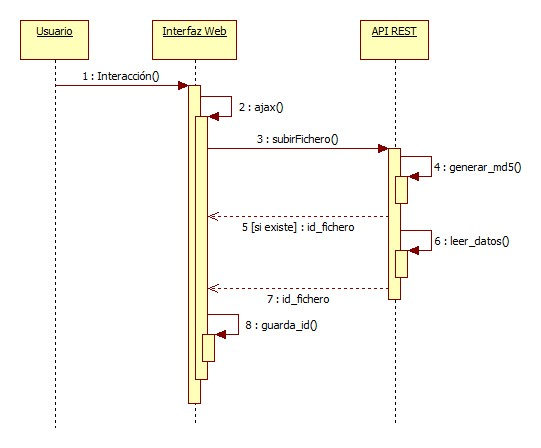
\includegraphics[scale=0.5]{figuras/sec_subir_fichero.jpg}
\caption{Diagrama de secuencia de la subida de ficheros.}
\label{fig:sec_subir_fichero}
\end{figure}

\item En la figura \ref{fig:sec_subir_fichero} podemos ver el diagrama de secuencia para la subida de ficheros de datos. Los objetos Interfaz Web y API REST representan a aquellos ficheros que componen la interfaz web (documentos HTML, CSS, JavaScript etc.) y aquellos que constituyen los servicios web REST (fichero de los servicios y la librería Bottle) respectivamente. Así mismo, la clase \textit{LimitedSizeDict} representa la clase utilizada para limitar el número de ficheros subidos (diccionario con límite de elementos). En primer lugar, el usuario interacciona con la interfaz, donde pulsa el botón para subir un fichero. En la ventana emergente, selecciona el fichero y pulsa el botón \textit{Subir fichero}. Esto desencadena una llamada AJAX al servicio de subida de ficheros del API REST: \textit{subir\_fichero()}. Esta llamada AJAX añade varios parámetros, como el contenido del fichero, el tipo de llamada a realizar (en este caso POST, pues se envían datos al servidor) o el tipo de datos que se esperan de vuelta (que para este proyecto siempre será JSON, como se indicó en el capítulo \ref{arquitecturayh}). Una vez en el servicio web, se obtiene el contenido del fichero especificado en la llamada AJAX con \textit{obtener\_fichero()}. Sobre este contenido, se aplica un algoritmo de reducción criptográfico denominado MD5: \textit{generar\_md5()}, que nos proporciona una clave única para el fichero que lo diferenciará de cualquier otro. Una vez obtenida esta clave, se consulta si existe dicho fichero: \textit{recuperar\_fichero(id)}. Si existe, se devuelve el identificador (en formato JSON) a la aplicación web, que se encargará de guardar en la sesión este identificador para su posterior uso: \textit{guardar\_id(id)}. Si no existe en el diccionario, entonces se invoca a la función \textit{leer\_datos(contenido)}, que determinará si el formato es adecuado y generará un JSON del contenido. Si el formato es adecuado este JSON es almacenado en el diccionario de ficheros con \textit{almacenar(datos)} y finalmente se devolverá el identificador a la interfaz web.


\begin{figure}[H]
\centering
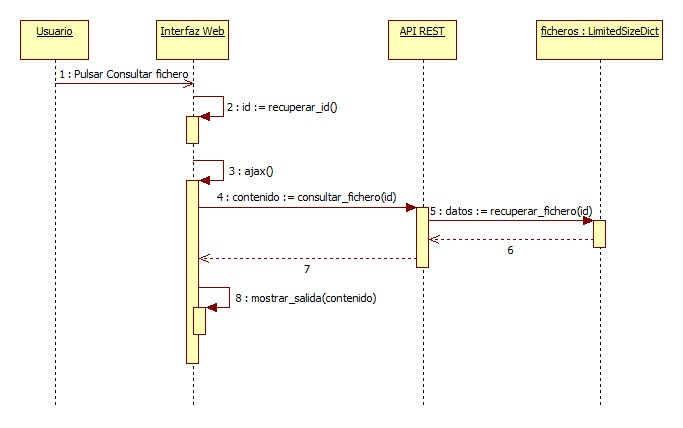
\includegraphics[scale=0.5]{figuras/sec_consultar_fichero.jpg}
\caption{Diagrama de secuencia de la consulta de ficheros.}
\label{fig:sec_consultar_fichero}
\end{figure}

\item En la figura \ref{fig:sec_consultar_fichero} se muestra el diagrama de secuencia para la consulta del fichero. Aquí, en primer lugar el usuario pulsa el botón de \textit{Consultar fichero}. Luego, la interfaz web recupera el identificador de fichero actual almacenado en la sesión: \textit{recuperar\_id()}. A continuación, se realiza la llamada AJAX al servicio web de consulta de ficheros. Esta llamada se diferencia de la anterior en que el método empleado es GET y no POST, pues únicamente se requiere un JSON (contenido del fichero). La llamada al servicio lleva como parámetro obligatorio el identificador del fichero: \textit{consultar\_fichero(id)}. El servicio recupera los datos del fichero: \textit{recuperar\_fichero(id)}, y devuelve el contenido a la interfaz, que se encarga de representar los datos en una tabla y mostrarlos mediante \textit{mostrar\_salida(contenido)}.

\begin{figure}[H]
\centering
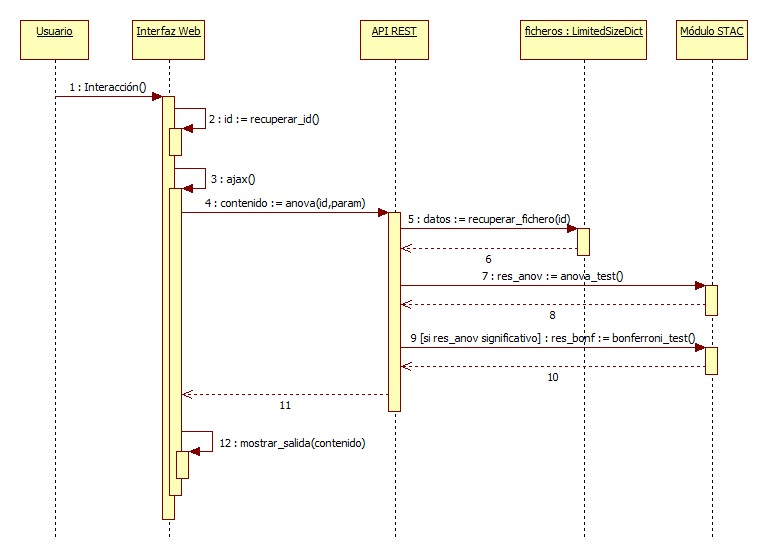
\includegraphics[scale=0.5]{figuras/sec_anova.jpg}
\caption{Diagrama de secuencia del test de ANOVA.}
\label{fig:sec_anova}
\end{figure}

\item La realización del test paramétrico ANOVA se muestra en el diagrama \ref{fig:sec_anova}. En este caso, el usuario accede a la sección de ANOVA en el apartado de test paramétricos, selecciona las opciones disponibles y aplica el test. La llamada al servicio, además del identificador del fichero, en este caso podría llevar más parámetros, como se muestra en la llamada a la función del servicio: \textit{anova(id,param)}. Estos parámetros se muestran en la sección \ref{dis_api}. En este caso, se tiene como parámetro opcional únicamente el nivel de significancia ``alpha". Una vez dentro del servicio web para ANOVA se accede al contenido del fichero de datos almacenado en el diccionario: \textit{recuperar\_fichero(id)} y se procede a realizar la llamada al test estadístico del módulo STAC: \textit{anova\_test()}. Los argumentos para los test se muestran en la sección \ref{dis_py}. Una vez obtenidos los datos (siempre en formato JSON), si el resultado de la prueba de ANOVA es estadísticamente significativa, se procede a aplicar el test POST-HOC de Bonferroni. Una vez aplicados los test se devuelve un JSON desde la API REST a la interfaz web con los resultados. Aquí nuevamente mediante \textit{mostrar\_salida(contenido)} se muestran los resultados del test de ANOVA en una tabla y, si hay resultados para el test POST-HOC de Bonferroni, se genera otra tabla para estos resultados.

\begin{figure}[H]
\centering
\begin{adjustwidth}{-5em}{-5em}
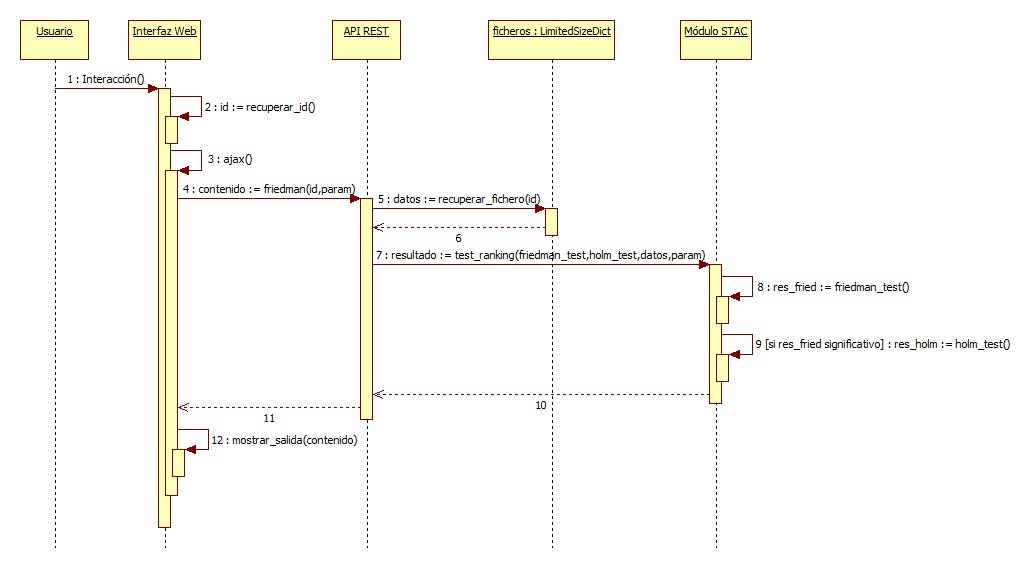
\includegraphics[scale=0.5]{figuras/sec_ranking.jpg}
\caption{Diagrama de secuencia de los test no paramétricos de ranking.}
\label{fig:sec_ranking}
\end{adjustwidth}
\end{figure}

\item En el diagrama de la figura \ref*{fig:sec_ranking} podemos ver el diagrama de secuencia para la realización de test de ranking. En este caso, la interacción del usuario con la interfaz implica posicionarse en la sección de test de ranking dentro de los test no paramétricos y seleccionar las opciones de aplicación de un test determinado. En este diagrama se muestra el ejemplo para la realización del test de Friedman junto con el test POST-HOC de Holm. Sin embargo, esto sería aplicable para todos los test de ranking. Como se ha dicho anteriormente, tanto los parámetros de los servicios como los parámetros de las funciones de los test se muestran en las secciones \ref{dis_api} y \ref{dis_py} respectivamente. Este tipo de test se caracterizan por la invocación de la función \textit{test\_ranking(friedman\_test,holm\_test,datos,param)}, que permite separar los test POST-HOC de los test de ranking, evitando tener que pasar como argumento al test POST-HOC el test de ranking realizado previamente. Dentro de esta función, se realiza el test de Friedman: \textit{friedman\_test()} y si su resultado es estadísticamente significativo, se realiza el test POST-HOC de Holm: \textit{holm\_test()}, de forma similar al test de ANOVA.

\item Por último, en la figura \ref{fig:sec_scipy} se muestra el caso de la aplicación de test pertenecientes a la librería SciPy. Por tato, se incluye el objeto Módulo SciPy. El diagrama muestra como caso de ejemplo la aplicación del test de normalidad de Shapiro-Wilk: \textit{shapiro()}. Este test se aplica para cada uno de los algoritmos de aprendizaje automático presentes en el fichero de entrada, con el objetivo de determinar si los datos obtenidos por cada algoritmo siguen una distribución normal. Además, se muestra una segunda interacción del usuario, en la cual éste en la pantalla de visualización de resultados de los test pulsa el botón de \textit{Exportar a formato \LaTeX}. Como se puede apreciar, la interfaz web en este caso invocaría  a la función \textit{exportTableToLaTeX()} para generar el contenido. Ocurriría lo mismo en caso de la exportación de resultados a formato CSV (con la función \textit{exportTableToCSV()}).

\begin{figure}[H]
\centering
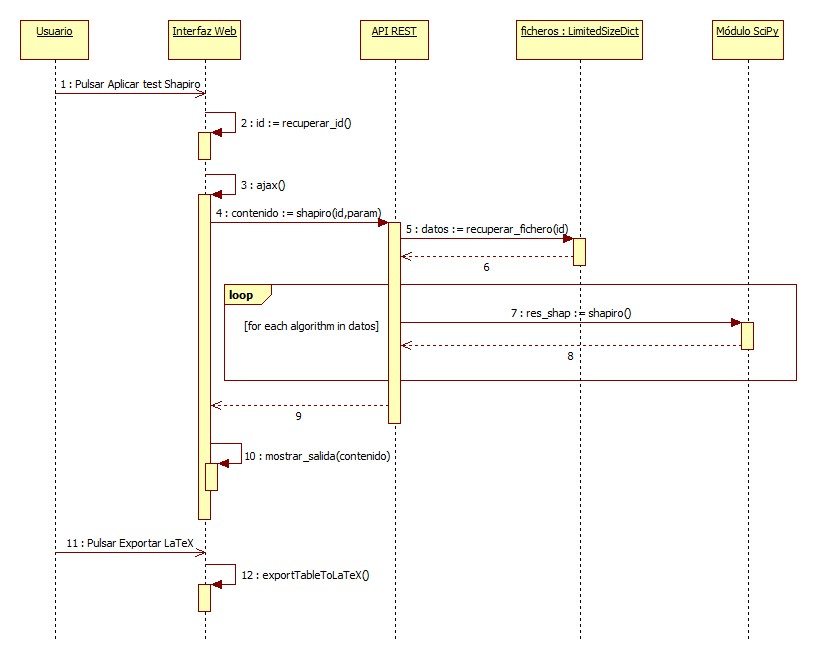
\includegraphics[scale=0.5]{figuras/sec_scipy.jpg}
\caption{Diagrama de secuencia de los test de SciPy.}
\label{fig:sec_scipy}
\end{figure}

\end{enumerate}

\cleardoublepage
\chapter{Validación y pruebas}
Durante y después del proceso de implementación, el programa que se está desarrollando debe ser comprobado para asegurar que satisface su especificación y entrega la funcionalidad esperada por las personas interesadas en el software. La verificación y la validación es el nombre dado a estos procesos de análisis y pruebas. Tienen lugar en cada etapa del proceso del software. Comienza con revisiones de los requerimientos y continúa con revisiones del diseño e inspecciones de código hasta la prueba del producto \cite{sommerville}.

La verificación y la validación no son lo mismo, aunque a menudo se confunden. Boehm \cite{boehm} expresó de forma breve la diferencia entre ellas:

\begin{itemize}
\item \textbf{Verificación:} \textit{¿estamos construyendo el producto correctamente?}
\item \textbf{Validación:} \textit{¿estamos construyendo el producto correcto?}
\end{itemize}

En este capítulo, se detallarán las pruebas de verificación y validación realizadas, para lo cual se llevarán a cabo:
\begin{itemize}
\item \textbf{Pruebas unitarias:} para verificar si los test implementados calculan y devuelven de forma correcta todos los datos necesarios.
\item \textbf{Validación de requisitos (historias de usuario):} para documentar el balance de éxito del proyecto desde el punto de vista del grado de cumplimiento de las historias de usuario.
\end{itemize}

Dada la metodología Scrum vista en la sección \ref{scrum} utilizada en este proyecto, las pruebas cobran mayor importancia a lo largo de todo el ciclo de vida del software (no sólo al final). Esto es debido que el carácter solapado de sus fases ``impone" \space realizar pruebas para verificar que el código se comporta de la manera esperada y en base a las historias de usuario antes de poner fin a cada sprint, ya que es después de la finalización del sprint cuando se establece la reunión de análisis y revisión del incremento generado. En esta reunión, como se comentó en la sección \ref{scrum}, se presenta al cliente (los directores del proyecto) el incremento desarrollado (terminado, probado y operando en un entorno), con el fin de obtener feedback para mejorar e incorporar en sucesivos sprints e ir determinando el balance de éxito en el cumplimiento de las historias de usuario (validación de historias de usuario).

\section{Pruebas unitarias}
Una prueba unitaria es una forma de probar el correcto funcionamiento de un módulo de código. Esto sirve para asegurar que cada uno de los módulos funcione correctamente por separado. Dicho de otra forma, las pruebas unitarias se basan en hacer pruebas en pequeños fragmentos de un programa. Estos fragmentos deben ser unidades estructurales de un programa encargados de una tarea especifica, en programación procedural u orientada a objetos se puede afirmar que estas unidades son los métodos o las funciones que tenemos definidos. En nuestro caso, se han utilizado para comprobar que cada uno de los test estadísticos implementados calcula y devuelve correctamente todos los datos requeridos.

El objetivo de las pruebas unitarias es el aislamiento de partes del código y la demostración de que estas partes no contienen errores. Además, una vez realizados las pruebas unitarias, en caso de que haya que refactorizar algún test estadístico las mismas pruebas pueden servir para probar el nuevo código asegurándonos de que éste sigue siendo válido bajo la nueva implementación.

Durante el ciclo de vida del proyecto se han realizado diferentes fases de pruebas dedicadas especialmente a verificación del correcto funcionamiento de los test. Para aquellos test provenientes de la librería SciPy (de los que hemos hablado en capítulos anteriores), no se han realizado pruebas unitarias, pues ya están verificados por dicha librería.

Para realizar las pruebas unitarias sobre los test implementados se ha utilizado el siguiente marco experimental \cite{no_parametricos}:
\begin{itemize}
\item \textbf{Test no paramétricos de ranking y POST-HOC de comparación simple (con método de control):} 24 problemas o conjuntos de datos de UCI \cite{uci} (repositorio de aprendizaje automático) y KEEL \cite{keel} (repositorio de conjuntos de datos), sobre los que se aplicaron 4 algoritmos clásicos (de búsqueda dispersa, optimización de nube de partículas, etc.): PDFC, NNEP, IS-CHC + 1NN, FH-GBML.
\item \textbf{POST-HOC de comparación múltiple:} Ranking obtenido por el test de Friedman aplicado en 30 conjuntos de datos de UCI y KEEL sobre los que se aplicaron 5 algoritmos: C4.5, 1NN, Naïve Bayes, Kernel y CN2.
\end{itemize}

Así mismo, para el caso del test de Wilcoxon, el test de Anova y el test de Bonferroni, se han empleado datos obtenidos de Internet con los que se han podido verificar su correcto funcionamiento. Además, con algunos test se empleó la herramienta STATService 2.0 \cite{statservice} para tener una referencia a mayores de verificación de resultados.

A continuación en el tabla \ref{unitarias} se detallan las pruebas unitarias realizadas, las cuales se han llevado a cabo con el valor 0.05 como de nivel de significancia, ya que es el valor más común:

\begin{center}
\setlength{\belowcaptionskip}{0.5cm}
\begin{longtable}[H]{| p{3cm}| p{7cm} | p{3cm} |}
	\hline
	\rowcolor{Gray}
	\multicolumn{1}{|c|}{\textbf{Test estadístico}} & \multicolumn{1}{|c|}{\textbf{Resultado esperado}} & \multicolumn{1}{|c|}{\textbf{Resultado obtenido}} \\ \hline
	\endfirsthead
	\hline
	\rowcolor{Gray}
	\multicolumn{1}{|c|}{\textbf{Test estadístico}} & \multicolumn{1}{|c|}{\textbf{Resultado esperado}} & \multicolumn{1}{|c|}{\textbf{Resultado obtenido}} \\ \hline
	\endhead
	\caption{Pruebas unitarias realizadas.}
	\label{unitarias}
	\endfoot
	Test de los Rangos Signados de Wilcoxon & Devuelve correctamente el estadístico, el \textit{p-valor} y el resultado, incluyendo también la suma de los rangos positivos y la suma de los rangos negativos. Devuelve error en caso de que los datos tengan resultados de más de 2 algoritmos. & Correcto \\ \hline
	Test de Friedman & Devuelve correctamente el estadístico, el \textit{p-valor} y el resultado, así como los rankings (tanto en maximización como en minimización). & Correcto \\ \hline
	Test de Iman-Davenport & Devuelve correctamente el estadístico (más ajustado que el Friedman) y su \textit{p-valor} correspondiente. & Correcto \\ \hline
	Test de los Rangos Alineados de Friedman & Los mismos datos que Friedman pero para este test. & Correcto \\ \hline
	Test de Quade & Los mismos datos que Friedman pero para este test. & Correcto \\ \hline
	Datos comunes a los test POST-HOC con método de control & Devuelve correctamente los estadísticos (valores Z), los \textit{p-valores} asociados, los nombres de los algoritmos ordenados según los \textit{p-valores}, el método de control y el valor K (número de algoritmos involucrados). & Correcto \\ \hline
	Test de Bonferroni-Dunn & Devuelve correctamente los \textit{p-valores} ajustados, los resultados y el nivel de significación ajustado a partir de los datos obtenidos en la función anterior. & Correcto \\ \hline
	Test de Holm & Devuelve correctamente los \textit{p-valores} ajustados, los resultados y los niveles de significancia ajustados. & Correcto \\ \hline
	Test de Hochberg & Los mismos datos que Holm pero para este test. & Correcto \\ \hline
	Test de Li & Devuelve correctamente los \textit{p-valores} ajustados y los resultados. & Correcto \\ \hline
	Test de Finner & Los mismos datos que Holm pero para este test. & Correcto \\ \hline
	Datos comunes a los test POST-HOC de comparaciones múltiples & Devuelve correctamente los estadísticos (valores Z), los \textit{p-valores} asociados, los nombres de las comparaciones ordenados según los \textit{p-valores} y el número total de comparaciones. & Correcto \\ \hline
	Multitest de Bonferroni-Dunn & Devuelve correctamente los \textit{p-valores} ajustados, los resultados y el nivel de significación ajustado a partir de los datos obtenidos en la función anterior. & Correcto \\ \hline
	Multitest de Holm & Devuelve correctamente los \textit{p-valores} ajustados, los resultados y los niveles de significancia ajustados. & Correcto \\ \hline
	Multitest de Hochberg & Los mismos datos que el multitest de Holm pero para este test. & Correcto \\ \hline
	Multitest de Finner & Los mismos datos que el multitest de Holm pero para este test. & Correcto \\ \hline
	Test de Shaffer & Los mismos datos que el multitest de Holm pero para este test. & Correcto \\ \hline
	Test ANOVA & Devuelve correctamente el resultado, el estadístico, el \textit{p-valor}, las variaciones y los grados de libertad (totales, del tratamiento y del error), los cuadrados medios y los valores medios (algoritmos y media general). & Correcto. \\ \hline
	Test de Bonferroni & Devuelve correctamente el nivel de significancia ajustado, los estadístico (valores t), sus \textit{p-valores} asociados, los resultados y los \textit{p-valores} ajustados. & Correcto \\ \hline
\end{longtable}
\end{center}

\section{Validación de requisitos}

Como se comentó anteriormente, la validación es el proceso de comprobar que el sistema software producido es lo que el usuario realmente quería. Las historias de usuario, descritas en las secciones \ref{hu_desarrollador} y \ref{hu_cliente} correspondientes a las historias de usuario desarrollador y cliente respectivamente, se han ido validando en las diferentes reuniones con los directores del proyecto al final de cada sprint. Para ello, se han tenido en cuenta los criterios de aceptación incluidos en las propias historias de usuario. Estos criterios de aceptación fueron definidos lo antes posible con el fin de ayudar a entender mejor lo que se esperaba del proyecto y poder realizar estimaciones de forma más fácil y precisa. Además, estos criterios también sirvieron de guía para el desarrollo de pruebas unitarias, tal y como hemos visto en la sección anterior, para verificar el correcto funcionamiento de los test estadísticos.

A continuación se muestra la validación de las historias de usuario desarrollador (tabla \ref{validacionhud}):

\begin{center}
\setlength{\belowcaptionskip}{0.5cm}
\begin{longtable}[H]{| p{1cm} | p{4.25cm} | p{1cm} | p{5cm} |}
	\hline
	\rowcolor{Gray}
	\multicolumn{1}{|c|}{\textbf{H. Usuario}} & \multicolumn{1}{|c|}{\textbf{Título}} & \multicolumn{1}{|c|}{\textbf{Resultado}} & \multicolumn{1}{|c|}{\textbf{Comentario}} \\ \hline
	\endfirsthead
	\hline
	\rowcolor{Gray}
	\multicolumn{1}{|c|}{\textbf{H. Usuario}} & \multicolumn{1}{|c|}{\textbf{Título}} & \multicolumn{1}{|c|}{\textbf{Resultado}} & \multicolumn{1}{|c|}{\textbf{Comentario}} \\ \hline
	\endhead
	\caption{Historias de usuario desarrollador.}
	\label{validacionhud}
	\endfoot
	\textbf{HU-1} & Acceder a los test & Hecho & Se proporcionan diferentes URIs. \\ \hline
	\textbf{HU-2} & Gestionar ficheros & Hecho & Se permite la subida y consulta de datos. \\ \hline
	\textbf{HU-3} & Devolver datos JSON & Hecho & Todos los servicios web manejan este formato. \\ \hline
	\textbf{HU-4} & Analizar datos subidos & Hecho & Devolución de error en caso de formato incorrecto. \\ \hline
	\textbf{HU-5} & Limitar ficheros subidos & Hecho & Almacenamiento en diccionario con límite de elementos. \\ \hline
	\textbf{HU-6} & Visualizar información test & Hecho & Módulo STAC y API correctamente comentados.  \\ \hline
\end{longtable}
\end{center}

Ahora pasamos a detallar la validación de las historias de usuario cliente (tabla \ref{validacionhuc}):

\begin{center}
\setlength{\belowcaptionskip}{0.5cm}
\begin{longtable}[H]{| p{2cm} | p{4.25cm} | p{1cm} | p{5cm} |}
	\hline
	\rowcolor{Gray}
	\multicolumn{1}{|c|}{\textbf{H. Usuario}} & \multicolumn{1}{|c|}{\textbf{Título}} & \multicolumn{1}{|c|}{\textbf{Resultado}} & \multicolumn{1}{|c|}{\textbf{Comentario}} \\ \hline
	\endfirsthead
	\hline
	\rowcolor{Gray}
	\multicolumn{1}{|c|}{\textbf{H. Usuario}} & \multicolumn{1}{|c|}{\textbf{Título}} & \multicolumn{1}{|c|}{\textbf{Resultado}} & \multicolumn{1}{|c|}{\textbf{Comentario}} \\ \hline
	\endhead
	\caption{Historias de usuario cliente.}
	\label{validacionhuc}
	\endfoot
	\textbf{HU-7} & Realizar test de ANOVA & Hecho & En caso de ser estadísticamente significativo se proporcionan también los resultados de Bonferroni. \\ \hline
	\textbf{HU-8} & Realizar test t-test & Hecho & La interfaz dispone de una sección donde aplicar el test. \\ \hline
	\textbf{HU-9} & Realizar test de Wilcoxon & Hecho & \\ \hline
	\textbf{HU-10} & Realizar test de Friedman & Hecho & \\ \hline
	\textbf{HU-11} & Realizar test de Iman-Davenport & Hecho & \\ \hline
	\textbf{HU-12} & Realizar test de los Rangos Alineados de Friedman & Hecho & \\ \hline
	\textbf{HU-13} & Realizar test de Quade & Hecho & \\ \hline
	\textbf{HU-14} & Realizar test de Bonferroni-Dunn & Hecho & Tanto el test simple (método de control) como multitest. \\ \hline
	\textbf{HU-15} & Realizar test de Holm & Hecho & \\ \hline
	\textbf{HU-16} & Realizar test de Finner & Hecho & \\ \hline
	\textbf{HU-17} & Realizar test de Hochberg & Hecho & \\ \hline
	\textbf{HU-18} & Realizar test de Li & Hecho & La interfaz dispone de una sección donde aplicar el test. \\ \hline
	\textbf{HU-19} & Realizar test de Shaffer & Hecho & \\ \hline
	\textbf{HU-20} & Realizar test de normalidad & Hecho & Sección en la interfaz para el test de Shapiro-Wilk, D’Agostino–Pearson y Kolmogorov–Smirnov. \\ \hline
	\textbf{HU-21} & Realizar test de Levene & Hecho & La interfaz dispone de una sección donde aplicar el test. \\ \hline
	\textbf{HU-22} & Subir fichero de datos & Hecho & Se dispone de un botón en la barra de navegación superior. \\ \hline
	\textbf{HU-23} & Consultar fichero de datos & Hecho & Se dispone de un botón en la barra de navegación superior y se visualiza automáticamente después de la subida. \\ \hline
	\textbf{HU-24} & Visualizar resultados de los test & Hecho & Los resultados se muestran en forma de tabla. \\ \hline
	\textbf{HU-25} & Exportar los resultados en formato csv & Hecho & Botón en la pantalla de visualización de resultados. \\ \hline
	\textbf{HU-26} & Exportar los resultados en formato \LaTeX & Hecho & Botón en la pantalla de visualización de resultados. \\ \hline
	\textbf{HU-27} & Seleccionar nivel de significancia & Hecho & Combobox con varios niveles. \\ \hline
	\textbf{HU-28} & Seleccionar la función objetivo & Hecho & Combobox en la sección de test de ranking. \\ \hline
	\textbf{HU-29} & Ver ayuda & Hecho & Se dispone de un botón en la barra de navegación superior y de varios enlaces a conceptos concretos. \\ \hline
	\textbf{HU-30} & Recordar el test de ranking & Hecho & Mensaje que indica el test de ranking seleccionado. \\ \hline
	\textbf{HU-31} & Avisar de las condiciones paramétricas & Hecho & Mensaje de alerta si no se comprueban las condiciones paramétricas al aplicar un test paramétrico. \\ \hline
	\textbf{HU-32} & Ver una breve información de los test & Hecho & Se muestra una breve descripción de las hipótesis que se contrastan. \\ \hline
	\textbf{HU-33} & Enlazar con ficheros de ejemplo & Hecho & Enlaces a ficheros de ejemplo. \\ \hline
	\textbf{HU-34} & Aplicación en diferentes pestañas del navegador & Hecho & La plataforma puede operar independientemente en diferentes pestañas con diferentes archivos de datos. \\ \hline
	\textbf{HU-35} & Diseño adaptable & Hecho & Interfaz adaptable a dispositivos de varias resolución. \\ \hline
	\textbf{HU-36} & Idioma & Hecho & Interfaz en inglés. \\ \hline
	\textbf{HU-37} & Flujo de trabajo & Hecho & Imagen en la página principal. \\ \hline
\end{longtable}
\end{center}
\cleardoublepage
\chapter{Valoraciones finales}
Como hemos detallado en la presente memoria, una de las tareas más importantes que se deben llevar a cabo en el aprendizaje automático es la validación de resultados obtenidos por los algoritmos de aprendizaje. El método estándar más aceptado en la actualidad por los analistas de datos es el de la aplicación de test estadísticos sobre los experimentos, que, entre otras utilidades, apoyan la toma de decisiones, como por ejemplo la elección del algoritmo más adecuado.

La aplicación de test estadísticos se engloba en el ámbito de la Inferencia Estadística, que es la parte de la estadística que estudia cómo sacar conclusiones generales (sujetas a un determinado grado de fiabilidad o significancia) para toda la población a partir del estudio de una muestra. En este proyecto de fin de grado, se pretendió desarrollar un sistema con el que poder sacar conclusiones de los resultados obtenidos por diferentes algoritmos sobre distintos conjuntos de datos para determinar, por ejemplo, si los algoritmos podrían tener un rendimiento significativamente diferente y por lo tanto no se podrían considerar iguales.

El objetivo de este Trabajo de Fin de Grado era desarrollar una plataforma web para la validación de experimentación en aprendizaje automático y minería de datos. En concreto, el trabajo descrito en esta memoria se resume en los siguientes puntos:

\begin{itemize}
\item Se extendió una librería de test estadísticos: nonparametric.py, actualmente implementada en Python.
\item Se crearon servicios web basados en REST para facilitar el uso de los test y para poder realizar la subida y consulta de datos (pertenecientes a la aplicación de distintos algoritmos sobre problema o conjuntos de datos).
\item Se desarrolló una interfaz web que hace uso de estos servicios y que muestra los resultados obtenidos.
\end{itemize}

El objetivo era que el analista pudiese introducir en la web los datos obtenidos mediante experimentación y seleccionar el test estadístico que desease utilizar para que, de forma automática, el sistema le mostrase los resultados de la aplicación del test. Así, el sistema permitiría, de un modo fácil y centralizado la validación de resultados mediante el uso de test estadísticos.

\section{Posibles mejoras}

A continuación se indican algunas ampliaciones que se le podrían aplicar a la aplicación desarrollada:

\subsection{Test estadísticos para datos no apareados}
Uno de los puntos a destacar sobre el presente trabajo, es que los test estadísticos desarrollados en este caso sirven para ser aplicados sobre un tipo de datos en particular: datos apareados. Estos datos, son los que tenemos cuando los datos de las muestras pertenecen a los mismos individuos (p. ej. aplicamos dos algoritmos sobre los mismos N conjuntos de datos, obteniendo dos muestras de tamaño N apareadas). Se podría extender la funcionalidad de la plataforma, permitiendo la aplicación de test estadísticos para datos no apareados. Existen actualmente test para este propósito. Por ejemplo, la contraposición para datos no apareados del test de los Rangos Signados de Wilcoxon presente en este proyecto sería el test U de Mann-Whitney.

\subsection{Datos de entrada}
Otra de las posibles mejoras es poder permitir al usuario la subida de datos no sólo mediante ficheros, sino a través de entrada manual de datos. Además, sería interesante poder permitir al usuario establecer él mismo el formato mediante el cual quiera subir los datos (p. ej. establecer el separador de columnas, el separador de filas, etc.). También se podría disponer de modificación vía web de los datos, tanto si son subidos mediante fichero de entrada o mediante formulario.

\subsection{Otras mejoras}
Se podrían añadir cambios a la interfaz con el fin de hacerla más atractiva al usuario. Por ejemplo: se podría mostrar una barra de progreso en la subida de datos. También se podría dar la posibilidad de mostrar los resultados con un determinado número de decimales (establecido por el usuario).
\cleardoublepage

% Aquí empiezan los apéndices.
\appendix
\cleardoublepage
\chapter{Manual técnico}
En este apéndice se muestra el manual de despliegue de la aplicación, pensado para que los usuarios puedan configurar y poner en funcionamiento la plataforma en sus equipos \footnote{Recordemos que, en cualquier caso, la plataforma web está actualmente disponible en la URL: \\ \textit{\url{http://tec.citius.usc.es/stac/}}}. Para ello, se tomará como base el Sistema Operativo Ubuntu 14.04, junto con Apache 2.4. Las razones de realizar el despliegue con Apache y no con el propio servidor de Bottle se detallan en la sección \ref{tecnologias}. En la figura \ref{fig:directorio_proy}, podemos ver los sub directorios que forman parte del directorio del proyecto:

\begin{figure}[H]
\centering

\includegraphics[scale=0.5]{figuras/directorio_proy.png}
\caption{Directorio del proyecto STAC.}
\label{fig:directorio_proy}
\end{figure}

\begin{itemize}
\item \textbf{api:} API REST (servicios web, archivo de la librería de Bottle y archivo app.wgi).
\item \textbf{documentación:} archivos de la memoria y documentación de los test estadísticos con Sphinx.
\item \textbf{stac:} módulo Python de los test estadísticos.
\item \textbf{web:} archivos web (Framework Bootstrap, CSS, JavaScript, imágenes, ficheros de datos de entrada de ejemplo, etc.).
\end{itemize}

\section{Despliegue de la aplicación en Apache}

\begin{enumerate}
\item Instalar Apache, el módulo WSGI y la librería SciPy:
\newpage
\subitem - \texttt{sudo apt-get install apache2}
\subitem - \texttt{sudo apt-get install libapache2-mod-wsgi}
\subitem - \texttt{sudo apt-get install python-scipy}
\item Crear un enlace simbólico para enlazar el directorio del proyecto al directorio raíz de Apache y cambiar los permisos del directorio raíz \texttt{/var/www}:
\subitem - \texttt{sudo ln -s \$STAC /var/www/stac}
\subitem - \texttt{sudo chmod -R 755 /var/www}
\item El siguiente paso es cambiar la configuración de Apache para que el módulo WSGI cargue la API REST. Para ello se crea el archivo \texttt{/etc/apache2/sites-available/stac.conf} con el siguiente contenido:
\begin{lstlisting}
<VirtualHost *:80>
   ServerName stac
   ServerAlias stac
   
   DocumentRoot /var/www/stac/web
   
   <Directory /var/www/stac/web>
      Order deny,allow
      Allow from all
   </Directory>

   WSGIDaemonProcess stac user=www-data group=www-data processes=1 threads=1
   WSGIScriptAlias /api /var/www/stac/api/app.wsgi
   
   <Directory /var/www/stac/api>
      WSGIProcessGroup stac
      WSGIApplicationGroup \%{GLOBAL}
      Order deny,allow
      Allow from all
   </Directory>

</VirtualHost>
\end{lstlisting}
\item El módulo WSGI buscará el archivo \texttt{/var/www/stac/api/app.wsgi} para cargar la aplicación en el servidor web. El contenido de app.wsgi es el siguiente:
\begin{lstlisting}
import sys, os, bottle
from bottle import route, Bottle

sys.path = ['/var/www/api/'] + sys.path
os.chdir(os.path.dirname(__file__))

import servicios # Importa los servicios REST

application = bottle.default_app() # Carga la aplicacion por defecto con los servicios REST
root = Bottle()
root.mount('/api/', application) # Hacemos que todos los servicios escuchen en /api
\end{lstlisting}
\item Activar el sitio:
\subitem - \texttt{sudo a2ensite stac}
\item Desactivar el sitio por defecto si es necesario:
\subitem - \texttt{sudo a2disite 000-default}
\item Reiniciar servidor:
\subitem - \texttt{sudo service apache2 restart}
\subitem - O también: \texttt{sudo /etc/init.d/apache2 restart}
\end{enumerate}
\cleardoublepage
\chapter{Manual de usuario}

A continuación se explicarán las funcionalidades de la plataforma, apoyándose en capturas de pantalla del sistema.

\section{Página de inicio}

En la figura \ref{fig:man_inicio} se puede ver el aspecto que presenta la página de inicio de la plataforma. En la parte izquierda un menú desplegable permite navegar por los diferentes test que ofrece el sistema: evaluación de condiciones paramétricas, test paramétricos o no paramétricos.

\begin{figure}[H]
\centering
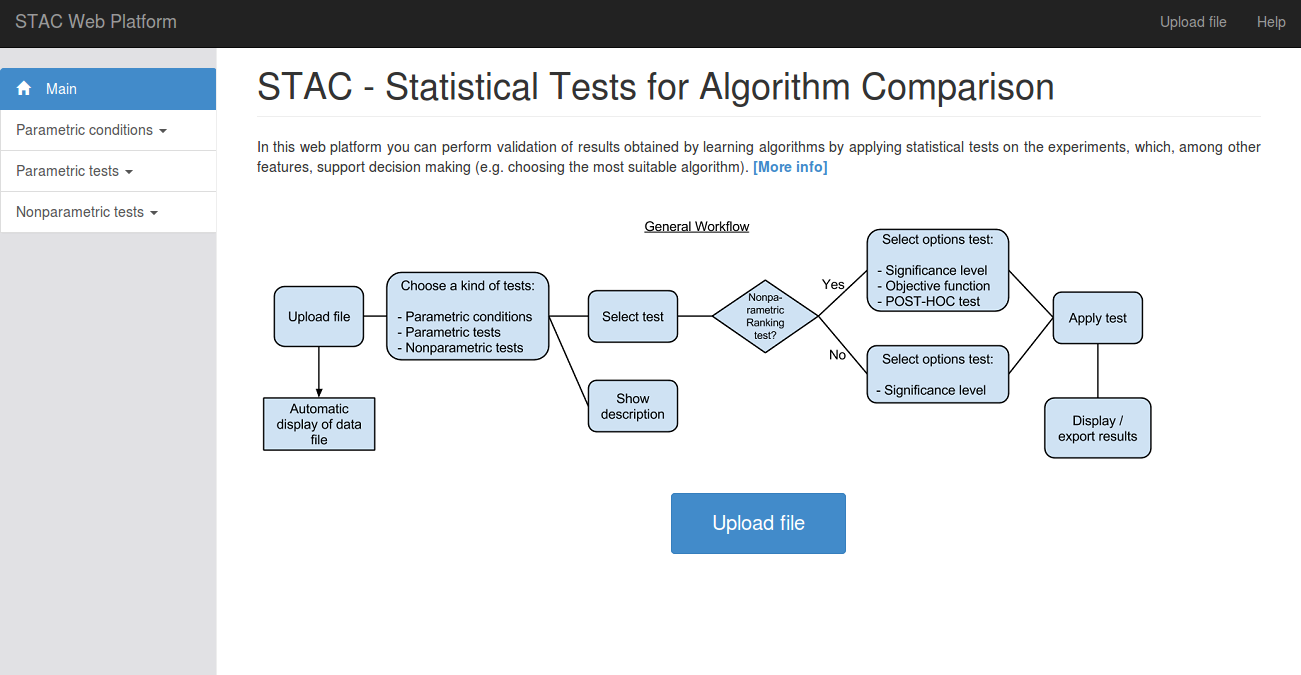
\includegraphics[scale=0.4]{figuras/man_inicio.png}
\caption{Página de inicio de la plataforma.}
\label{fig:man_inicio}
\end{figure}

Así mismo, y con la intención de que los usuarios no familiarizados con la plataforma se puedan hacer una idea de los pasos a seguir en la validación de resultados mediante los test, se presenta una imagen que indica el flujo de trabajo. Debajo de esta imagen, un botón para subir un fichero de datos resalta claramente como primer paso a realizar en la validación. En la figura \ref{fig:man_fichero} se puede ver la ventana emergente que se muestra para la subida de ficheros:

\begin{figure}[H]
\centering
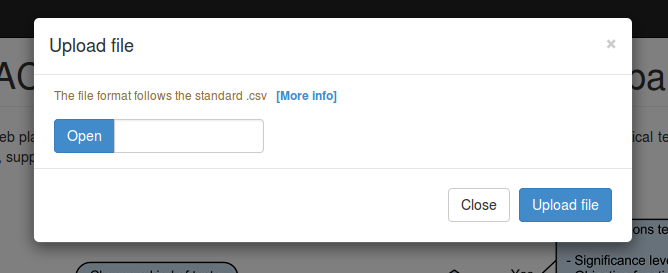
\includegraphics[scale=0.5]{figuras/man_fichero.png}
\caption{Ventana emergente de subida de ficheros.}
\label{fig:man_fichero}
\end{figure}

\begin{figure}[H]
\centering
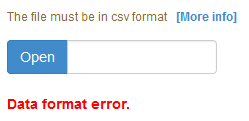
\includegraphics[scale=0.5]{figuras/man_fichero2.png}
\caption{Mensaje de error.}
\label{fig:man_fichero2}
\end{figure}

Para subir el fichero primero se debe hacer clic en ``Open", que abrirá la ventana de búsqueda del fichero. Para subir los datos, se debe hacer clic en ``Upload file". Así mismo, se puede cancelar la acción con ``Close", o haciendo clic en algún otro lugar de la plataforma distinto al de la ventana emergente para la subida de ficheros.

En la figura \ref{fig:man_fichero2}, se muestra un mensaje de error típico cuando los datos no cumplen con el formato especificado. Por otra parte, una barra de navegación superior (común a todas las páginas de la plataforma excepto en la página de ayuda) proporciona un botón de subida de ficheros, consulta de ficheros (después de realizar una subida) y acceso a la ayuda, de forma que desde cualquier página de la plataforma se pueda tanto subir y visualizar ficheros como ir directamente a la ayuda.

\section{Ayuda y consulta de datos}

Las figuras \ref{fig:man_ayuda1} y \ref{fig:man_ayuda2} representan algunas secciones de la ayuda y una sección en particular respectivamente (la del formato del fichero de datos):

\begin{figure}[H]
\centering
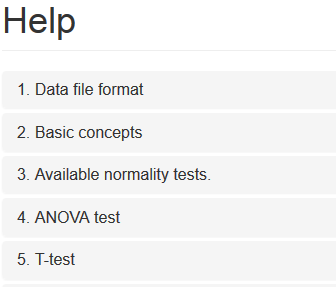
\includegraphics[scale=0.5]{figuras/man_ayuda1.png}
\caption{Listado secciones ayuda.}
\label{fig:man_ayuda1}
\end{figure}

A esta ayuda se accede, como se ha comentado anteriormente, a través de la barra de navegación superior. Sin embargo, la aplicación cuenta también con enlaces que permiten acceder directamente a secciones particulares de la ayuda. Como se puede apreciar en la ventana emergente de subida de ficheros (Fig. \ref{fig:man_fichero}), el enlace \texttt{[more info]} permite realizar esta acción, que nos llevaría a la página representada en la figura \ref{fig:man_ayuda2}. En toda la aplicación existen enlaces de este tipo (la mayoría de los cuales están dedicados a los test de la plataforma.)

\begin{figure}[H]
\centering
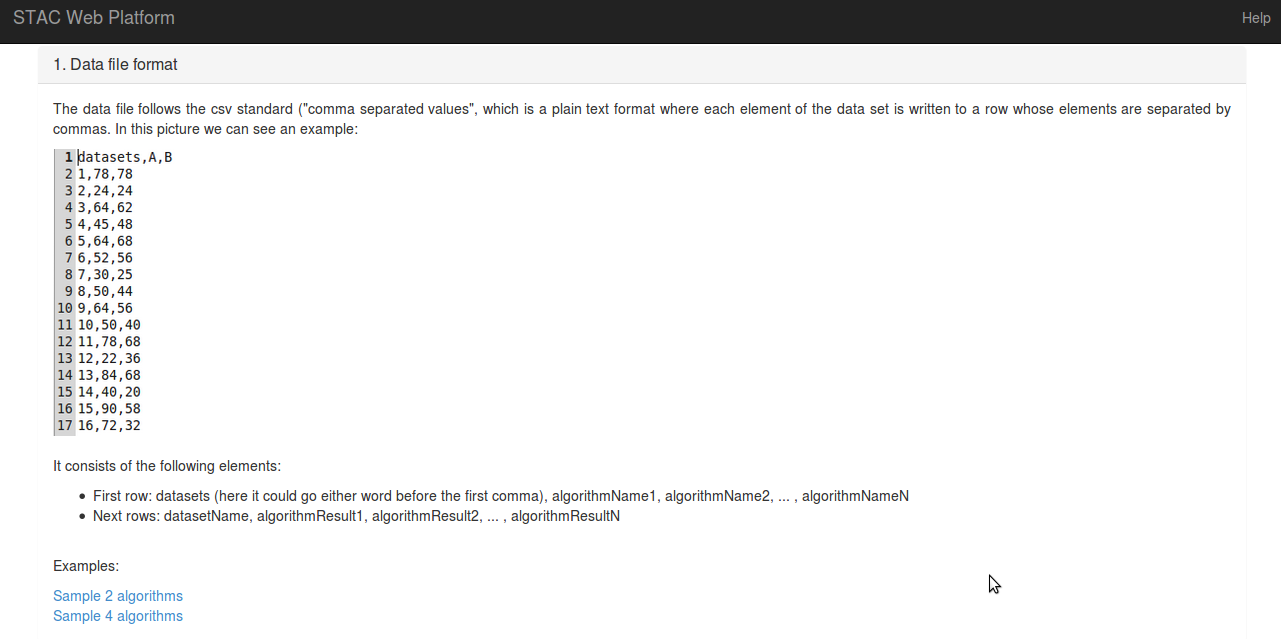
\includegraphics[scale=0.4]{figuras/man_ayuda2.png}
\caption{Sección del formato del fichero de datos.}
\label{fig:man_ayuda2}
\end{figure}

Por otra parte, en la figura \ref{fig:man_consulta} se muestra el aspecto de la pantalla de visualización del contenido del fichero. En esta pantalla, se resalta con un tono azul (similar al usado en los menús y botones del sistema) la línea de datos en la que está posicionado el ratón, con el fin de ayudar en la lectura.

\begin{figure}[H]
\centering
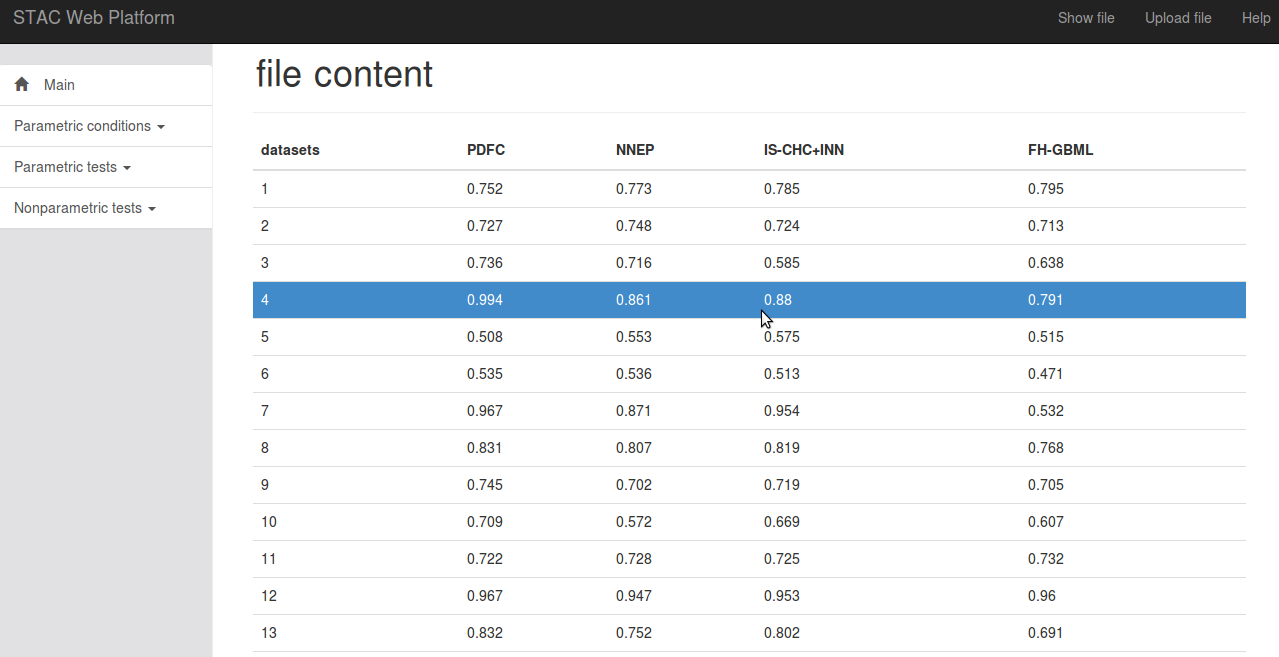
\includegraphics[scale=0.4]{figuras/man_consulta.png}
\caption{Pantalla de visualización del fichero de datos.}
\label{fig:man_consulta}
\end{figure}

\section{Selección de parámetros / opciones de test}

En cada sección en el menú desplegable de la izquierda (condiciones paramétricas, test paramétricos o no paramétricos) aparece como primera opción una descripción general de los test. Por ejemplo en la figura \ref{fig:man_descripcion} se puede ver la descripción de las condiciones paramétricas:

\begin{figure}[H]
\centering
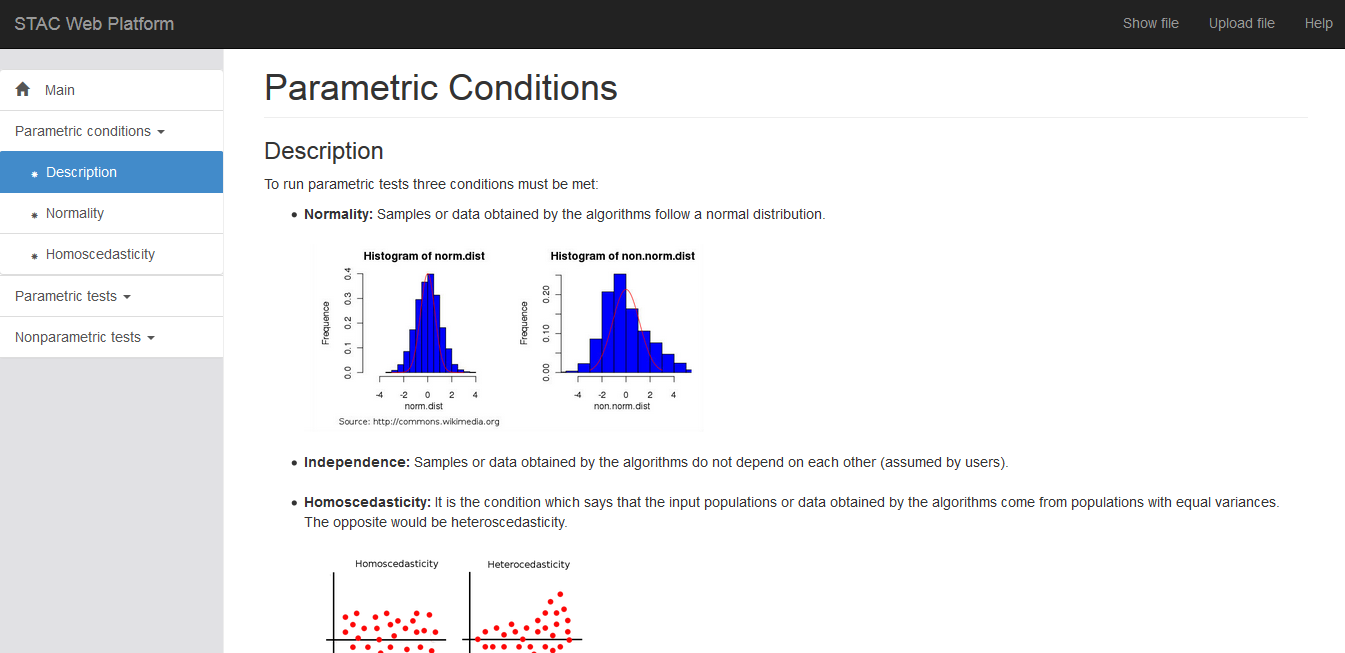
\includegraphics[scale=0.4]{figuras/man_descripcion.png}
\caption{Descripción de test de condiciones paramétricas.}
\label{fig:man_descripcion}
\end{figure}

Cuando se selecciona un tipo de test determinado, la pantalla que se muestra permite la selección de un test en caso de que haya varios disponibles y sus opciones. Por ejemplo en la figura \ref{fig:man_opciones} podemos ver las opciones disponibles para el caso de la sección de test de normalidad. En la parte superior disponemos de las distintas opciones. En la parte inferior se dispone de las descripciones, para que no interfieran en el proceso de aplicación de los test:

\begin{figure}[H]
\centering
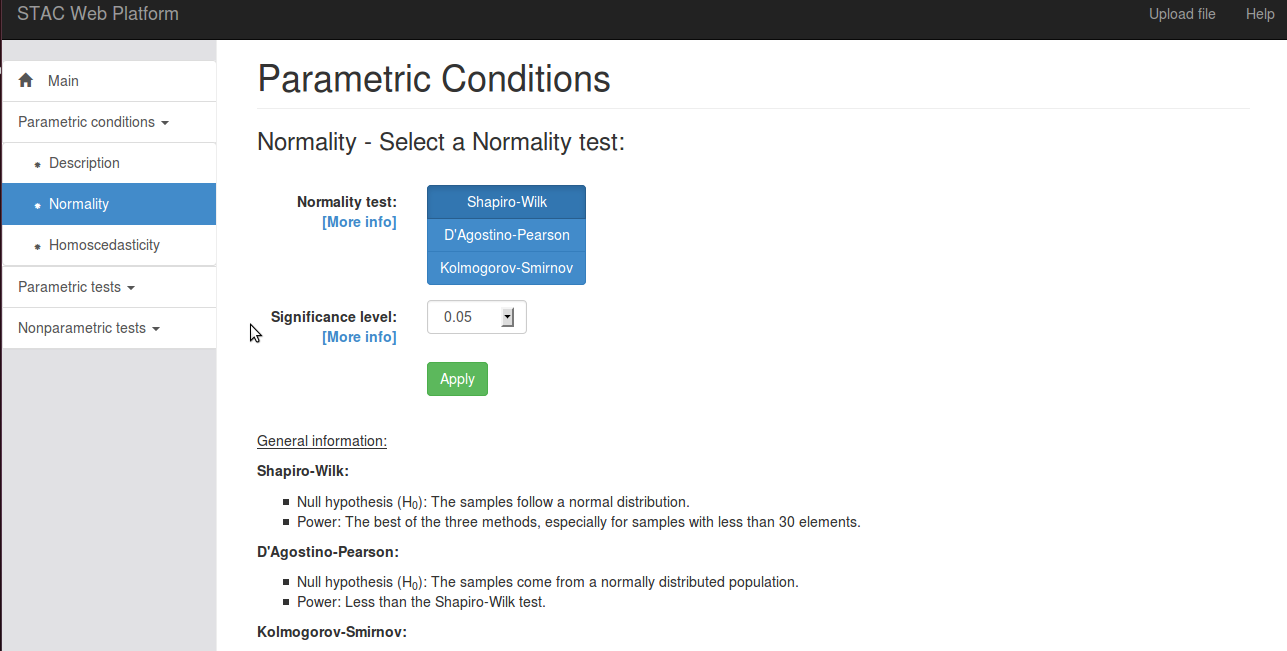
\includegraphics[scale=0.4]{figuras/man_opciones.png}
\caption{Selección de opciones.}
\label{fig:man_opciones}
\end{figure}

Como se puede ver, para cada opción existe un enlace directo a la sección de la ayuda que lo explica. Hay que destacar que no se puede aplicar ningún test en caso de que no exista un fichero de datos subido en la plataforma. En la figura \ref{fig:man_nofichero} se muestra el mensaje de error que se genera al querer aplicar un test sin datos. Por otra parte, ciertos test, como el T-Test o el test de Wilcoxon requieren únicamente ficheros de datos en los que sólo haya datos para dos algoritmos. Si se intenta aplicar estos test sobre ficheros con datos para más de dos algoritmos se genera un error como el que se muestra en la figura \ref{fig:man_errorapli}:

\begin{figure}[H]
\centering
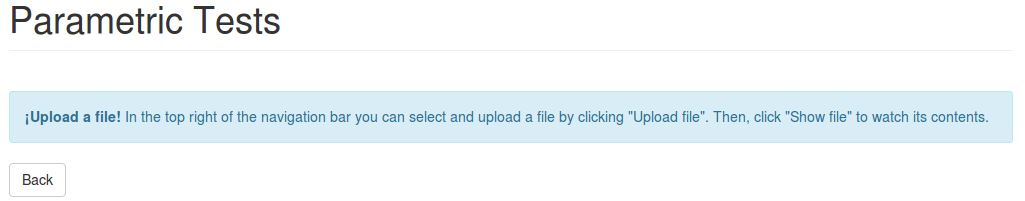
\includegraphics[scale=0.5]{figuras/man_nofichero.png}
\caption{Error cuando no existe ningún fichero.}
\label{fig:man_nofichero}
\end{figure}

\begin{figure}[H]
\centering
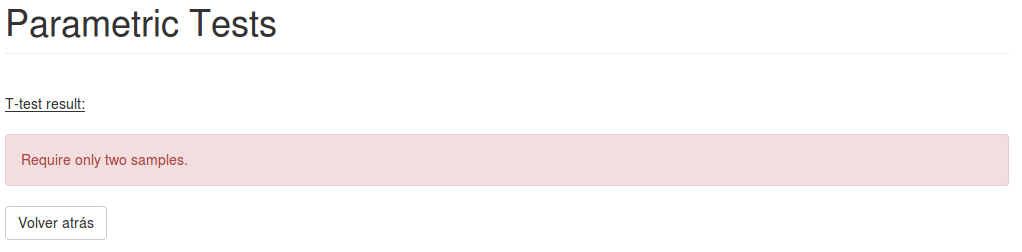
\includegraphics[scale=0.5]{figuras/man_errorapli.png}
\caption{Error cuando el número de algoritmos es mayor a 2.}
\label{fig:man_errorapli}
\end{figure}

También se muestran mensajes de aviso en caso de que se aplique un test paramétrico sin haber comprobado previamente si los datos cumplen con las condiciones paramétricas.

\section{Visualización de resultados}

Después de aplicar algún test, se muestra la pantalla con los resultados obtenidos representados en forma de tabla. En la figura \ref{fig:man_results} podemos ver la pantalla que se genera para mostrar los resultados. En este ejemplo en concreto se muestran los resultados obtenidos después de la aplicación de un test de ranking y un test POST-HOC, para los cuales se generan dos tablas:

\begin{figure}[H]
\centering
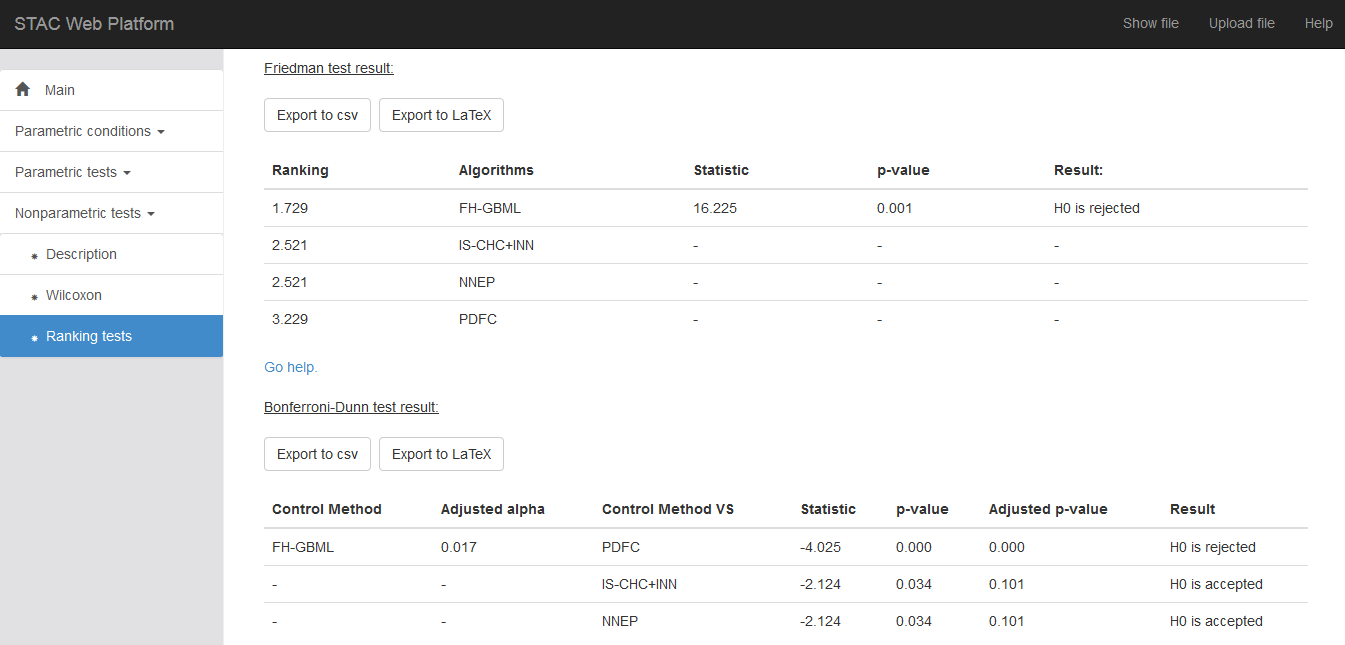
\includegraphics[scale=0.4]{figuras/man_results.png}
\caption{Página de visualización de resultados.}
\label{fig:man_results}
\end{figure}

Así mismo, en cada tabla se muestra la opción de exportar los resultados (tanto a formato \LaTeX \space como a formato CSV). Si se pulsa en uno de estos botones se abre una ventana de diálogo similar a la mostrada en la figura \ref{fig:man_dialog} para poder guardar el fichero generado:

\begin{figure}[H]
\centering
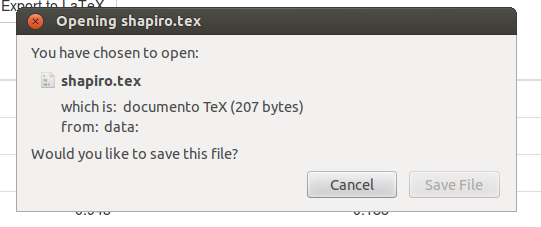
\includegraphics[scale=0.6]{figuras/man_dialog.png}
\caption{Ventana de diálogo exportación resultados.}
\label{fig:man_dialog}
\end{figure}

En las figuras \ref{fig:man_latex} y \ref{fig:man_csv} se muestra cómo sería el contenido de los resultados exportados (en \LaTeX \space y CSV respectivamente) para otro caso de ejemplo (resultados generados en la aplicación del test de normalidad de Shapiro-Wilk):

\begin{figure}[H]
\centering
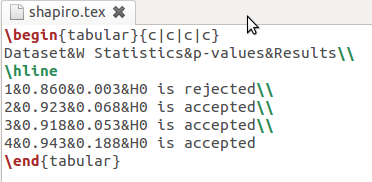
\includegraphics[scale=0.6]{figuras/man_latex.png}
\caption{Formato datos \LaTeX.}
\label{fig:man_latex}
\end{figure}

\begin{figure}[H]
\centering
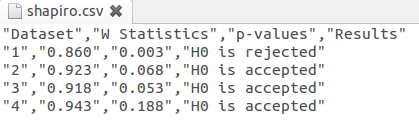
\includegraphics[scale=0.6]{figuras/man_csv.png}
\caption{Formato datos CSV.}
\label{fig:man_csv}
\end{figure}
\cleardoublepage
\markboth{BIBLIOGRAFÍA}{BIBLIOGRAFÍA}

\begin{thebibliography}{99}
% Aprendizaje automático según Mitchell.
\bibitem{mitchell} Tom M. Mitchell, \textit{Machine Learning}, McGraw Hill, 1997.
% Minería de datos.
\bibitem{mineria} Oded Maimon and Lior Rokach, \textit{Data Mining and Knowledge Discovery Handbook}, Springer, New York, 2010.
\end{thebibliography}


\end{document}